%
% Programming in Cryptol
% Galois, Inc.
% Levent Erkok, Dylan McNamee, Joseph Kiniry, and others
%

\documentclass[twoside]{book}
\usepackage{amsfonts}
\usepackage{xspace}
\usepackage{url}
\usepackage{subfigure}
\usepackage{graphicx}
\usepackage{lastpage}
\usepackage{makeidx}
\usepackage[myheadings]{fullpage}
\usepackage{verbatim}
\usepackage{fancyvrb}
\usepackage{booktabs}
\usepackage{amsmath, amsthm, amssymb}
\usepackage{fancyhdr}
\usepackage{xcolor}
\usepackage{pdfpages}
\usepackage[answerdelayed,lastexercise]{utils/exercise}
\usepackage[xetex,bookmarks=true,pagebackref=true,linktocpage=false]{hyperref}
\usepackage[style=list]{utils/glossary}
\usepackage{adjustbox}
\usepackage{xparse}

%% choose output pagesize. Here are two options:
%%  Half of a US Letter sheet, (or A5 paper)
%% intended to be folded in half and bound in a book
% for half-letter:
%\usepackage[paperwidth=5.5in,paperheight=8.5in,inner=62pt,outer=34pt]{geometry}
%\setlength{\textheight}{502pt}

% for full-letter
\usepackage[paperwidth=8.5in,paperheight=11in,inner=62pt,outer=34pt]{geometry}
\setlength{\textheight}{652pt}

\newcommand{\titleline}{Programming in Cryptol}

\hypersetup{%
    pdftitle     = \titleline,
    pdfkeywords  = {Cryptol, Cryptography, Programming},
    pdfauthor    = {Levent Erk\"{o}k and others at Galois},
    pdfpagemode  = UseOutlines
}

\RequirePackage[12tabu,orthodox]{nag}
%
% Programming in Cryptol
% Galois, Inc.
%

% funky symbolic things
\newcommand{\indLamExp}{\index{000lambda@\ensuremath{\lambda}-expression}\xspace}

% operators
\newcommand{\indAppend}{\index{AAAappend@\texttt{\#}, \ (append)}\xspace}
\newcommand{\indIndex}{\index{AAAselect@\texttt{"@}, \ (select)}\xspace}
\newcommand{\indRIndex}{\index{AAAreverseselect@\texttt{"!}, \ (reverse select)}\xspace}
\newcommand{\indIndexs}{\index{AAAselects@\texttt{"@@}, \ (permutation)}\xspace}
\newcommand{\indRIndexs}{\index{AAAreverseselects@\texttt{"!"!}, \ (reverse permutation)}\xspace}
\newcommand{\indShiftLeft}{\index{AAAshiftleft@\texttt{<<}, \ (shift left)}\xspace}
\newcommand{\indShiftRight}{\index{AAAshiftleft@\texttt{>>}, \ (shift right)}\xspace}
\newcommand{\indRotLeft}{\index{AAArotateleft@\texttt{<<<}, \ (rotate left)}\xspace}
\newcommand{\indRotRight}{\index{AAArotateright@\texttt{>>>}, \ (rotate right)}\xspace}
\newcommand{\indOr}{\index{AAAor@\texttt{"|"|}, \ (or)}\xspace}
\newcommand{\indAnd}{\index{AAAandand@\texttt{"\&"\&}, \ (and)}\xspace}
\newcommand{\indXOr}{\index{AAAxor@\texttt{\;\;"\^}, \ (xor)}\xspace}
\newcommand{\indComplement}{\index{AAAcomplement@\texttt{\;\;"\~}, \ (complement)}\xspace}
\newcommand{\indPlus}{\index{AAAplus@\texttt{"+}, \ (add)}\xspace}
\newcommand{\indMinus}{\index{AAAminus@\texttt{"-}, \ (subtract)}\xspace}
\newcommand{\indExponentiate}{\index{AAAexponentiate@\texttt{"\^{}"\^{}}, \ (exponentiate)}\xspace}
\newcommand{\indUnaryMinus}{\index{AAAunaryMinus@\texttt{"-}, \ (unary minus)}\xspace}
\newcommand{\indTimes}{\index{AAAtimes@\texttt{"*}, \ (multiply)}\xspace}
\newcommand{\indDiv}{\index{AAAdiv@\texttt{"/}, \ (divide)}\xspace}
\newcommand{\indMod}{\index{AAAmod@\texttt{"\%}, \ (modulus)}\xspace}
\newcommand{\indEq}{\index{AAAequals@\texttt{"="=}, \ (equal)}\xspace}
\newcommand{\indNeq}{\index{AAequalsnot@\texttt{"!"=}, \ (not-equal)}\xspace}
\newcommand{\indGt}{\index{AAAgreaterthan@\texttt{">}, \ (greater than)}\xspace}
\newcommand{\indGte}{\index{AAAgreaterthanorequal@\texttt{">=}, \ (greater or equal)}\xspace}
\newcommand{\indLt}{\index{AAAlessthan@\texttt{"<}, \ (less than)}\xspace}
\newcommand{\indLte}{\index{AAAlessthanorequal@\texttt{"<=}, \ (less or equal)}\xspace}
\newcommand{\indUnderscore}{\index{AAAunderscore@\texttt{\_}, \ (underscore)}\xspace}

% settings
\newcommand{\indSettingASCII}{\index{settings!\texttt{a},\ (ASCII printing)}\xspace}
\newcommand{\indSettingType}{\index{settings!\texttt{t},\ (printing types)}\xspace}
\newcommand{\indSettingBase}{\index{settings!\texttt{base},\ (output base)}\xspace}
\newcommand{\indSettingEditor}{\index{settings!\texttt{editor},\ (file editor)}\xspace}
\newcommand{\indSettingDefaulting}{\index{settings!\texttt{d},\ (defaulting)}\xspace}
\newcommand{\indSBV}{\index{settings!\texttt{sbv}}\xspace}
\newcommand{\indQCCount}{\index{settings!\texttt{quickCheckCount}}\xspace}

% types
\newcommand{\indTheBitType}{\index{bit}\xspace}
\newcommand{\indTheTupleType}{\index{tuple}\xspace}
\newcommand{\indTheWordType}{\index{word}\xspace}
\newcommand{\indTheIntegerType}{\index{integer}\xspace}
\newcommand{\indTheRationalType}{\index{rational}\xspace}
\newcommand{\indTheFloatType}{\index{float}\xspace}
\newcommand{\indTheSequenceType}{\index{sequence}\xspace}
\newcommand{\indTheRecordType}{\index{record}\xspace}
\newcommand{\indTheStringType}{\index{string}\xspace}
\newcommand{\indTheCharType}{\index{characters}\xspace}

% concepts
\newcommand{\indArbitraryPrecision}{\index{word!arbitrary precision}\xspace}
\newcommand{\indFiniteSeq}{\index{sequence!finite}\xspace}
\newcommand{\indNestedComp}{\index{sequence!nested}\xspace}
\newcommand{\indInfSeq}{\index{sequence!infinite}\xspace}
\newcommand{\indStream}{\index{streams}\xspace}
\newcommand{\indStreamEquation}{\index{stream equations}\xspace}
\newcommand{\indEnum}{\index{sequence!enumerations}\xspace}
\newcommand{\indCartesian}{\index{sequence!cartesian}\xspace}
\newcommand{\indParallel}{\index{sequence!parallel}\xspace}
\newcommand{\indComp}{\index{sequence!comprehensions}\xspace}
\newcommand{\indArithLift}{\index{sequence!arithmetic lifting}\xspace}
\newcommand{\indEndianness}{\index{endianness}\xspace}
\newcommand{\indOverflow}{\index{overflow}\xspace}
\newcommand{\indUnderflow}{\index{underflow}\xspace}
\newcommand{\indModular}{\index{modular arithmetic}\xspace}
\newcommand{\indFloatingPoint}{\index{floating point}\xspace}
\newcommand{\indTypeInference}{\index{type!inference}\xspace}
\newcommand{\indPolymorphism}{\index{type!polymorphism}\xspace}
\newcommand{\indMonomorphism}{\index{type!monomorphism}\xspace}
\newcommand{\indOverloading}{\index{type!overloading}\xspace}
\newcommand{\indUndecidable}{\index{type!undecidable}\xspace}
\newcommand{\indPredicates}{\index{type!predicates}\xspace}
\newcommand{\indTypeClasses}{\index{type!type classes}\xspace}
\newcommand{\indTypeVariables}{\index{type!type variables}\xspace}
\newcommand{\indTypeContext}{\index{type!type context}\xspace}
\newcommand{\indTypeInline}{\index{type!inline argument types}\xspace}
\newcommand{\indTypePositionalArguments}{\index{type!positional arguments}\xspace}
\newcommand{\indAmbiguity}{\index{type!ambiguous}\xspace}
\newcommand{\indSignature}{\index{type!signature}\xspace}
\newcommand{\indTypeAnnotation}{\index{type!annotation}\xspace}
\newcommand{\indFin}{\index{type!\texttt{fin}}\xspace}
\newcommand{\indInf}{\index{type!\texttt{inf}}\xspace}
\newcommand{\indDefaulting}{\index{type!defaulting}\xspace}
\newcommand{\indRecurrence}{\index{recurrences}\xspace}
\newcommand{\indRecursion}{\index{recursion}\xspace}
\newcommand{\indFold}{\index{fold}\xspace}
\newcommand{\indWhileLoop}{\index{while loop}\xspace}
\newcommand{\indPatMatch}{\index{pattern matching}\xspace}
\newcommand{\indProperty}{\index{properties}\xspace}
\newcommand{\indThmFuncCorr}{\index{properties!function correspondence}\xspace}
\newcommand{\indThmCond}{\index{properties!conditional}\xspace}
\newcommand{\indThmPolyvalid}{\index{properties!polymorphic validity}\xspace}
\newcommand{\indQED}{\index{properties!\texttt{Q.E.D.}}\xspace}
\newcommand{\indContradiction}{\index{properties!\texttt{contradiction}}\xspace}
\newcommand{\indProve}{\index{properties!proving}\xspace}
\newcommand{\indProofCompleteness}{\index{properties!completeness}\xspace}
\newcommand{\indCounterExample}{\index{properties!counter-example}\xspace}
\newcommand{\indSat}{\index{satisfiability checking}\xspace}
\newcommand{\indSafe}{\index{safety checking}\xspace}
\newcommand{\indImport}{\index{import directive}\xspace}
\newcommand{\indPrivate}{\index{private qualifier}\xspace}
\newcommand{\indModuleSystem}{\index{module system}\xspace}

% syntax
\newcommand{\indCaseSensitive}{\index{case sensitivity}\xspace}
\newcommand{\indLiterateProgramming}{\index{literate programming}\xspace}
\newcommand{\indComments}{\index{comments}\xspace}
\newcommand{\indFunApp}{\index{function application}\xspace}
\newcommand{\indWhere}{\index{where clause}\xspace}
\newcommand{\indTypSynonym}{\index{type synonym}\xspace}
\newcommand{\indTSWord}{\index{type synonym!Word@\texttt{Word}}\xspace}
\newcommand{\indTSString}{\index{type synonym!String@\texttt{String}}\xspace}
\newcommand{\indTSBool}{\index{type synonym!Bool@\texttt{Bool}}\xspace}

% constants-functions
\newcommand{\indTrue}{\index{True@\texttt{True}}\xspace}
\newcommand{\indFalse}{\index{False@\texttt{False}}\xspace}
\newcommand{\indTake}{\index{take@\texttt{take}}\xspace}
\newcommand{\indTail}{\index{tail@\texttt{tail}}\xspace}
\newcommand{\indDrop}{\index{drop@\texttt{drop}}\xspace}
\newcommand{\indJoin}{\index{join@\texttt{join}}\xspace}
\newcommand{\indSplit}{\index{split@\texttt{split}}\xspace}
\newcommand{\indGroup}{\index{group@\texttt{groupBy}}\xspace}
\newcommand{\indTranspose}{\index{transpose@\texttt{transpose}}\xspace}
\newcommand{\indTupleProj}{\index{project@\texttt{project}}\xspace}
\newcommand{\indLg}{\index{lg2@\texttt{lg2}}\xspace}
\newcommand{\indMin}{\index{min@\texttt{min}}\xspace}
\newcommand{\indMax}{\index{max@\texttt{max}}\xspace}
\newcommand{\indReverse}{\index{reverse@\texttt{reverse}}\xspace}
\newcommand{\indLength}{\index{length@\texttt{length}}\xspace}
\newcommand{\indError}{\index{error@\texttt{error}}\xspace}
\newcommand{\indUndefined}{\index{undefined@\texttt{undefined}}\xspace}
\newcommand{\indAssert}{\index{ASSERT@\texttt{ASSERT}}\xspace}
\newcommand{\indZero}{\index{zero@\texttt{zero}}\xspace}
\newcommand{\indAll}{\index{all@\texttt{all}}\xspace}
\newcommand{\indElem}{\index{elem@\texttt{elem}}\xspace}
\newcommand{\indAny}{\index{any@\texttt{any}}\xspace}
\newcommand{\indPoly}{\index{polynomial}\xspace}
\newcommand{\indDivPoly}{\index{polynomial!division}\xspace}
\newcommand{\indModPoly}{\index{polynomial!modulus}\xspace}
\newcommand{\indMulPoly}{\index{polynomial!multiplication}\xspace}
\newcommand{\indAddPoly}{\index{polynomial!addition}\xspace}
\newcommand{\indSubPoly}{\index{polynomial!subtraction}\xspace}
\newcommand{\indIrredPoly}{\index{polynomial!irreducable}\xspace}

% commands
\newcommand{\indCmdBrowse}{\index{commands!browse@\texttt{:b}\ (browse)}\xspace}
\newcommand{\indCmdLoad}{\index{commands!load@\texttt{:l}\ (load)}\xspace}
\newcommand{\indCmdReload}{\index{commands!reload@\texttt{:r}\ (reload)}\xspace}
\newcommand{\indCmdType}{\index{commands!type@\texttt{:t}\ (type)}\xspace}
\newcommand{\indCmdShell}{\index{commands!shell@\texttt{:"!}\ (shell)}\xspace}
\newcommand{\indCmdEdit}{\index{commands!edit@\texttt{:e}\ (edit)}\xspace}
\newcommand{\indCmdHelp}{\index{commands!help@\texttt{:?}\ (help)}\xspace}
\newcommand{\indCmdQuit}{\index{commands!quit@\texttt{:q}\ (quit)}\xspace}
\newcommand{\indCmdProve}{\index{commands!prove@\texttt{:prove}}\xspace}
\newcommand{\indCmdCheck}{\index{commands!check@\texttt{:check}}\xspace}
\newcommand{\indCmdAutoCheck}{\index{commands!check@\texttt{:check}!automatic}\xspace}
\newcommand{\indCmdSat}{\index{commands!sat@\texttt{:sat}}\xspace}
\newcommand{\indCmdSafe}{\index{commands!safe@\texttt{:safe}}\xspace}
\newcommand{\indCmdLoadModule}{\index{commands!module@\texttt{:m}\ (module load)}\xspace}

% other
\newcommand{\indLineCont}{\index{command line!line continuation}\xspace}
\newcommand{\indCompletion}{\index{command line!completion}\xspace}

% non-Cryptol concepts
\newcommand{\indCipherkey}{\index{cipherkey}\xspace}
\newcommand{\indCiphertext}{\index{ciphertext}\xspace}
\newcommand{\indPlaintext}{\index{plaintext}\xspace}
\newcommand{\indShiftcipher}{\index{shift cipher}\xspace}
\newcommand{\indCaesarscipher}{\index{Caesar's cipher}\xspace}
\newcommand{\indVigenere}{\index{Vigen\`{e}re cipher}\xspace}
\newcommand{\indTranspositioncipher}{\index{transposition cipher}\xspace}
\newcommand{\indScytale}{\index{scytale}\xspace}
\newcommand{\indAtbash}{\index{atbash}\xspace}
\newcommand{\indRailFence}{\index{rail fence cipher}\xspace}
\newcommand{\indKnownPTAttack}{\index{known plaintext attack}\xspace}
\newcommand{\indSubstitutioncipher}{\index{substitution cipher}\xspace}
\newcommand{\indMonoAlphSubst}{\index{substitution cipher!monoalphabetic}\xspace}
\newcommand{\indPolyAlphSubst}{\index{substitution cipher!polyalphabetic}\xspace}
\newcommand{\indPolyGraphSubst}{\index{substitution cipher!polygraphic}\xspace}
\newcommand{\indSubstPeriod}{\index{substitution cipher!period}\xspace}
\newcommand{\indEnigma}{\index{Enigma machine}\xspace}
\newcommand{\indEnigmaPlugboard}{\index{Enigma machine!plugboard}\xspace}
\newcommand{\indEnigmaRotor}{\index{Enigma machine!rotor}\xspace}
\newcommand{\indEnigmaReflector}{\index{Enigma machine!reflector}\xspace}
\newcommand{\indSymKey}{\index{symmetric key}\xspace}
\newcommand{\indAES}{\index{AES}\xspace}
\newcommand{\indGF}{\index{Galois field}\xspace}
\newcommand{\indAESState}{\index{AES!state}\xspace}
\newcommand{\indAESSbox}{\index{AES!SubBytes@\texttt{SubBytes}}\xspace}
\newcommand{\indAESInvSbox}{\index{AES!InvSubBytes@\texttt{InvSubBytes}}\xspace}
\newcommand{\indAESShiftRows}{\index{AES!ShiftRows@\texttt{ShiftRows}}\xspace}
\newcommand{\indAESInvShiftRows}{\index{AES!InvShiftRows@\texttt{InvShiftRows}}\xspace}
\newcommand{\indAESMixColumns}{\index{AES!MixColumns@\texttt{MixColumns}}\xspace}
\newcommand{\indAESInvMixColumns}{\index{AES!InvMixColumns@\texttt{InvMixColumns}}\xspace}

% external tools
\newcommand{\indABC}{\index{ABC}\xspace}
\newcommand{\indYices}{\index{Yices}\xspace}
\newcommand{\indIsabelleHOL}{\index{Isabelle/HOL}\xspace}

%%% Local Variables: 
%%% mode: latex
%%% TeX-master: "../main/Cryptol"
%%% End: 

%%% NB. If you put a citation here, make sure it appears elsewhere in
%%% the document too, otherwise bibtex won't be able to find it!
\newcommand{\glosAES}{\glossary{name=AES, description={The Advanced
Encryption Standard~\cite{aes}}}\xspace}

\newcommand{\glosFibonacci}{\glossary{name=Fibonacci numbers,
description={The sequence $0, 1, 1, 2, 3, 5, \ldots$ After the
elements $0$ and $1$, each consecutive element is the sum of the two
previous numbers~\cite{wiki:fibonacci}}}\xspace}

\newcommand{\glosPlaintext}{\glossary{name=Plaintext, description={A
``readable'' message that we would like to encrypt, the message in the
clear}}\xspace}

\newcommand{\glosCiphertext}{\glossary{name=Ciphertext,
description={The result of encrypting a plaintext message,
``unreadable'' unless the key is known}}\xspace}

\newcommand{\glosCipherkey}{\glossary{name=Cipherkey, description={The
key used in a particular encryption/decryption task}}\xspace}

\newcommand{\glosSAT}{\glossary{name=SAT Solver, description={An
automated tool for solving boolean satisfiability problems. Cryptol
uses SAT/SMT solvers in order to provide its high-assurance
capabilities}}\xspace}

\newcommand{\glosSMT}{\glossary{name=SMT Solver,
description={Satisfiability Modulo Theories: An automated tool for
establishing satisfiability problems with respect to certain
theories. One of the theories of interest to Cryptol is that of
bit-vectors, as it provides a natural medium for translating Cryptol's
bit-precise theorems}}\xspace}

\newcommand{\glosNIST}{\glossary{name=NIST, description={National
Institute of Standards and Technology. The institution in charge of
standardizing cryptoalgorithms (amongst many other things) in
USA.}}\xspace}

\newcommand{\glosGF}{\glossary{name=GF, description={Galois Field. The
notation GF($p^n$) stands for the finite field with $p^n$
elements. For instance, the AES algorithm uses GF($2^8$)
internally~\cite{wiki:galoisfield}}}\xspace}

%%% Local Variables: 
%%% mode: latex
%%% TeX-master: "../main/Cryptol"
%%% End: 

%%%%%%%%%%%%%%%%%%%%%%%%%%%%%%%%%%%%%%%%%%%%%%%%%%%%%%%%%%%%%%%%%%%
%%% The following is copied from book.cls
%%% Beware: if the style changes, change this too
\makeatletter
\renewenvironment{thebibliography}[1]{%
     \chapter*{\bibname
        \@mkboth{\MakeUppercase\bibname}{\MakeUppercase\bibname}}%
\phantomsection
\addcontentsline{toc}{chapter}{Bibliography} 
(Each entry is followed by a list of page numbers on which 
the citation appears. All cited URLs, unless otherwise stated, were last accessed in November 2010.)\\
      \list{\@biblabel{\@arabic\c@enumiv}}%
           {\settowidth\labelwidth{\@biblabel{#1}}%
            \leftmargin\labelwidth
            \advance\leftmargin\labelsep
            \@openbib@code
            \usecounter{enumiv}%
            \let\p@enumiv\@empty
            \renewcommand\theenumiv{\@arabic\c@enumiv}}%
      \sloppy
      \clubpenalty4000
      \@clubpenalty \clubpenalty
      \widowpenalty4000%
      \sfcode`\.\@m}
     {\def\@noitemerr
       {\@latex@warning{Empty `thebibliography' environment}}%
      \endlist}
\makeatother
%%%%%%%%%%%%%%%%%%%%%%%%%%%%%%%%%%%%%%%%%%%%%%%%%%%%%%%%%%%%%%%%%%
%%% index trickery
\makeatletter
\renewenvironment{theindex}{%
                \if@twocolumn
                  \@restonecolfalse
                \else
                  \@restonecoltrue
                \fi
                \columnseprule \z@
                \columnsep 35\p@
                \twocolumn[\@makeschapterhead{\indexname} 
\phantomsection
\addcontentsline{toc}{chapter}{Index}          
%\noindent (Some explanations or yet others totally unrelated but still
%useful might go here or there. no one cares.)\\
		]%
                \@mkboth{\MakeUppercase\indexname}%
                        {\MakeUppercase\indexname}%
                \parskip\z@ \@plus .3\p@\relax
                \let\item\@idxitem}
               {\if@restonecol\onecolumn\else\clearpage\fi}
\makeatother
%%%%%%%%%%%%%%%%%%%%%%%%%%%%%%%%%%%%%%%%%%%%%%%%%%%%%%%%%%%%%%%%%%
%%% toc trickery
\makeatletter
\renewcommand\tableofcontents{%
    \if@twocolumn
      \@restonecoltrue\onecolumn
    \else
      \@restonecolfalse
    \fi
    \chapter*{\contentsname
        \@mkboth{%
           \MakeUppercase\contentsname}{\MakeUppercase\contentsname}}%
\phantomsection                                
\addcontentsline{toc}{chapter}{Contents}   
    \@starttoc{toc}%
    \if@restonecol\twocolumn\fi
}
\makeatother
%%%%%%%%%%%%%%%%%%%%%%%%%%%%%%%%%%%%%%%%%%%%%%%%%%%%%%%%%%%%%%%%%%
%%% lof trickery
\makeatletter
\renewcommand\listoffigures{%
    \if@twocolumn
      \@restonecoltrue\onecolumn
    \else
      \@restonecolfalse
    \fi
    \chapter*{\listfigurename
      \@mkboth{\MakeUppercase\listfigurename}%
              {\MakeUppercase\listfigurename}}%
\phantomsection
\addcontentsline{toc}{chapter}{List of Figures} 
    \@starttoc{lof}%
    \if@restonecol\twocolumn\fi
    }
\makeatother
%%%%%%%%%%%%%%%%%%%%%%%%%%%%%%%%%%%%%%%%%%%%%%%%%%%%%%%%%%%%%%%%%%


% fonts
\usepackage[TS1,T1]{fontenc}
\usepackage{microtype}
\usepackage[osf]{mathpazo}
\usepackage{fontspec}
\usepackage{xunicode}
\usepackage{xltxtra}
\defaultfontfeatures{Mapping=tex-text}
%\setmainfont[]{Times}
%\setsansfont[]{Helvetica}
%\setmonofont[Scale=0.85]{Courier}
\usepackage{sectsty}
\usepackage[disable]{todonotes}
\allsectionsfont{\sffamily}

%% Commands for checking REPL
\DefineVerbatimEnvironment
    {replinVerb}{Verbatim}
    {}
\DefineVerbatimEnvironment
    {reploutVerb}{Verbatim}
    {}
\DefineVerbatimEnvironment
    {replPrompt}{Verbatim}
    {}
\CustomVerbatimCommand{\replin}{Verb}{}
\CustomVerbatimCommand{\replout}{Verb}{}
\NewDocumentCommand{\hidereplin}{r||}{}
\NewDocumentCommand{\hidereplout}{r||}{}
\newcommand{\restartrepl}[0]{}{}

% \newcommand{\todo}[1]{\begin{center}\framebox{\begin{minipage}{0.8\textwidth}{{\bf TODO:} #1}\end{minipage}}\end{center}}
\newcommand{\lamex}{\ensuremath{\lambda}-expression\indLamExp}
\newcommand{\lamexs}{\ensuremath{\lambda}-expressions\indLamExp}
\makeatletter
\def\imod#1{\allowbreak\mkern10mu({\operator@font mod}\,\,#1)}
\makeatother
\newcommand{\advanced}{\begin{center}\framebox{\begin{minipage}{0.95\textwidth}{{\bf Note:} The material in this section
    is aimed for the more advanced reader. It can be skipped on a first reading without loss of continuity.}\end{minipage}}\end{center}}

    \newcommand{\sectionWithAnswers}[2]{%
        \section{#1}\label{#2}%
            \AnswerBoxSectionMark{Section \arabic{chapter}.\arabic{section} #1 (p.~\pageref{#2})}%
            \AnswerBoxExecute{\addcontentsline{toc}{section}{\texorpdfstring{\parbox{2.3em}{\arabic{chapter}.\arabic{section}\ }}{(\arabic{chapter}.\arabic{section})\ }#1}}%
    }

\newcommand{\commentout}[1]{}
\DefineVerbatimEnvironment{code}{Verbatim}{}
\renewcommand{\ExerciseHeaderTitle}{\ExerciseTitle}
\renewcommand{\theExercise}{\thechapter.\arabic{Exercise}}
%\renewcommand{\theExercise}{\thesection--\arabic{Exercise}}
\renewcommand{\ExerciseHeader}{\textbf{\hspace*{-\parindent}\ExerciseName\ \theExercise.\ }}
\renewcommand{\AnswerHeader}{\textbf{\hspace*{-\parindent}\ExerciseName\ \theExercise.\ }}
%\renewcounter{Exercise}[section]
\renewcounter{Exercise}[chapter]
\newcommand{\unparagraph}{\paragraph{$\,\,\,$\hspace*{-\parindent}}}
\newcommand{\exerciseref}[1]{\hyperref[#1]{exercise~\ref*{#1}}}

% various little text sections:
\newtheorem*{hint}{Hint}
\newcommand{\note}[1]{\vspace{5mm}{\setlength{\parindent}{0pt}{\bf Note:~}{#1}}}
\newcommand{\tip}[1]{\vspace{5mm}{\setlength{\parindent}{0pt}{\bf Tip:~}{#1}}}
\newcommand{\lhint}[1]{({\bf Hint}\ #1)}
\newcommand{\ansref}[1]{{\bf (p.~\pageref{#1})}}
%% not needed:?
\setlength{\voffset}{-1cm}

\setlength{\headsep}{2cm}
\setlength{\headheight}{15.2pt}
\renewcommand{\headrulewidth}{0pt} % no line on top
\renewcommand{\footrulewidth}{.5pt} % line on bottom
\renewcommand{\chaptermark}[1]{\markboth{#1}{}}
\renewcommand{\sectionmark}[1]{\markright{#1}{}}
\cfoot{}
\fancyfoot[LE,RO]{\fancyplain{}{\textsf{\thepage}}}
\fancyfoot[LO,RE]{\fancyplain{}{\textsf{\copyright\ 2010--2018, Galois, Inc.}}}
%% \fancyhead[LE]{\fancyplain{}{\textsf{\draftdate}}}
%% \fancyhead[RO]{\fancyplain{}{\textsf{DO NOT DISTRIBUTE!}}}
\fancyhead[RO,LE]{\fancyplain{}{}} %% outer
%\fancyhead[LO,RE]{\fancyplain{}{\textsf{\nouppercase{\rightmark}}}}
\fancyhead[LO,RE]{\fancyplain{}{\textsf{\nouppercase{\rightmark}}}} %% inner
\pagestyle{fancyplain}

\makeglossary
\makeindex

\begin{document}

\title{\Huge{\bf \titleline}}
\author{\\$ $\\$ $\\
    Levent Erk\"{o}k\\
        %\url{levent.erkok@galois.com}
    \\$ $\\
        Galois, Inc.\\
        421 SW 6th Ave., Suite 300\\Portland, OR 97204}
        \date{
            \vspace*{2cm}$ $\\
                
\includegraphics{utils/galois.jpg}
        }

\pagenumbering{roman}

%% for full-size papersize:

\includepdf[offset=0 -28]{cover/CryptolCover.pdf}

%% for A5 / half-letter papersize:
% 
\includepdf[offset=0 -28]{cover/CryptolSmallCover.pdf}


% \maketitle

\index{inference|see{type, inference}}
\index{signature|see{type, signature}}
\index{polymorphism|see{type, polymorphism}}
\index{monomorphism|see{type, monomorphism}}
\index{overloading|see{type, overloading}}
\index{undecidable|see{type, undecidable}}
\index{predicates|see{type, predicates}}
\index{defaulting|see{type, defaulting}}
\index{fin@\texttt{fin}|see{type, fin}}
\index{ambiguous constraints|see{type, ambiguous}}
\index{wildcard|see{\texttt{\_} (underscore)}}
\index{lambda expression|see{\ensuremath{\lambda}-expression}}
\index{pdiv@\texttt{pdiv}|see{polynomial, division}}
\index{pmod@\texttt{pmod}|see{polynomial, modulus}}
\index{pmult@\texttt{pmult}|see{polynomial, multiplication}}
\index{000GF28@GF($2^8$)|see{galois field}}

\setlength{\headsep}{24pt}
% \layout

%%%%%% PREFACE
%\chapter*{Preface}
\addcontentsline{toc}{chapter}{Preface}

Cryptol is a domain-specific language for programming, executing,
testing, and formally reasoning about streams of bits.  It
particularly excels at specifying and reasoning about cryptographic
algorithms.  It has been designed to reduce the gap that currently
exists between the {\it specification} of a cryptographic algorithm
and its executable {\it implementation}.  As a result, a well-written
Cryptol program will look very much like the specification of the
algorithm it implements, and is also executable.  

Our goal in this book is to both teach you the Cryptol language and
provide a reference text for the use of the Cryptol system.  The
Cryptol system provides: (1)~a REPL for experimentation, (2)~a parser
and typechecker for Cryptol programs, (3)~an interpreter for executing
Cryptol programs, (4)~automatically checking the correctness of
Cryptol programs via randomized testing, and (5)~formally verifying
Cryptol programs through the use of an SMT solver.

We demonstrate Cryptol in action via normal programming problems,
traditional cryptographic techniques (such as substitution ciphers),
historical cryptographic mechanisms (such as the Enigma), and modern
algorithms (such as DES, SHA, and AES), focusing on how they are
elegantly modeled using the Cryptol language.  Since our emphasis is
on programming, we introduce some of the techniques that are useful
for the working programmer, including the use of Cryptol's validation
and verification tools that directly support high-assurance
programming.

Our approach is hands on.  We strongly urge the reader to try out the
material using the Cryptol toolset directly.  It would be most
effective to read this document while trying the code and interacting
with Cryptol itself.  For information on how to download and use the
Cryptol toolset, please visit \url{www.cryptol.net}.

Most exercises come with solutions provided at the end. We urge the
readers to refer to solutions as a last resort as they work through
the exercises.

\note{This book covers Cryptol version 2, which is still under
  development.  It is possible that the syntax and semantics for the
  language or commands will change.  You may encounter bugs or
  unexpected behaviors.  Please let us know if you encounter any
  problems, by sending email to {\tt cryptol@galois.com} or by
  visiting our GitHub presence linked from the Cryptol website.}

The authors of this book are Levent {Erk\"{o}k}, Dylan McNamee, Joseph
Kiniry, Iavor Diatchki, and John Launchbury, with contributions from
Magnus Carlsson, Kyle Carter, Trevor Elliott, Adam Foltzer, Brian
Huffman, David Lazar, John Matthews, Eric Mertens, Matt Sottile, Aaron
Tomb, and Adam Wick.

\todo[inline]{Replace manual use of Trac URLs with \texttt{ticket}
  macro everywhere.}

%%% Local Variables: 
%%% mode: latex
%%% TeX-master: "../main/Cryptol"
%%% End: 

\noindent
{\bf IMPORTANT NOTICE}

{\small
  This documentation is furnished for informational use only
  and is subject to change without notice. Galois, Inc.~assumes no
  responsibility or liability for any errors or inaccuracies that may
  appear in this documentation. Of course, we appreciate bug reports
  and clarification suggestions.

  Copyright 2003--2014 Galois, Inc. All rights reserved by Galois,
  Inc.

  The software installed in accordance with this documentation is
  copyrighted and licensed by Galois, Inc.~under separate license
  agreement. This software may only be used pursuant to the terms and
  conditions of such license agreement.}

\noindent
{\bf TRADEMARKS}

{\small 
  Cryptol is a registered trademark of Galois, Inc.~in the United
  States and other countries. UNIX is a registered trademark of The
  Open Group in the U. S.  and other countries. Linux is a registered
  trademark of Linus Torvalds.

  Other company or product names mentioned herein may be trademarks or
  registered trademarks of their respective owners. Trademark
  specifications are subject to change without notice. All terms
  mentioned in this documentation that are known to be trademarks or
  service marks have been appropriately capitalized to the best of our
  knowledge; however, Galois cannot attest to the accuracy of all
  trademark information. Use of a term in this documentation should
  not be regarded as affecting the validity of any trademark or
  service mark.

\vspace{0.5in}
\noindent
Galois, Inc.\\
421 SW Sixth Avenue, Suite 300 \\
Portland, OR 97204
}

%%% Local Variables: 
%%% mode: latex
%%% TeX-master: "../main/Cryptol"
%%% End: 



%%%%%% TOC
\tableofcontents


\includepdf[pages={1}]{cover/Blank.pdf}
\newpage

\setcounter{page}{1}
\pagenumbering{arabic}
%%%%%% Crash Course
\commentout{
\begin{code}
  module CrashCourse where
\end{code}
}

%#####################################################################
\chapter{A Crash Course in Cryptol}
\label{cha:crash-course-cryptol}

Before we can delve into cryptography, we have to get familiar with
Cryptol.  This chapter provides an introduction to Cryptol, just to
get you started. The exposition is not meant to be comprehensive, but
rather as an overview to give you a feel of the most important tools
available.  If a particular topic appears hard to approach, feel free
to skim it over for future reference.

A full language reference is beyond the scope of this document at this
time.
% The language features not covered in this document at this time
% include:
% \begin{itemize}
% \item feature one
% \item feature two
% \end{itemize}
% \todo[inline]{2.1: Add list here of language features not yet
%   covered.}

% TODO The full grammar for Cryptol is included
% in~\autoref{cha:cryptol-grammar}.

%=====================================================================
\section{Basic data types}
\label{sec:basic-data-types}

Cryptol provides five basic data types: bits, sequences, integers,
tuples, and records. Words (i.e., $n$-bit numbers) are a special case
of sequences. Note that, aside from bits and integers, all other
Cryptol types can be nested as deep as you like. That is, we can have
records of sequences containing tuples made up of other records, etc.,
giving us a rich type-system for precisely describing the shapes of
data our programs manipulate.

While Cryptol is statically typed, it uses type inference to supply
unspecified types.  That is, the user does {\em not} have to write the
types of all expressions; they will be automatically inferred by the
type-inference engine.  Of course, in certain contexts the user might
choose to supply a type explicitly.  The notation is simple: we simply
put the expression, followed by {\tt :} and the type. For instance:
\begin{Verbatim}
   12 : [8]
\end{Verbatim}
means the value {\tt 12} has type {\tt [8]}, i.e., it is an 8-bit
word. We shall see other examples of this in the following discussion.

%=====================================================================
\sectionWithAnswers{Bits: Booleans}{sec:bits}

The type {\tt Bit}\indTheBitType represents a single bit of
information. There are precisely two values of this type: {\tt
  True}\indTrue and {\tt False}\indFalse. Bit values play an important
role in Cryptol, as we shall see in detail shortly. In particular, the
test expression in an {\tt if-then-else} statement must have the type
{\tt Bit}.  The logical operators {\tt \&\&}\indAnd (and), {\tt
  ||}\indOr (or), {\tt \Verb|^|}\indXOr (xor), and {\tt
  \Verb|~|}\indComplement (complement) provide the basic operators
that act on bit values.

\begin{Exercise}\label{ex:dataBit}
  Type in the following expressions at the Cryptol prompt, and observe
  the output:
\begin{Verbatim}
  True
  false
  False : Bit
  if True && False then 0x3 else 0x4
  False || True
  (True && False) ^ True
  ~False
  ~(False || True)
\end{Verbatim}
Remember that Cryptol is case sensitive, and hence {\tt false} is
different from {\tt False}.\indCaseSensitive
\end{Exercise}
\begin{Answer}\ansref{ex:dataBit}
Here is the response from Cryptol, in order:
\begin{small}
\begin{Verbatim}
  True
  [error] at <interactive>:1:1--1:6 Value not in scope: false
  False
  0x4
  True
  True
  True
  False
\end{Verbatim}
\end{small}
\end{Answer}

\begin{tip}
  Cryptol provides extensive command line/tab completion; use
  up/down-arrow to see your previous commands, hit tab to complete
  identifier names, etc.
\end{tip}

%=====================================================================
\sectionWithAnswers{Words: Numbers}{sec:words}

A word is simply a numeric value with some number of bits,
corresponding to the usual notion of binary numbers.\indTheWordType To
match our observation of how cryptographers use binary numbers,
Cryptol only supports non-negative ($\geq 0$) word values (i.e., no
floating point or negative numbers).\indFloatingPoint However, words
can be arbitrarily large: There is no predefined maximum number of
bits that we are limited to.\indArbitraryPrecision The type of $n$-bit
words is written \texttt{[n]}; e.g. \texttt{[8]} is the 8-bit word type.

By default, Cryptol prints words in base 16. You might find it useful
to set the output base to be 10 while working on the following
example. To do so, use the command:\indSettingBase
\begin{Verbatim}
  :set base=10
\end{Verbatim}
The supported values for this setting are 2 (binary), 8 (octal), 10
(decimal), and 16 (hexadecimal).  Conversely, we can \emph{write}
numbers in these bases in Cryptol programs too:
\begin{Verbatim}
  0b11111011110    // binary
  0o3736           // octal
  2014             // decimal
  0x7de            // hexadecimal
\end{Verbatim}

Decimal numbers pose a problem in a bit-precise language like Cryptol.
Numbers represented in a base that is a power of two unambiguously
specify the number of bits required to store each digit. For example
\texttt{0b101} takes three bits to store, so its type is \texttt{[3]}.
A hexadecimal digit takes 4 bits to store, so \texttt{0xabc} needs 12
bits, and its type is \texttt{[12]}. On the other hand, a decimal
digit could require anywhere from 1 to 4 bits to represent, so the
number of digits does not determine the type. Decimal numbers may
assume any of a variety of types in Cryptol; that is, they are
\emph{polymorphic}.\indPolymorphism For example, \texttt{19} could
have the unbounded type \texttt{Integer} (see~\autoref{sec:integer}),
type \texttt{[8]}, type \texttt{[5]}, or any other word type with at
least 5 bits.

\paragraph*{Defaulting and explicit types}\indDefaulting
Polymorphic values in a Cryptol program are subject to
\emph{defaulting}, meaning that Cryptol will choose specific types to
represent them. Cryptol usually prints a message whenever defaulting
occurs, showing which type was chosen. For numbers, Cryptol usually
chooses either \texttt{Integer} or the word type with the
\emph{smallest} number of bits required to represent them. Users can
override this by giving an explicit type signature.\indSignature

\todo[inline]{2.1: Make decision about
  \href{https://www.galois.com/cryptol/ticket/217}{ticket \#217} for
  the suppression of bitwidth assumption messages.}
%% If you get tired of these messages, you can suppress them with the
%% \texttt{:set reportAssuming=off} command.  Alternatively, you can
%% help Cryptol avoid from having to assume anything by using binary,
%% octal, or hexadecimal constants exclusively.  Many cryptographic
%% algorithms use decimal for their constants, but it is important to
%% keep track of how many bits they need, so the current behavior was
%% deemed a good compromise.

\begin{Exercise}\label{ex:decimalType}
  Try writing some decimal numbers at different types, like
  \texttt{12:[4]} and \texttt{50:[8]}. How does Cryptol respond if
  you write \texttt{19:[4]}, and why? What is the largest decimal
  number you can write at type \texttt{[8]}? What is the smallest
  allowable bit size for \texttt{32}? What is the smallest allowable
  bit size for \texttt{0}?
\end{Exercise}
\begin{Answer}\ansref{ex:decimalType}
  Cryptol prints the error ``\texttt{Unsolvable constraint: 4 >= 5}'',
  because \texttt{19} requires at least 5 bits to represent.
  \texttt{255:[8]} is the largest value of type \texttt{[8]}.
  \texttt{[6]} is the smallest type for \texttt{32}. \texttt{[0]} is
  the smallest type for \texttt{0}.
\end{Answer}

\begin{Exercise}\label{ex:setBase}
  Experiment with different output bases by issuing {\tt :set
    base=10}, and other base values. Also try writing numbers directly
  in different bases at the command line, such as {\tt 0o1237}.  Feel
  free to try other bases.  What is the hexadecimal version of the
  octal number {\tt 0o7756677263570015}?
\end{Exercise}
\begin{Answer}\ansref{ex:setBase}
{\tt 0xfeedfacef00d}.
\end{Answer}

\note{We will revisit the notion of words in \autoref{sec:words2},
  after we learn about sequences.}

%=====================================================================
\sectionWithAnswers{Integers: Unbounded numbers}{sec:integer}

The type \texttt{Integer} represents mathematical integers of
unlimited size. To write an integer value in Cryptol, simply write the
number in decimal, optionally annotated with \texttt{:Integer} to
disambiguate the type. Numbers written in base 2, 8, or 16 are always
$n$-bit words, and never have type \texttt{Integer}. However, they can
be converted to unbounded integers using \texttt{toInteger}. For
example, \texttt{toInteger 0xff} represents the integer 255. To write
a negative integer, simply negate the result: For example,
\texttt{-12} and \texttt{- toInteger 0xc} represent the integer $-12$.

\begin{Exercise}\label{ex:int:1}
  Compare the results of evaluating the expressions \texttt{0x8 + 0x9}
  and \texttt{toInteger 0x8 + toInteger 0x9}. Also try evaluating
  \texttt{toInteger (- 0x9)}. Can you explain the results?
\end{Exercise}
\begin{Answer}\ansref{ex:int:1}
Here are Cryptol's responses:
\begin{Verbatim}
  0x1
  17
  11
\end{Verbatim}
\texttt{0x8 + 0x9} evaluates to \texttt{0x1} because addition on 4-bit
words wraps around when the sum is 16 or more and it overflows. On the
other hand, \texttt{Integer} addition never overflows, so the answer
is 17. The final result is also due to wraparound: \texttt{- 0x5}
evaluates to \texttt{0xb} or 11, which is $-5 + 16$.
\end{Answer}

%=====================================================================
% \section{Tuples: Heterogeneous collections}
% \label{sec:tuple}
\sectionWithAnswers{Tuples: Heterogeneous collections}{sec:tuple}

A tuple is a simple ordered collection of arbitrary values with
arbitrary types.\indTheTupleType Tuples are written with parentheses
surrounding two or more comma-separated elements. Cryptol also
supports a special zero-element tuple, written
\texttt{()}.\footnote{There is no syntax for tuples with exactly one
  element. Writing parentheses around a single value does not make a
  tuple; it denotes the same value with the same type.}

Tuple types have syntax similar to tuple values. They are written with
parentheses around two or more comma-separated types. Values of a
tuple type are tuples of the same length, where the value in each
position has the corresponding type. For example, type \texttt{([8],
  Bit)} comprises pairs whose first element is an 8-bit word, and whose
second element is a bit. The empty tuple \texttt{()} is the only value
of type \texttt{()}.

\begin{Exercise}\label{ex:tup:1}
Try out the following tuples:
\begin{Verbatim}
  (1, 2+4)
  (True, False, True ^ False)
  ((1, 2), False, (3-1, (4, True)))
\end{Verbatim}
\end{Exercise}
\begin{Answer}\ansref{ex:tup:1}
Here are Cryptol's responses:
\begin{Verbatim}
  (1, 6)
  (True, False, True)
  ((1, 2), False, (2, (4, True)))
\end{Verbatim}
\end{Answer}

\todo[inline]{Reflect upon these computed expressions.  What is the
  operational semantics of computation of constant-valued arithmetic
  expressions?  There seems to be differing behavior between
  object-level and type-level expressions, but also differing
  semantics at the object level in different contexts.}

\paragraph*{Projecting values from tuples} Use a \texttt{.} followed by
$n$ to project the $n+1$-th component of a tuple. Nested projections
are also supported. Note that projections cannot be used with the
empty tuple, as it has no components to project.

\begin{Exercise}\label{ex:tup:2}
Try out the following examples:
\begin{Verbatim}
  (1, 2+4).0
  (1, 2+4).1
  ((1, 2), False, (3-1, (4, True))).2.1
\end{Verbatim}
Write a nested projection to extract the value \texttt{True} from the
expression:
\begin{Verbatim}
  ((1, 2), (2, 6, (True, 4)), False)
\end{Verbatim}
\end{Exercise}
\begin{Answer}\ansref{ex:tup:2}
Here are Cryptol's responses:
\begin{Verbatim}
  Cryptol> (1, 2+4).0
  1
  Cryptol> (1, 2+4).1
  6
  Cryptol> ((1, 2), False, (3-1, (4, True))).2.1
  (4, True)
\end{Verbatim}
The required expression would be:
\begin{Verbatim}
  ((1, 2), (2, 6, (True, 4)), False).1.2.0
\end{Verbatim}
\end{Answer}

\begin{tip}
  While tuple projections can come in handy, we rarely see them used
  in Cryptol programs. As we shall see later, Cryptol's powerful
  pattern-matching mechanism provides a much nicer and usable
  alternative for extracting parts of tuples and other composite data
  values.
\end{tip}

%=====================================================================
% \section{Sequences: Homogeneous collections}
% \label{sec:sequences}
\sectionWithAnswers{Sequences: Homogeneous collections}{sec:sequences}

While tuples contain heterogeneous data, sequences are used for
homogeneous collections of values, akin to value arrays in more
traditional languages.  A sequence contains elements of any
\emph{single} type, even sequences themselves, arbitrarily nested.  We
simply write a sequence by enclosing it within square brackets with
comma-separated elements.\indTheSequenceType

\todo[inline]{Mention sequence types, syntax}

\begin{Exercise}\label{ex:seq:1}
Try out the following sequences:
\begin{Verbatim}
  [1, 2]
  [[1, 2, 3], [4, 5, 6], [7, 8, 9]]
\end{Verbatim}
Note how the latter example can be used as the representation of a
$3\times3$ matrix.
\end{Exercise}

\begin{tip}
  The most important thing to remember about a sequence is that its
  elements must be of exactly the same type.
\end{tip}

\begin{Exercise}\label{ex:seq:2}
  Type in the following expressions to Cryptol and observe the
  type errors:
\begin{Verbatim}
  [True, [True]]
  [[1, 2, 3], [4, 5]]
\end{Verbatim}
\end{Exercise}
\begin{Answer}\ansref{ex:seq:2}
In each case we get a type error:
\begin{Verbatim}
  Cryptol> [True, [True]]
  [error] at <interactive>:1:8--1:14:
    Type mismatch:
      Expected type: Bit
      Inferred type: [1]
  Cryptol> [[1, 2, 3], [4, 5]]
  [error] at <interactive>:1:13--1:19:
    Type mismatch:
      Expected type: 3
      Inferred type: 2
\end{Verbatim}
In the first case, we are trying to put a bit (\texttt{True}) and a
singleton sequence containing a bit (\texttt{[True]}) in the same
sequence, which have different types. In the second case, we are
trying to put two sequences of different lengths into a sequence,
which again breaks the homogeneity requirement.
\end{Answer}

%~~~~~~~~~~~~~~~~~~~~~~~~~~~~~~~~~~~~~~~~~~~~~~~~~~~~~~~~~~~~~~~~~~~~~
\subsection{Enumerations}\indEnum
\label{sec:enumerations}

Cryptol enumerations allow us to write sequences more compactly,
instead of listing the elements individually.  An enumeration is a
means of writing a sequence by providing a (possibly infinite) range.
Cryptol enumerations are not equivalent to mainstream programming
languages' notions of enumeration types, other than both kinds of
constructs guarantee that enumeration elements are distinct.

\begin{Exercise}\label{ex:seq:3}
  Explore various ways of constructing enumerations in Cryptol, by
  using the following expressions:
\begin{Verbatim}
  [1 .. 10]       // increment with step 1
  [1, 3 .. 10]    // increment with step 2 (= 3-1)
  [10, 9 .. 1]    // decrement with step 1 (= 10-9)
  [10, 9 .. 20]   // decrement with step 1 (= 10-9)
  [10, 7 .. 1]    // decrement with step 3 (= 10-7)
  [10, 11 .. 1]   // increment with step 1
\end{Verbatim}
\end{Exercise}
\begin{Answer}\ansref{ex:seq:3}
Here are the responses from Cryptol:
\begin{Verbatim}
  [1, 2, 3, 4, 5, 6, 7, 8, 9, 10]
  [1, 3, 5, 7, 9]
  [10, 9, 8, 7, 6, 5, 4, 3, 2, 1]
  []
  [10, 7, 4, 1]
  []
\end{Verbatim}
Note how \texttt{[10, 11 ..\ 1]} and \texttt{[10, 9 ..\ 20]} give us empty
sequences, since the upper bound is smaller than the lower bound in
the former, and larger in the latter.
\end{Answer}

%~~~~~~~~~~~~~~~~~~~~~~~~~~~~~~~~~~~~~~~~~~~~~~~~~~~~~~~~~~~~~~~~~~~~~
\subsection{Comprehensions}\indComp
\label{sec:comprehensions}

A Cryptol comprehension is a way of programmatically computing the
elements of a new sequence, out of the elements of existing
ones.\indComp  The syntax is reminiscent of the set comprehension
notation from ordinary mathematics, generalized to cover parallel
branches (as explained in the exercises below).  Note that Cryptol
comprehensions are not generalized numeric comprehensions (like
summation, product, maximum, or minimum), though such comprehensions
can certainly be defined using Cryptol comprehensions.

\begin{Exercise}\label{ex:seq:4}
  The components of a Cryptol sequence comprehension are an expression
  of one or more variables (which defines each element of the
  sequence), followed by one or more \emph{branches}, each preceded by
  a vertical bar, which define how the variables' values are
  generated. A comprehension with a single branch is called a
  \emph{cartesian comprehension}. We can have one or more components
  in a cartesian comprehension. Experiment with the following
  expressions:\indComp\indCartesian
\begin{Verbatim}
   [ (x, y) | x <- [1 .. 3], y <- [4, 5] ]
   [ x + y  | x <- [1 .. 3], y <- [] ]
   [ (x + y, z) | x <- [1, 2], y <- [1], z <- [3, 4] ]
\end{Verbatim}
What is the number of elements in the resulting sequence, with respect
to the sizes of components?

\end{Exercise}
\begin{Answer}\ansref{ex:seq:4}
Here are the responses from Cryptol:
\begin{Verbatim}
  [(1, 4) (1, 5) (2, 4) (2, 5) (3, 4) (3, 5)]
  []
  [(2, 3) (2, 4) (3, 3) (3, 4)]
\end{Verbatim}
The size of the result will be the sizes of the components
multiplied. For instance, in the first example, the generator
\texttt{x <- [1 ..\ 3]} assigns 3 values to \texttt{x}, and the generator
\texttt{y <- [4, 5]} assigns 2 values to \texttt{y}; and hence the result has
$2\times 3 = 6$ elements.
\end{Answer}

\begin{Exercise}\label{ex:seq:5}\indParallel\indComp
  A comprehension with multiple branchess is called a \emph{parallel
    comprehension}. We can have any number of parallel branches. The
  contents of each branch will be \emph{zipped} to obtain the results.
  Experiment with the following expressions:
\begin{Verbatim}
   [ (x, y) | x <- [1 .. 3] | y <- [4, 5] ]
   [ x + y  | x <- [1 .. 3] | y <- [] ]
   [ (x + y, z)  | x <- [1, 2] | y <- [1] | z <- [3, 4] ]
\end{Verbatim}
What is the number of elements in the resulting sequence, with respect
to the sizes of the parallel branches?
\end{Exercise}
\begin{Answer}\ansref{ex:seq:5}
Here are the responses from Cryptol:
\begin{Verbatim}
  [(1, 4) (2, 5)]
  []
  [(2, 3)]
\end{Verbatim}
In this case, the size of the result will be the minimum of the
component sizes. For the first example, the generator
\texttt{x <- [1 ..\ 3]} assigns 3 values to \texttt{x}, and the generator
\texttt{y <- [4, 5]} assigns 2 values to \texttt{y}; and hence the result has
$\min(2,3) = 2$ elements.
\end{Answer}

\begin{tip}
  One can mix parallel and cartesian comprehensions, where each
  parallel branch can contain multiple cartesian
  generators.\indComp\indCartesian\indParallel
\end{tip}

\begin{tip}
  While Cryptol comprehensions \emph{look} like standard mathematical
  comprehensions, one must remember that the codomain of Cryptol
  comprehensions is a sequence type of some kind, \emph{not} a set.
\end{tip}

Comprehensions may be nested.\indNestedComp In this pattern, the
element value expression of the outer nesting is a sequence
comprehension (which may refer to values generated by the outer
generator). The pattern looks like this:

\begin{minipage}{\textwidth}  %% trying to avoid splitting this across pages
\begin{Verbatim}
[  [ <expr with x & y>  //                   \
     | y <- [1 .. 5]    // inner generator    -- outer
   ]                                         /  elements
   | x <- [1 .. 5]      // outer generator
]
\end{Verbatim}
\end{minipage}

\begin{Exercise}\label{ex:seq:6}
  Use a nested comprehension to write an expression to produce a
  $3\times3$ matrix (as a sequence of sequences), such that the $ij$th
  entry contains the value {\tt (i, j)}.
\end{Exercise}
\begin{Answer}\ansref{ex:seq:6}
  Here is one way of writing such an expression, laid out in multiple
  lines to show the structure:
\begin{Verbatim}
  [ [ (i, j) | j <- [1 .. 3] ]
     | i <- [1 .. 3]
  ]
  produces:
  [[(1, 1), (1, 2), (1, 3)],
   [(2, 1), (2, 2), (2, 3)],
   [(3, 1), (3, 2), (3, 3)]]
\end{Verbatim}
The outer comprehension is a comprehension (and hence is nested). In
particular the expression is:
\begin{Verbatim}
     [ (i, j) | j <- [1 .. 3] ]
\end{Verbatim}
You can enter the whole expression in Cryptol all in one line, or
recall that you can put {\tt $\backslash$} at line ends to continue to
the next line.\indLineCont If you are writing such an expression in a
program file, then you can lay it out as shown above or however most
makes sense to you.
\end{Answer}

%~~~~~~~~~~~~~~~~~~~~~~~~~~~~~~~~~~~~~~~~~~~~~~~~~~~~~~~~~~~~~~~~~~~~~
\subsection{Appending and indexing}
\label{sec:appending-indexing}

For sequences, the two basic operations are appending\indAppend
(\texttt{\#}) and selecting\indIndex elements out (\texttt{@},
\texttt{@@}, \texttt{!}, and \texttt{!!}). The forward selection
operator (\texttt{@}) starts counting from the beginning, while the
backward selection operator\indRIndex (\texttt{!}) starts from the
end. Indexing always starts at zero: that is, \texttt{xs @ 0} is the
first element of \texttt{xs}, while \texttt{xs !\ 0} is the last. The
permutation\indIndexs versions\indRIndexs (\texttt{@@} and
\texttt{!!}, respectively) allow us to concisely select multiple
elements: they allow us to extract elements in any order (which makes
them very useful for permuting sequences).

\todo[inline]{Cite other languages that express permutations like this?}

\begin{Exercise}\label{ex:seq:7}
Try out the following Cryptol expressions:
\begin{Verbatim}
  [] # [1, 2]
  [1, 2] # []
  [1 .. 5] # [3, 6, 8]
  [0 .. 9] @ 0
  [0 .. 9] @ 5
  [0 .. 9] @ 10
  [0 .. 9] @@ [3, 4]
  [0 .. 9] @@ []
  [0 .. 9] @@ [9, 12]
  [0 .. 9] @@ [9, 8 .. 0]
  [0 .. 9] ! 0
  [0 .. 9] ! 3
  [0 .. 9] !! [3, 6]
  [0 .. 9] !! [0 .. 9]
  [0 .. 9] ! 12
\end{Verbatim}
\end{Exercise}
\begin{Answer}\ansref{ex:seq:7}
Here are Cryptol's responses:
\begin{Verbatim}
  Cryptol> :set warnDefaulting=off
  Cryptol> [] # [1, 2]
  [1, 2]
  Cryptol> [1, 2] # []
  [1, 2]
  Cryptol> [1 .. 5] # [3, 6, 8]
  [1, 2, 3, 4, 5, 3, 6, 8]
  Cryptol> [0 .. 9] @ 0
  0
  Cryptol> [0 .. 9] @ 5
  5
  Cryptol> [0 .. 9] @ 10
  invalid sequence index: 10
  Cryptol> [0 .. 9] @@ [3, 4]
  [3, 4]
  Cryptol> [0 .. 9] @@ []
  []
  Cryptol> [0 .. 9] @@ [9, 12]
  invalid sequence index: 12
  Cryptol> [0 .. 9] @@ [9, 8 .. 0]
  [9, 8, 7, 6, 5, 4, 3, 2, 1, 0]
  Cryptol> [0 .. 9] ! 0
  9
  Cryptol> [0 .. 9] ! 3
  6
  Cryptol> [0 .. 9] !! [3, 6]
  [6, 3]
  Cryptol> [0 .. 9] !! [0 .. 9]
  [9, 8, 7, 6, 5, 4, 3, 2, 1, 0]
  Cryptol> [0 .. 9] ! 12
  invalid sequence index: 12
\end{Verbatim}
\end{Answer}

\begin{Exercise}\label{ex:seq:8}
  The permutation operators ({\tt @@} and {\tt !!}) can be defined
  using sequence comprehensions.  Write an expression that selects the
  even indexed elements out of the sequence \texttt{[0 ..\ 10]} first
  using {\tt @@}, and then using a sequence comprehension.
\end{Exercise}
\begin{Answer}\ansref{ex:seq:8}
Using a permutation operator, we can simply write:
\begin{Verbatim}
  [0 .. 10] @@ [0, 2 .. 10]
\end{Verbatim}
Using a comprehension, we can express the same idea using:
\begin{Verbatim}
  [ [0 .. 10] @ i | i <- [0, 2 .. 10] ]
\end{Verbatim}
Strictly speaking, permutation operations are indeed redundant.
However, they lead to more concise and easier-to-read expressions.
\end{Answer}

%~~~~~~~~~~~~~~~~~~~~~~~~~~~~~~~~~~~~~~~~~~~~~~~~~~~~~~~~~~~~~~~~~~~~~
\subsection{Finite and infinite sequences}\indFiniteSeq\indInfSeq
\label{sec:finite-infin-sequ}

So far we have only seen finite sequences. An infinite sequence is one
that has an infinite number of elements, corresponding to
streams.\indStream Cryptol supports infinite sequences, where the
elements are accessed \emph{on demand}. This implies that Cryptol will
\emph{not} go into an infinite loop just because you have created an
infinite sequence: it will lazily construct the sequence and make its
elements available as demanded by the program.

\begin{Exercise}\label{ex:seq:9}
Try the following infinite enumerations:
\begin{Verbatim}
  [1:[32] ...]
  [1:[32], 3 ...]
  [1:[32] ...] @ 2000
  [1:[32], 3 ...] @@ [300, 500, 700]
  [100, 102 ...]
\end{Verbatim}
\end{Exercise}
\begin{Answer}\ansref{ex:seq:9}
  When you type in an infinite sequence, Cryptol will only print the
  first 5 elements of it and will indicate that it is an infinite value
  by putting $\ldots$ at the end.\footnote{You can change this behavior
    by setting the {\tt infLength} variable, like so: {\tt Cryptol>
      :set infLength=10} will show the first 10 elements of infinite
    sequences} Here are the responses:
\begin{Verbatim}
  [1, 2, 3, 4, 5, ...]
  [1, 3, 5, 7, 9, ...]
  2001
  [601, 1001, 1401]
  [100, 102, 104, 106, 108, ...]
\end{Verbatim}
\end{Answer}
\note{We are explicitly telling Cryptol to use 32-bit words
  as the elements. The reason for doing so will become clear when we
  study arithmetic shortly.}
\begin{Exercise}\label{ex:seq:10}
  What happens if you use the reverse index operator ({\tt !}) on an
  infinite sequence? Why?
\end{Exercise}
\begin{Answer}\ansref{ex:seq:10}
Here is a simple test case:
\begin{Verbatim}
  Cryptol> [1:[32] ...] ! 3

  [error] at <interactive>:1:1--1:17:
    Expected a finite type, but found `inf`.
\end{Verbatim}
The error message is telling us that we \emph{cannot} apply the reverse
index operator ({\tt !}) on an infinite sequence (\texttt{inf}).  This
is a natural consequence of the fact that one can never reach the end
of an infinite sequence to count backwards.  It is important to
emphasize that this is a \emph{type error}, i.e., the user gets this
message at compile time; instead of Cryptol going into an infinite
loop to reach the end of an infinite sequence.
\end{Answer}

%~~~~~~~~~~~~~~~~~~~~~~~~~~~~~~~~~~~~~~~~~~~~~~~~~~~~~~~~~~~~~~~~~~~~~
\subsection{Manipulating sequences}
\label{sec:manip-sequ}

Sequences are at the heart of Cryptol, and there are a number of
built-in functions for manipulating them in various ways.  It is
worthwhile to try the following exercises to gain basic familiarity
with the basic operations.

\begin{Exercise}\label{ex:seq:11}
Try the following expressions:\indTake\indDrop\indSplit\indGroup\indJoin\indTranspose
\begin{Verbatim}
  take`{3} [1 .. 12]
  drop`{3} [1 .. 12]
  split`{3} [1 .. 12]
  groupBy`{3} [1 .. 12]
  join [[1 .. 4], [5 .. 8], [9 .. 12]]
  join [[1, 2, 3], [4, 5, 6], [7, 8, 9], [10, 11, 12]]
  transpose [[1, 2, 3, 4], [5, 6, 7, 8]]
  transpose [[1, 2, 3], [4, 5, 6], [7, 8, 9]]
\end{Verbatim}
And for fun, think about what these should produce:
\begin{Verbatim}
  join [1,1]
  transpose [1,2]
\end{Verbatim}
\end{Exercise}
\begin{Answer}\ansref{ex:seq:11}
Here are Cryptol's responses:
\begin{Verbatim}
  Cryptol> take`{3} [1 .. 12]
  [1, 2, 3]
  Cryptol> drop`{3} [1 .. 12]
  [4, 5, 6, 7, 8, 9, 10, 11, 12]
  Cryptol> split`{3}[1 .. 12]
  [[1, 2, 3, 4], [5, 6, 7, 8], [9, 10, 11, 12]]
  Cryptol> groupBy`{3} [1 .. 12]
  [[1, 2, 3], [4, 5, 6], [7, 8, 9], [10, 11, 12]]
  Cryptol> join [[1 .. 4], [5 .. 8], [9 .. 12]]
  [1, 2, 3, 4, 5, 6, 7, 8, 9, 10, 11, 12]
  Cryptol> join [[1, 2, 3], [4, 5, 6], [7, 8, 9], [10, 11, 12]]
  [1, 2, 3, 4, 5, 6, 7, 8, 9, 10, 11, 12]
  Cryptol> transpose [[1, 2, 3, 4], [5, 6, 7, 8]]
  [[1, 5], [2, 6], [3, 7], [4, 8]]
  Cryptol> transpose [[1, 2, 3], [4, 5, 6], [7, 8, 9]]
  [[1, 4, 7], [2, 5, 8], [3, 6, 9]]
\end{Verbatim}
And for the fun bonus problems:
\begin{Verbatim}
  Cryptol> join [1,1]
  Showing a specific instance of polymorphic result:
    * Using '1' for type argument 'each' of 'Cryptol::join'
  3
  Cryptol> transpose [1,2]
  Showing a specific instance of polymorphic result:
    * Using '2' for type argument 'cols' of 'Cryptol::transpose'
  [1, 2]
\end{Verbatim}
The argument to \texttt{join} must be a sequence of sequences, so each
\texttt{1} must have a bitvector type. Cryptol defaults to the
smallest possible type, \texttt{[1]}. So \texttt{join [1,1]} becomes
\texttt{join [[True], [True]]}, which equals \texttt{[True, True]}, or
\texttt{3}.

With \texttt{transpose}, Cryptol similarly chooses the smallest
possible bitvector type \texttt{[2]} for the sequence elements. Then
\texttt{[1,2]} becomes \texttt{[[False, True], [True, False]]}, which
transposes to the same value.
\end{Answer}

\begin{Exercise}\label{ex:seq:12}
  Based on your intuitions from the previous exercise, derive laws
  between the following pairs of functions: {\tt take} and {\tt drop};
  {\tt join} and {\tt split}; {\tt join} and {\tt groupBy}; {\tt
    split} and {\tt groupBy} and {\tt transpose} and itself.  For
  instance, {\tt take} and {\tt drop} satisfy the following
  equality:\indTake\indDrop\indJoin\indSplit\indGroup\indTranspose
\begin{Verbatim}
   (take`{n} xs) # (drop`{n} xs) == xs
\end{Verbatim}
whenever {\tt n} is between {\tt 0} and the length of the sequence
{\tt xs}. Note that there might be multiple laws these functions
satisfy.
\end{Exercise}
\begin{Answer}\ansref{ex:seq:12}
  The following equalities are the simplest
  candidates:\indJoin\indSplit\indGroup\indTranspose
\begin{Verbatim}
  join (split`{parts=n} xs) == xs
  join (groupBy`{each=n} xs) == xs
  split`{parts=n} xs == groupBy`{each=m} xs
  transpose (transpose xs) == xs
\end{Verbatim}
In the first two equalities {\tt n} must be a divisor of the length of
the sequence {\tt xs}.  In the third equation, {\tt n} $\times$ {\tt m}
must equal the length of the sequence {\tt xs}.
\todo[inline]{These are theorems that should be part of the prelude!}
\end{Answer}

\begin{Exercise}\label{ex:seq:13}
What is the relationship between the append operator {\tt \#} and {\tt
  join}?\indAppend\indJoin
\end{Exercise}
\begin{Answer}\ansref{ex:seq:13}
Append ({\tt \#})\indAppend\indJoin joins two sequences of arbitrary
length, while {\tt join} appends a sequence of equal length
sequences. In particular, the equality:
\begin{Verbatim}
   join [xs0, xs1, xs2, .. xsN] = xs0 # xs1 # xs2 ... # xsN
\end{Verbatim}
holds for all equal length sequences {\tt xs0}, {\tt xs1}, $\ldots$,
{\tt xsN}.
\end{Answer}

\paragraph*{Type-directed splits} The Cryptol primitive function {\tt
  split}\indSplit splits a sequence into any number of equal-length
parts. An explicit result type is often used with {\tt split}, since
the number of parts and the number of elements in each part are not
given as arguments, but are determined by the type of the argument
sequence and the result context.
\begin{Verbatim}
  Cryptol> split [1..12] : [1][12][8]
  [[1, 2, 3, 4, 5, 6, 7, 8, 9, 10, 11, 12]]
  Cryptol> split [1..12] : [2][6][8]
  [[1, 2, 3, 4, 5, 6], [7, 8, 9, 10, 11, 12]]
  Cryptol> split [1..12] : [3][4][8]
  [[1, 2, 3, 4], [5, 6, 7, 8], [9, 10, 11, 12]]
\end{Verbatim}
Here is what happens if we do {\em not} give an explicit signature on
the result:\indSignature
\begin{Verbatim}
  Cryptol> split [1..12]
  Cannot evaluate polymorphic value.
  Type: {n, m, a} (n * m == 12, Literal 12 a, fin m) => [n][m]a
  Cryptol> :t split [1..12]
  split [1 .. 12] : {n, m, a} (n * m == 12, Literal 12 a, fin m) =>
                      [n][m]a
\end{Verbatim}
%% cryptol 1 said: : {a b c} (fin c,c >= 4,a*b == 12) => [a][b][c]

A complex type signature like this one first defines a set of type
variables \verb|{n, m, a}|, a set of constraints on those variables
\verb|(n * m == 12, Literal 12 a, fin m)|, a \texttt{=>} and finally
the shape description. In this case, Cryptol's \texttt{[n][m]a} is
telling us that the result will be a sequence of \texttt{n} things,
each of which is a sequence of \texttt{m} things, each of which is a
value of type \texttt{a}. The \texttt{Literal} constraint tells us
that \texttt{a} is a type that can represent numbers (at least) up to
12. The other constraints are that \texttt{n * m == 12}, which means
we should completely cover the entire input, and that the length
\texttt{m} needs to be finite. As you can see, \texttt{split} is a
very powerful function. The flexibility afforded by \texttt{split}
comes in very handy in Cryptol. We shall see one example of its usage
later in \autoref{sec:scytale}.

\begin{Exercise}\label{ex:split:0}
  With a sequence of length 12, as in the above example, there are
  precisely 6 ways of splitting it: 1 $\times$ 12, 2 $\times$ 6, 3
  $\times$ 4, 4 $\times$ 3, 6 $\times$ 2, and 12 $\times$ 1. We have
  seen the first three splits above. Write the expressions
  corresponding to the latter three.\indSplit
\end{Exercise}
\begin{Answer}\ansref{ex:split:0}
Here they are:\indSplit
\begin{Verbatim}
  Cryptol> split [1..12] : [4][3][8]
  [[1, 2, 3], [4, 5, 6], [7, 8, 9], [10, 11, 12]]
  Cryptol> split [1..12] : [6][2][8]
  [[1, 2], [3, 4], [5, 6], [7, 8], [9, 10], [11, 12]]
  Cryptol> split [1..12] : [12][1][8]
  [[1], [2], [3], [4], [5], [6], [7], [8], [9], [10], [11], [12]]
\end{Verbatim}
\end{Answer}

\begin{Exercise}\label{ex:split:1}
  What happens when you type
  \texttt{split [1 ..\ 12] :\ [5][2][8]}?\indSplit
\end{Exercise}
\begin{Answer}\ansref{ex:split:1}
Cryptol will issue a type error:\indSplit
\begin{Verbatim}
  Cryptol> split [1..12] : [5][2][8]
  [error] at <interactive>:1:7--1:14:
    Type mismatch:
      Expected type: 10
      Inferred type: 12
\end{Verbatim}
Cryptol is telling us that we have requested 10 elements in the final
result (5 $\times$ 2), but the input has 12.
\end{Answer}

\begin{Exercise}\label{ex:split:2}
  Write a \texttt{split} expression to turn the sequence \texttt{[1 ..\ 120]
    :\ [120][8]} into a nested sequence with type {\tt [3][4][10][8]},
  keeping the elements in the same order.\indSplit \lhint{Use nested
    comprehensions.}  \indComp
\end{Exercise}
\begin{Answer}\ansref{ex:split:2}
  We can split\indSplit 120 elements first into 3 $\times$ 40, splitting each
  of the the elements ({\tt level1} below) into 4 $\times$ 10. A nested
  comprehension fits the bill:\indComp
\begin{Verbatim}
  [ split level1 : [4][10][8]
  | level1 <- split ([1 .. 120] : [120][8]) : [3][40][8]
  ]
\end{Verbatim}
(Note again that you can enter the above in the command line all in
one line, or by putting the line continuation character {\tt
  $\backslash$} at the end of the first two lines.)\indLineCont
\todo[inline]{You don't need nested comprehensions: \texttt{split (split [1..120]) :\ [3][4][10][8]} also works.}
\end{Answer}

%~~~~~~~~~~~~~~~~~~~~~~~~~~~~~~~~~~~~~~~~~~~~~~~~~~~~~~~~~~~~~~~~~~~~~
\subsection{Shifts and rotates}
\label{sec:shifts-rotates}

Common operations on sequences include shifting and rotating them.
Cryptol supports both versions with left/right
variants.\indShiftLeft\indShiftRight\indRotLeft\indRotRight
\begin{Exercise}\label{ex:seq:14}
Experiment with the following expressions:
\begin{Verbatim}
   [1, 2, 3, 4, 5] >> 2
   [1, 2, 3, 4, 5] >> 10
   [1, 2, 3, 4, 5] << 2
   [1, 2, 3, 4, 5] << 10
   [1, 2, 3, 4, 5] >>> 2
   [1, 2, 3, 4, 5] >>> 10
   [1, 2, 3, 4, 5] <<< 2
   [1, 2, 3, 4, 5] <<< 10
\end{Verbatim}
\noindent Notice that shifting/rotating always returns a sequence
precisely the same size as the original.
\end{Exercise}
\begin{Answer}\ansref{ex:seq:14}
Here are Cryptol's responses:
\begin{Verbatim}
  [0, 0, 1, 2, 3]
  [0, 0, 0, 0, 0]
  [3, 4, 5, 0, 0]
  [0, 0, 0, 0, 0]
  [4, 5, 1, 2, 3]
  [1, 2, 3, 4, 5]
  [3, 4, 5, 1, 2]
  [1, 2, 3, 4, 5]
\end{Verbatim}
\todo[inline]{Reflections on this exercise?}
\end{Answer}
\begin{Exercise}\label{ex:seq:15}
  Let {\tt xs} be a sequence of length $n$. What is the result of
  rotating {\tt xs} left or right by a multiple of $n$?
\end{Exercise}
\begin{Answer}\ansref{ex:seq:15}
  Rotating (left or right) by a multiple of the size of a sequence
  will leave it unchanged.
\end{Answer}

%=====================================================================
% \section{Words revisited}
% \label{sec:words2}
\sectionWithAnswers{Words as sequences}{sec:words2}

In \autoref{sec:words} we have introduced numbers as a distinct value
type in Cryptol. In fact, a number in Cryptol is nothing but a finite
sequence of bits, so words are not a separate type. For instance, the
literal expression \texttt{42:[6]} is precisely the same as the
bit-sequence \texttt{[True, False, True, False, True,
    False]}.\indTheWordType The type \texttt{[6]} is really just an
abbreviation for \texttt{[6]Bit}.

\begin{Exercise}\label{ex:words:0}
  Explain why {\tt 42} is the same as {\tt [True, False, True, False,
    True, False]}.  Is Cryptol little-endian, or
  big-endian?\indEndianness
\end{Exercise}
\begin{Answer}\ansref{ex:words:0}
  Cryptol is big-endian,\indEndianness meaning that the
  most-significant-bit comes first. In the sequence {\tt [True, False,
    True, False, True, False]}, the first element corresponds to the
  most-significant-digit, i.e., $2^5$, the next element corresponds to
  the coefficient of $2^4$, etc.  A {\tt False} bit yields a
  coefficient of $0$ and a {\tt True} bit gives $1$. Hence, we have:
$$1\times2^5 + 0\times2^4 + 1\times2^3 + 0\times2^2 + 1\times2^1 + 0\times2^0 = 32 + 0 + 8 + 0 + 2 + 0 = 42$$
\end{Answer}

\begin{Exercise}\label{ex:words:1}
  Try out the following words: \lhint{It might help to use {\tt :set
      base=2} to see the bit patterns.}\indSettingBase
\begin{Verbatim}
  12:[4]
  12 # [False]
  [False, False] # 12
  [True, False] # 12
  12 # [False, True]
  32:[6]
  12 # 32
  [True, False, True, False, True, False] == 42
\end{Verbatim}
\end{Exercise}
\begin{Answer}\ansref{ex:words:1}
  After issuing {\tt :set base=2}, here are Cryptol's
  responses:\indSettingBase
\begin{Verbatim}
  0b1100
  0b11000
  0b1100
  0b101100
  0b110001
  0b100000
  0b1100100000
  True
\end{Verbatim}
\end{Answer}

\begin{Exercise}\label{ex:words:4}
Since words are sequences, the sequence functions from
Exercise~\ref{sec:sequences}--\ref{ex:seq:11} apply to words as well.
Try out the following examples and explain the outputs you
observe:\indTake\indDrop\indSplit\indGroup
\begin{Verbatim}
  take`{3} 0xFF
  take`{3} (12:[6])
  drop`{3} (12:[6])
  split`{3} (12:[6])
  groupBy`{3} (12:[6])
\end{Verbatim}
\end{Exercise}
\noindent Recall that the notation {\tt 12:[6]} means the constant 12
with the type precisely 6 bits wide.
\begin{Answer}\ansref{ex:words:4}
  Remember that Cryptol is big-endian\indEndianness and hence {\tt
    12:[6]} is precisely {\tt [False, False, True, True, False,
    False]}.  Here are Cryptol's responses:\indTake
\begin{Verbatim}
  Cryptol> take`{3} 0xFF
  7
  Cryptol> take`{3} (12:[6])
  1
  Cryptol> drop`{3} (12:[6])
  4
  Cryptol> split`{3} (12:[6])
  [0, 3, 0]
  Cryptol> groupBy`{3} (12:[6])
  [1, 4]
\end{Verbatim}
For instance, the expression {\tt take`\{3\} (12:[6])} evaluates as follows:
\begin{Verbatim}
  take`{3} (12:[6])
    = take (3, [False, False, True, True, False, False])
    = [False, False, True]
    = 1
\end{Verbatim}
Follow similar lines of reasoning to justify the results for the
remaining expressions.
\end{Answer}
\begin{Exercise}\label{ex:words:5}
  Try Exercise~\ref{ex:words:4}, this time with the constant {\tt
    12:[12]}. Do any of the results change? Why?
\end{Exercise}
\begin{Answer}\ansref{ex:words:5}
  Because of the leading zeros in {\tt 12:[12]}, they all produce
  different results:\indTake\indDrop\indSplit\indGroup
\begin{Verbatim}
  Cryptol> take`{3} (12:[12])
  0
  Cryptol> drop`{3} (12:[12])
  12
  Cryptol> split`{3} (12:[12])
  [0, 0, 12]
  Cryptol> groupBy`{3} (12:[12])
  [0, 0, 1, 4]
\end{Verbatim}
We will show the evaluation steps for {\tt groupBy} here, and urge the
reader to do the same for {\tt split}:
\begin{Verbatim}
  groupBy`{3} (12:[12])
    = groupBy`{3} [False, False, False, False, False, False,
                   False, False, True, True, False, False]
    = [[False, False, False], [False, False, False]
       [False, False, True], [True, False, False]]
    = [0, 0, 1, 4]
\end{Verbatim}
\end{Answer}

\paragraph*{Shifts and rotates on words} Consider what happens if we
shift a word, say {\tt 12:[6]} by one to the right:
\indShiftLeft\indShiftRight\indRotLeft\indRotRight
\begin{Verbatim}
  (12:[6]) >> 1
    = [False, False, True, True, False, False] >> 1
    = [False, False, False, True, True, False]
    = 6
\end{Verbatim}
That is shifting right by one effectively divides the word by 2. This
is due to Cryptol's ``big-endian'' representation of
numbers.\footnote{This is a significant change from Cryptol version 1,
  which interpreted the leftmost element of a sequence as the
  lowest-ordered bit (and thus shifting right was multiplying by 2,
  and shifting left was dividing by 2). The way it is handled now
  matches the traditional
  interpretation.}\indRotLeft\indRotRight\indShiftLeft\indShiftRight

\begin{Exercise}\label{ex:words:6}
Try the following examples of shifting/rotating words:
\begin{Verbatim}
  (12:[8]) >> 2
  (12:[8]) << 2
\end{Verbatim}
\end{Exercise}
\begin{Answer}\ansref{ex:words:6}
Here are Cryptol's responses:
\begin{Verbatim}
  3
  48
\end{Verbatim}
\todo[inline]{Reflect upon these responses.}
\end{Answer}

\todo[inline]{2.0: This is \textbf{NOT} architecture endianness; we
  need a better discussion here.  Dylan will do some code-diving on
  Cryptol version 1.}

\paragraph*{Little-endian vs Big-endian} The discussion of endianness
comes up often in computer science, with no clear
winner.\indEndianness Since Cryptol allows indexing from the beginning
or the end of a (finite) sequence, you can access the 0th
(least-significant) bit of a sequence \texttt{k} with \texttt{k!0}, the 1st bit with
\texttt{k!1}, and so on.\indIndex

%=====================================================================
\section{Characters and strings}
\label{sec:charstring}

Strictly speaking Cryptol does {\em not} have characters and strings
as a separate type. However, Cryptol does allow characters in
programs, which simply correspond to their ASCII
equivalents. Similarly, strings are merely sequences of characters,
i.e., sequences of words.\indTheStringType\indTheCharType The
following examples illustrate:
\begin{Verbatim}
  Cryptol> :set base=10
  Cryptol> :set ascii=off
  Cryptol> 'A'
  65
  Cryptol> "ABC"
  [65, 66, 67]
  Cryptol> :set ascii=on
  Cryptol> "ABC"
  "ABC"
  Cryptol> :set ascii=off
  Cryptol> ['A' .. 'Z']
  [65, 66, 67, 68, 69, 70, 71, 72, 73, 74, 75, 76, 77, 78, 79,
       80, 81, 82, 83, 84, 85, 86, 87, 88, 89, 90]
  Cryptol> :set ascii=on
  Cryptol> ['A' .. 'Z']
  "ABCDEFGHIJKLMNOPQRSTUVWXYZ"
\end{Verbatim}
\note{This is the reason why we have to use the {\tt :set ascii=on}
  command to print ASCII strings.  Otherwise, Cryptol will not have
  enough information to tell numbers from
  characters.\indSettingASCII\indCmdPrint}

\noindent Since characters are simply 8-bit words, you can do word
operations on them; including arithmetic:
\begin{Verbatim}
  Cryptol> 'C' - 'A'
  2
\end{Verbatim}

%=====================================================================
% \section{Records: Named collections}
% \label{sec:records}
\sectionWithAnswers{Records: Named collections}{sec:records}

In Cryptol, records are simply collections of named fields. In this
sense, they are very similar to tuples (\autoref{sec:tuple}), which
can be thought of records without field names. Like a tuple, the
fields of a record can be of any type. We construct records by listing
the fields inside curly braces, separated by commas. We project fields
out of a record with the usual dot-notation, similar to tuple
projections. Note that the order of fields in a record is
immaterial.\indTheRecordType\indTheTupleType

Record equality is defined in the standard fashion.  Two records are
equal if they have the same number of fields, if their field names are
identical, if identically named fields are of comparable types and
have equal values.

\begin{Exercise}\label{ex:record:1}
Type in the following expressions and observe the output:
\begin{Verbatim}
  {xCoord = 12:[32], yCoord = 21:[32]}
  {xCoord = 12:[32], yCoord = 21:[32]}.yCoord
  {name = "Cryptol", address = "Galois"}
  {name = "Cryptol", address = "Galois"}.address
  {name = "test", coords = {xCoord = 3:[32], yCoord = 5:[32]}}
  {name = "test", coords = {xCoord = 3:[32], \
                            yCoord = 5:[32]}}.coords.yCoord
  {x=True, y=False} == {y=False, x=True}
\end{Verbatim}
\noindent You might find the command {\tt :set
  ascii=on}\indSettingASCII useful in viewing the output.
\end{Exercise}
\begin{Answer}\ansref{ex:record:1}
Here are Cryptol's responses:
\begin{small}
\begin{Verbatim}
  Cryptol> {xCoord = 12:[32], yCoord = 21:[32]}
  {xCoord = 12, yCoord = 21}
  Cryptol> {xCoord = 12:[32], yCoord = 21:[32]}.yCoord
  21
  Cryptol> {name = "Cryptol", address = "Galois"}
  {name = "Cryptol", address = "Galois"}
  Cryptol> {name = "Cryptol", address = "Galois"}.address
  "Galois"
  Cryptol> {name = "test", coords = {xCoord = 3:[32], yCoord = 5:[32]}}
  {name = "test", coords = {xCoord = 3, yCoord = 5}}
  Cryptol> {name = "test", coords = {xCoord = 3:[32], \
                                   yCoord = 5:[32]}}.coords.yCoord
  5
  Cryptol> {x=True, y=False} == {y=False, x=True}
  True
\end{Verbatim}
\end{small}
\end{Answer}

%=====================================================================
% \section{\texorpdfstring{The {\tt zero}}{The zero}}
% \label{sec:zero}
\sectionWithAnswers{\texorpdfstring{The {\tt zero}}{The zero}}{sec:zero}

Before proceeding further, we have to take a detour and talk briefly
about one of the most useful values in Cryptol: {\tt zero}.\indZero
The value {\tt zero} inhabits every type in Cryptol, and stands for
the value that consists of all {\tt False}\indFalse bits. The
following examples should illustrate the idea:
\begin{Verbatim}
  Cryptol> zero : Bit
  False
  Cryptol> zero : [8]
  0
  Cryptol> zero : ([8], Bit)
  (0, False)
  Cryptol> zero : [8][3]
  [0, 0, 0, 0, 0, 0, 0, 0]
  Cryptol> zero : [3](Bit, [4])
  [(False, 0), (False, 0), (False, 0)]
  Cryptol> zero : {xCoord : [12], yCoord : [5]}
  {xCoord=0, yCoord=0}
\end{Verbatim}

\noindent On the other extreme, the value {\tt zero} combined with the
complement operator {\tt \Verb|~|}\indComplement gives us values that
consist of all {\tt True}\indTrue bits:
\begin{Verbatim}
  Cryptol> ~zero : Bit
  True
  Cryptol> ~zero : [8]
  255
  Cryptol> ~zero : ([8], Bit)
  (255, True)
  Cryptol> ~zero : [8][3]
  [7, 7, 7, 7, 7, 7, 7, 7]
  Cryptol> ~zero : [3](Bit, [4])
  [(True, 15), (True, 15), (True, 15)]
  Cryptol> ~zero : {xCoord : [12], yCoord : [5]}
  {xCoord=4095, yCoord=31}
\end{Verbatim}

\begin{Exercise}\label{ex:zero:0}
  We said that {\tt zero} inhabits all types in Cryptol. This also
  includes functions. What do you think the appropriate {\tt zero}
  value for a function would be?  Try out the following examples:
\begin{Verbatim}
   (zero : ([8] -> [3])) 5
   (zero : Bit -> {xCoord : [12], yCoord : [5]}) True
\end{Verbatim}
\end{Exercise}
\begin{Answer}\ansref{ex:zero:0}
Here are Cryptol's responses:\indZero
\begin{Verbatim}
  Cryptol> (zero : ([8] -> [3])) 5
  0
  Cryptol> (zero : Bit -> {xCoord : [12], yCoord : [5]}) True
  {xCoord=0, yCoord=0}
\end{Verbatim}
The {\tt zero} function returns {\tt 0}, ignoring its argument.
\end{Answer}

%=====================================================================
% \section{Arithmetic}
% \label{sec:arithmetic}
\sectionWithAnswers{Arithmetic}{sec:arithmetic}

Cryptol supports the usual binary arithmetic operators {\tt +}, {\tt
  -}, {\tt *}, {\tt \Verb|^^|} (exponentiation), {\tt /} (integer
division), {\tt \%} (integer modulus), along with \emph{ceiling}
base-2 logarithm {\tt lg2} and binary {\tt min} and {\tt max}.

The important thing to remember is that all arithmetic in Cryptol is
modular,\indModular with respect to the underlying word size.  As a
consequence, there is no such thing as an overflow/underflow in
Cryptol, as the result will be always guaranteed to fit in the
resulting word size.  While this is very handy for most applications of
Cryptol, it requires some care if overflow has to be treated
explicitly.\indOverflow\indUnderflow\indPlus\indMinus\indTimes\indDiv\indMod\indLg\indMin\indMax\indExponentiate

\todo[inline]{XXXX Fixme change most/all of the following exercises. They don't make sense now that numerals are more polymorphic.}

\begin{Exercise}\label{ex:arith:1}
What is the value of {\tt 1+1}? Surprised?
\end{Exercise}
\begin{Answer}\ansref{ex:arith:1}
  Since {\tt 1} requires only 1 bit to represent, the result also has
  1 bit. In other words, the arithmetic is done modulo $2^1 =
  2$. Therefore, {\tt 1+1 = 0}.
\end{Answer}

\begin{Exercise}\label{ex:arith:2}
What is the value of {\tt 1+(1:[8])}? Why?
\end{Exercise}
\begin{Answer}\ansref{ex:arith:2}
  Now we have 8 bits to work with, so the result is {\tt 2}. Since we
  have 8 bits to work with, overflow will not happen until we get a
  sum that is at least 256.
\end{Answer}

\begin{Exercise}\label{ex:arith:3}
What is the value of \texttt{3 - 5}? How about \texttt{(3 - 5) :\ [8]}?
\end{Exercise}
\begin{Answer}\ansref{ex:arith:3}
  Recall from \autoref{sec:words} that there are no negative
  numbers in Cryptol. The values \texttt{3} and \texttt{5} can be
  represented in 3 bits, so Cryptol uses 3 bits to represent the
  result, so the arithmetic is done modulo $2^3=8$. Hence, the result
  is \texttt{6}.  In the second expression, we have 8 bits to work with,
  so the modulus is $2^8 = 256$; so the subtraction results in
  \texttt{254} (or \texttt{0xfe}).
\end{Answer}

\note{Cryptol supports subtraction both as a binary operator, and as a
  unary operator. When used in a unary fashion (a.k.a. unary
  minus),\indUnaryMinus it simply means subtraction from \texttt{0}.
  For instance, \texttt{-5} precisely means \texttt{0-5}, and is subject to the
  usual modular arithmetic rules.}\indModular\indMinus

\begin{Exercise}\label{ex:arith:4}
Try out the following expressions:\indEq\indNeq
\begin{Verbatim}
  2 / 0
  2 % 0
  3 + (if 3 == 2+1 then 12 else 2/0)
  3 + (if 3 != 2+1 then 12 else 2/0)
  lg2 (-25)
\end{Verbatim}
In the last expression, remember that unary minus will\indUnaryMinus
be done in a modular fashion. What is the modulus used for this
operation?
\end{Exercise}
\begin{Answer}\ansref{ex:arith:4}
  The division/modulus by zero will give the expected error
  messages. In the last expression, the number $25$ fits in $5$ bits,
  so the modulus is $2^5 = 32$. The unary-minus yields {\tt 7}, hence
  the result is {\tt 3}. Note that {\tt lg2} is the \emph{floor log
    base 2} function. The {\tt width} function is the \emph{ceiling
    log base 2} function.\indLg\indEq\indNeq
\end{Answer}

\begin{Exercise}\label{ex:arith:5:1}
Division truncates down. Try out the following expressions:\indDiv\indMod
\begin{Verbatim}
  (6 / 3, 6 % 3)
  (7 / 3, 7 % 3)
  (8 / 3, 8 % 3)
  (9 / 3, 9 % 3)
\end{Verbatim}
What is the relationship between {\tt /} and {\tt \%}?
\end{Exercise}
\begin{Answer}\ansref{ex:arith:5:1}
Here are Cryptol's answers:\indDiv\indMod
\begin{Verbatim}
  (2, 0)
  (2, 1)
  (2, 2)
  (3, 0)
\end{Verbatim}
The following equation holds regarding {\tt /} and {\tt \%}:
$$
  x = (x / y) * y + (x \% y)
$$
whenever $y \neq 0$.
\end{Answer}

\begin{Exercise}\label{ex:arith:5}
  What is the value of {\tt min 5 (-2)}?  Why?  Why are the
  parentheses necessary?\indMin\indModular\indUnaryMinus
\end{Exercise}
\begin{Answer}\ansref{ex:arith:5}
  The bit-width in this case is 3 (to accommodate for the number 5),
  and hence arithmetic is done modulo $2^3 = 8$. Thus, {\tt -2}
  evaluates to {\tt 6}, leading to the result {\tt min 5, (-2) == 5}.
  The parentheses are necessary because unary negation is handled in
  Cryptol's parser, not in its lexer, because whitespace is ignored.
  If this were not the case, reflect upon how you would differentiate
  the expressions \texttt{min 5 - 2} and \texttt{min 5 -2}.
\end{Answer}

\begin{Exercise}\label{ex:arith:6}
How about {\tt max 5 (-2:[8])}? Why?\indMin\indModular\indUnaryMinus
\end{Exercise}
\begin{Answer}\ansref{ex:arith:6}
  This time we are telling Cryptol to use precisely 8 bits, so {\tt
    -2} is equivalent to {\tt 254}. Therefore the result is {\tt 254}.
\end{Answer}

\begin{Exercise}\label{ex:arith:7}
  Write an expression that computes the sum of two sequences
  \texttt{[1..\ 10]} and \texttt{[10, 9 ..\ 1]}.\indPlus
\end{Exercise}
\begin{Answer}\ansref{ex:arith:7}
  The idiomatic Cryptol way of summing two sequences is to use a
  comprehension:\indComp
\begin{Verbatim}
     [ i+j | i <- [1 .. 10]
           | j <- [10, 9 .. 1]
     ]
\end{Verbatim}
However, you will notice that the following will work as well:
\begin{Verbatim}
     [1 .. 10] + [10, 9 .. 1]
\end{Verbatim}
That is, Cryptol automatically lifts arithmetic operators to
sequences, element-wise. However, it is often best to keep the
explicit style of writing the comprehension, even though it is a bit
longer, since that makes it absolutely clear what the intention is and
how the new sequence is constructed, without depending implicitely
upon Cryptol's automatic lifting.\indArithLift
\end{Answer}

\paragraph*{Comparison operators} Cryptol supports the comparison
operators {\tt ==}, {\tt !=}, {\tt >}, {\tt >=}, {\tt <}, {\tt <=},
with their usual meanings.\indEq\indNeq\indGt\indGte\indLt\indLte

\begin{Exercise}\label{ex:arith:8}
Try out the following expressions:
\begin{Verbatim}
  ((2 >= 3) || (3 < 6)) && (4 == 5)
  if 3 >= 2 then True else 1 < 12
\end{Verbatim}
\end{Exercise}

\paragraph*{Enumerations, revisited} In
Exercise~\ref{sec:sequences}--\ref{ex:seq:9}, we wrote the infinite
enumeration{\indEnum\indInfSeq}starting at {\tt 1} using an explicit
type as follows:
\begin{Verbatim}
  [(1:[32]) ...]
\end{Verbatim}
As expected, Cryptol evaluates this expression to:
\begin{Verbatim}
  [1, 2, 3, 4, 5, ...]
\end{Verbatim}
However, while the output suggests that the numbers are increasing all
the time, that is just an illusion! Since the elements of this
sequence are 32-bit words, eventually they will wrap over, and go back
to 0. (In fact, this will happen precisely at the element $2^{32}-1$,
starting the count at $0$ as usual.) We can observe this much more
simply, by using a smaller bit size for the constant {\tt 1}:
\begin{Verbatim}
  Cryptol> [(1:[2])...]
  [1, 2, 3, 0, 1 ...
  Cryptol> take`{20} [(1:[2])...]
  [1, 2, 3, 0, 1, 2, 3, 0, 1, 2, 3, 0, 1, 2, 3, 0, 1, 2, 3, 0]
\end{Verbatim}
We still get an infinite sequence, but the numbers will repeat
themselves eventually. Note that this is a direct consequence of
Cryptol's modular arithmetic.\indModular

\todo[inline]{FIXME the next examples don't make sense any more.}

There is one more case to look at. What happens if we completely leave
out the signature?
\begin{Verbatim}
  Cryptol> [1 ...]
  [1, 0, 1, 0, 1, ...]
\end{Verbatim}
In this case, Cryptol figured out that the number {\tt 1} requires
precisely 1 bit, and hence the arithmetic is done modulo $2^1 = 2$,
giving us the sequence $1,0,1,0,\ldots$ In particular, an
enumeration of the form:
\begin{Verbatim}
  [k ...]
\end{Verbatim}
will be treated as if the user has written:
\begin{Verbatim}
  [k, (k+1) ...]
\end{Verbatim}
and type inference will assign the smallest bit-size possible to
represent {\tt k}.  \note{If the user evaluates the value of {\tt
    k+1}, then the result may be different. For example, {\tt [1, 1+1
    ...]} results in the {\tt [1, 0, 1 ...]} behavior, but {\tt [1, 2
    ...]} adds another bit, resulting in {\tt [1, 2, 3, 0, 1, 2, 3
    ...]}. If Cryptol evaluates the value of {\tt k+1}, the answer is
  modulo {\tt k}, so another bit is not added. For the curious, this
  subtle behavior was introduced to allow the sequence of all zeros to
  be written \texttt{[0 ...]}.}

\todo[inline]{This exercise has a broken reference, because ex:words:2 was removed.}
\begin{Exercise}\label{ex:arith:9}
  Remember from Exercise~\ref{sec:words2}--\ref{ex:words:2} that the
  constant {\tt 0} requires 0 bits to represent. Based on this, what
  is the value of the enumeration {\tt [0..]}? What about {\tt
    [0...]}? Surprised?
\end{Exercise}
\begin{Answer}\ansref{ex:arith:9}
Here are Cryptol's responses:\indModular\indEnum\indInfSeq
\begin{Verbatim}
  [0]
  [0, 0, 0, 0, 0, ...]
\end{Verbatim}
as opposed to \texttt{[0, 1, 0, 1, 0, ...]}, as one might
expect.\footnote{This is one of the subtle changes from Cryptol 1. The
  previous behavior can be achieved by dropping the first element from
  \texttt{[1 ...]}.}  This behavior follows from the specification that
the width of the elements of the sequence are derived from the width of
the elements in the seed, which in this case is 0.
\end{Answer}

\begin{Exercise}\label{ex:arith:10}
  What is the value of \texttt{[1 ..\ 10]}? Explain in terms of the above
  discussion on modular arithmetic.\indModular
\end{Exercise}
\begin{Answer}\ansref{ex:arith:10}
  The expression \texttt{[1 ..\ 10]} is equivalent to \texttt{[1, (1+1) ..\ 10]},
  and Cryptol knows that \texttt{10} requires at least 4 bits
  to represent and uses the minimum implied by all the available
  information. Hence we get: \texttt{[1, 2, 3, 4, 5, 6, 7, 8, 9, 10]}.
  You can use the \texttt{:t} command to see the type Cryptol infers for
  this expression explicitly:
\begin{Verbatim}
    Cryptol> :t [1 .. 10]
    {a} (a >= 4, fin a) => [10][a]
\end{Verbatim}
Cryptol tells us that the sequence has precisely $10$ elements, and each
element is at least $4$ bits wide.
\todo[inline]{Reflect upon this ``at least'' a bit more.}
\end{Answer}

%=====================================================================
% \section{Types}
% \label{sec:types}
\sectionWithAnswers{Types}{sec:types}

Cryptol's type system is one of its key features.\footnote{The Cryptol
  type system is based on the traditional Hindley-Milner style,
  extended with size types and arithmetic
  predicates (for details, see~\cite{erkok-carlsson-wick-cryptolCoverification-09,
    erkok-matthews-cryptolEqChecking-09, Hin97})}  You have seen that
types can be used to specify the exact width of values, or shapes of
sequences using a rich yet concise notation.  In some cases, it may
make sense to omit a type signature and let Cryptol {\em infer} the
type for you. At the interpreter, you can check what type Cryptol
inferred with the \texttt{:t} command.

\todo[inline]{More structured discussion of top and bottom types, \texttt{inf}
  and \texttt{fin}, and the precise kinds of type constraints that are
  possible.  Go over index as well wrt type-related terms.}

%~~~~~~~~~~~~~~~~~~~~~~~~~~~~~~~~~~~~~~~~~~~~~~~~~~~~~~~~~~~~~~~~~~~~~
\subsection{Monomorphic types}\indMonomorphism
\label{sec:monomorphic-types}

A monomorphic type is one that represents a concrete value. Most of
the examples we have seen so far fall into this category. Below, we
review the basic Cryptol types that make up all the monomorphic values
in Cryptol.

\paragraph*{Bits}\indTheBitType\indTrue\indFalse There are precisely
two bit values in Cryptol: {\tt True} and {\tt
  False}. The type itself is written {\tt Bit}. When we want to be
explicit, we can write it as follows: \texttt{(2 >= 3) :\ Bit}. However,
with type inference\indTypeInference writing the {\tt Bit} type
explicitly is almost never needed.

\paragraph*{Words}\indTheWordType\indTheBitType A word type is written
{\tt [}$n${\tt ]}, where $n$ is a fixed
non-negative constant. The constant can be as large (or small) as you
like.  So, you can talk about 2-bit quantities {\tt [2]}, as well as
384-bit ones {\tt [384]}, or even odd sizes like 17 {\tt [17]},
depending on the needs of your application. When we want to be
explicit about the type of a value, we say {\tt 5:[8]}. If we do not
specify a size, Cryptol's type inference engine will pick the
appropriate value depending on the context.\indTypeInference
Recall from \autoref{sec:words2} that a word is, in fact, a
sequence of bits.  Hence, an equivalent (but verbose) way to write the
type {\tt [17]} is {\tt [17]Bit}, which we would say in English as
``a sequence of length 17, whose elements are Bits.''

\paragraph*{Tuples}\indTheTupleType A tuple is a heterogeneous
collection of arbitrary number of
elements. Just like we write a tuple value by enclosing it in
parentheses, we write the tuple type by enclosing the component types
in parentheses, separated by commas: \texttt{(3, 5, True) :\ ([8], [32],
  Bit)}. Tuples' types follow the same structure: \texttt{(2, (False, 3),
  5) :\ ([8], (Bit, [32]), [32])}.  A tuple component can be any type:
a word, another tuple, sequence, record, etc. Again, type inference
makes writing tuple types hardly ever necessary.\indTypeInference

\paragraph*{Sequences}\indTheSequenceType A sequence is simply a
collection of homogeneous elements. If the element type is $t$,
then we write the type of a sequence of $n$ elements as \texttt{[}$n$\texttt{]}$t$.
Note that $t$ can be a sequence type itself. For
instance, the type {\tt [12][3][6]} reads as follows: A sequence of
12 elements, each of which is a sequence of 3 elements, each of which
is a 6-bit-wide word.

The type of an infinite sequence is written \texttt{[inf]}$t$, where $t$
is the type of the elements.\indInfSeq \indInf

\begin{Exercise}\label{ex:types:1}
What is the total number of bits in the type {\tt [12][3][6]}?
\end{Exercise}
\begin{Answer}\ansref{ex:types:1}
  We have $12$ elements, each of which is a sequence of $3$ elements;
  so we have $12*3=36$ elements total. Each element is a 6-bit word;
  so the total number of bits is $36*6 = 216$.
\end{Answer}

\begin{Exercise}\label{ex:types:2}
  How would you write the type of an infinite sequence where each
  element itself is an infinite sequence of 32-bit words? What is the
  total bit size of this type?
\end{Exercise}
\begin{Answer}\ansref{ex:types:2} {\tt [inf][inf][32]}. The size of
  such a value would be infinite!
\end{Answer}

\paragraph{Records}\indTheRecordType
A record is a heterogeneous collection of arbitrary number of labeled
elements.  In a sense, they generalize tuples by allowing the
programmer to give explicit names to fields. The type of a record is
written by enclosing it in braces, separated by commas:
\texttt{\{x :\ [32], y :\ [32]\}}. Records can be nested and can contain arbitrary
types of elements (records, sequences, functions, etc.).

%~~~~~~~~~~~~~~~~~~~~~~~~~~~~~~~~~~~~~~~~~~~~~~~~~~~~~~~~~~~~~~~~~~~~~
\subsection{Polymorphic types}\indPolymorphism
\label{sec:polymorphic-types}

Our focus so far has been on monomorphic types---the types that
concrete Cryptol values (such as {\tt True}, {\tt 3}, or {\tt [1, 2]})
can have.  If all we had were monomorphic types, however, Cryptol
would be a very verbose and boring language.  Instead, we would like
to be able to talk about collections of values, values whose types are
instances of a given polymorphic type. This facility is especially
important when we define functions, a topic we will get to shortly. In
the mean time, we will look at some of the polymorphic primitive
functions Cryptol provides to get a feeling for Cryptol's polymorphic
type system.

\paragraph{The tale of {\ttfamily{\textbf tail}}}\indTail
Cryptol's built in function {\tt tail} allows us to drop the first
element from a sequence, returning the remainder:
\begin{Verbatim}
  Cryptol> tail [1 .. 5]
  [2, 3, 4, 5]
  Cryptol> tail [(False, (1:[8])), (True, 12), (False, 3)]
  [(True, 12), (False, 3)]
  Cryptol> tail [ (1:[16])... ]
  [2, 3, 4, 5, 6, ...]
\end{Verbatim}
What exactly is the type of {\tt tail}? If we look at the first
example, one can deduce that {\tt tail} must have the type:
\begin{Verbatim}
  tail : [5][8] -> [4][8]
\end{Verbatim}
That is, it takes a sequence of length 5, containing 8-bit values, and
returns a sequence that has length 4, containing 8-bit values. (The
type {\tt a -> b} denotes a function that takes a value of type {\tt
  a} and delivers a value of type {\tt b}.)

However, the other example uses of {\tt tail} above suggest that it
must have the following types, respectively:
\begin{Verbatim}
  tail : [10][32] -> [9][32]
  tail : [3](Bit, [8]) -> [2](Bit, [8])
  tail : [inf][16] -> [inf][16]
\end{Verbatim}

As we have emphasized before, Cryptol is strongly typed, meaning that
every entity (whether a Cryptol primitive or a user-defined function)
must have a well-defined type. Clearly, the types we provided for
\texttt{tail} above are quite different from each other. In particular, the
first example uses numbers as the element type, while the second has
tuples. So, how can \texttt{tail} be assigned a type that will make it
work on all these inputs?

If you are familiar C++ templates or Java generics, you might think
that Cryptol has some sort of an overloading mechanism that allows one
to define functions that can work on multiple types. While templates
and generics do provide a mental model, the correspondence is not very
strong. In particular, we never write multiple definitions for the
same function in Cryptol, i.e., there is no ad-hoc
overloading. However, what Cryptol has is a much stronger notion:
polymorphism, as would be advocated by languages such as Haskell or
ML~\cite{ML,Has98}.\indPolymorphism\indOverloading

Here is the type of {\tt tail} in Cryptol:
\begin{Verbatim}
  Cryptol> :t tail
  tail : {n, a} [n+1]a -> [n]a
\end{Verbatim}
This is quite a different type from what we have seen so far. In
particular, it is a polymorphic type, one that can work over multiple
concrete instantiations of it. Here's how we read this type in
Cryptol:
\begin{quote} \texttt{tail} is a polymorphic function, parameterized over
  \texttt{n} and \texttt{a}. The input is a sequence that contains
  \texttt{n+1} elements. The elements can be of an arbitrary type
  \texttt{a}; there is no restriction on their structure. The result
  is a sequence that contains \texttt{n} elements, where the elements
  themselves have the same type as those of the input.
\end{quote}
In the case for \texttt{tail}, the parameter \texttt{n} is a size-parameter
(since it describes the size of a sequence), while \texttt{a} is a
shape-parameter, since it describes the shape of elements. The
important thing to remember is that each use of \texttt{tail} must
instantiate the parameters \texttt{n} and \texttt{a} appropriately. Let's
see how the instantiations work for our running examples:

\todo[inline]{Talk about the scope of the type system's expressiveness and its
  limitations. Perhaps call it a ``size-polymorphic type system'' here
  more explicitly so that readers who are into dependent types are not
  offended or disappointed.}

\begin{center}
%\begin{adjustbox}{width={\textwidth},keepaspectratio}
\begin{tabular}[h]{c||c|c|l}
{\tt [n+1]a -> [n]a}                 & {\tt n}   & {\tt a}          & Notes \\ \hline\hline
{\tt [5][8] -> [4][8]}               &    4      & {\tt [8]}        & {\tt n+1 = 5} $\Rightarrow$ {\tt n = 4}  \\\hline
{\tt [10][32] -> [9][32]}            &    9      & {\tt [32]}       & {\tt n+1 = 10} $ \Rightarrow$ {\tt n = 9} \\\hline
{\tt [3](Bit, [8]) -> [2](Bit, [8])} &    2      & {\tt (Bit, [8])} & The type {\tt a} is now a tuple	           \\\hline
{\tt [inf][16] -> [inf][16]}         & {\tt inf} & {\tt [16]}       & {\tt n+1 = inf} $\Rightarrow$ {\tt n = inf}
\end{tabular}
%\end{adjustbox}
\end{center}

In the last instantiation, Cryptol knows that $\infty - 1 = \infty$,
allowing us to apply {\tt tail} on both finite and infinite
sequences. The crucial point is that an instantiation must be found
that satisfies the required match.  It is informative to see what
happens if we apply {\tt tail} to an argument where an appropriate
instantiation can not be found:
\begin{Verbatim}
  Cryptol> tail True
  [error] at <interactive>:1:6--1:10:
    Type mismatch:
      Expected type: [1 + ?n`859]?a`860
      Inferred type: Bit
    where
    ?n`859 is type argument 'n' of 'tail' at <interactive>:1:1--1:5
    ?a`860 is type argument 'a' of 'tail' at <interactive>:1:1--1:5
\end{Verbatim}
Cryptol is telling us that it cannot match the types \texttt{Bit} and
the sequence \texttt{[n+1]a}, causing a type error statically at
compile time. (The funny notation of \texttt{?n`859} and
\texttt{?a`860} are due to how type instantiations proceed under the
hood. While they look funny at first, you soon get used to the
notation.)

We should emphasize that Cryptol polymorphism\indPolymorphism
uniformly applies to user-defined functions as well, as we shall see
in \autoref{sec:funcs}.

\begin{Exercise}\label{ex:poly:split}\indGroup
  Use the \texttt{:t} command to find the type of \texttt{split}. For
  each use case below, find out what the instantiations of its type
  variables are, and justify why the instantiation works. Can you find
  an instantiation in all these cases?
\begin{Verbatim}
  split`{3} [1..9]
  split`{3} [1..12]
  split`{3} [1..10] : [3][2][8]
  split`{3} [1..10]
\end{Verbatim}
Is there any way to make the last example work by giving a type signature?
\end{Exercise}
\begin{Answer}\ansref{ex:poly:split}\indGroup
Here is the type of \texttt{split}:
\begin{Verbatim}
  Cryptol> :t split
  split : {parts, each, a} (fin each) =>
            [parts * each]a -> [parts][each]a
\end{Verbatim}
At every use case of \texttt{split} we must instantiate the parameters
\texttt{parts}, \texttt{each}, and \texttt{a}, so that the resulting
instantiation will match the use case. In the first example, we can
simply take: \texttt{parts = 3}, \texttt{each = 3}, and \texttt{a = [4]}. In
the second, we can take \texttt{parts=3}, \texttt{each=4}, and
\texttt{a=[4]}. The third expression does not type-check. Cryptol
tells us:
\begin{Verbatim}
  Cryptol> split`{3} [1..10] : [3][2][8]
  [error] at <interactive>:1:11--1:18:
    Type mismatch:
      Expected type: 6
      Inferred type: 10
\end{Verbatim}
In this case, we are telling Cryptol that \texttt{parts = 3},
\texttt{each = 2}, and \texttt{a = [8]} by providing the explicit type
signature.\indSignature Using this information, Cryptol must ensure
that the argument matches the instantiation of the the polymorphic
type. The argument to \texttt{split} must have type \texttt{[parts *
    each]a}; instantiating the type variables, this is \texttt{[3 *
    2][8]}, or \texttt{[6][8]}. However, the given argument has length
\texttt{10}, which is not equal to \texttt{6}. It is not hard to see
that there is no instantiation to make this work, since \texttt{10} is
not divisible by \texttt{3}.
\end{Answer}

%~~~~~~~~~~~~~~~~~~~~~~~~~~~~~~~~~~~~~~~~~~~~~~~~~~~~~~~~~~~~~~~~~~~~~
\subsection{Predicates}
\label{sec:predicates}

\todo[inline]{Should we introduce a better predicates example?}

In the previous section we have seen how polymorphism is a powerful
tool in structuring programs. Cryptol takes the idea of polymorphism
on sizes one step further by allowing predicates on
sizes.\indPredicates To illustrate the notion, consider the type of
the Cryptol primitive {\tt take}\indTake:
\begin{Verbatim}
  Cryptol> :t take
  take : {front, back, a} (fin front) => [front + back]a -> [front]a
\end{Verbatim}

The type of {\tt take} says that it is parameterized over {\tt front}
and {\tt back}, {\tt front} must be a finite value,\indFin it takes a
sequence {\tt front + back} long, and returns a sequence {\tt front} long.

The impact of this predicate shows up when we try to take more than
what is available:
\begin{Verbatim}
  Cryptol> take`{10} [1..5]
  [error] at <interactive>:1:11--1:17:
    Adding 10 will always exceed 5
\end{Verbatim}
Cryptol is telling us that it is unable to satisfy this instantiation
(since {\tt front} is 10 and the sequence has 5
elements).\indTake\indPredicates

In general, type predicates exclusively describe \textit{arithmetic
  constraints on type variables}.  Cryptol does not have a
general-purpose dependent type system, but a \emph{size-polymorphic
  type system}.  Often type variables' values are of finite size,
indicated with the constraint {\tt fin a}\indFin; otherwise no
constraint is mentioned, and the variables' values are unbounded,
possibly taking the value \texttt{inf}\indInf.  Arithmetic
relations are arbitrary relations over all type variables, such as
{\tt 2*a+b >= c}.  We shall see more examples as we work through
programs later on.

\begin{Exercise}\label{ex:preds:1}
  Write a predicate that allows a word of size {\tt 128}, {\tt 192},
  or {\tt 256}, but nothing else.
\end{Exercise}
\begin{Answer}\ansref{ex:preds:1}\indPredicates
  Here is one way of writing this predicate, following the fact that
  $128 = 2 * 64$, $192 = 3 * 64$, and $256 = 4 * 64$:
\begin{verbatim}
  {k} (2 <= k, k <= 4) => [k*64]
\end{verbatim}
\todo[inline]{FIXME: The following example type signature is rejected by Cryptol, as subtraction is undefined when it underflows.}
Here is another way, more direct but somewhat less satisfying:
\begin{verbatim}
  {k} ((k - 128) * (k - 192) * (k - 256) == 0) => [k]
\end{verbatim}
Note that Cryptol's type constraints do not include {\em or} predicates,
hence we cannot just list the possibilities in a list.
\end{Answer}

\note{Type inference in the presence of arithmetic predicates is an
  undecidable problem~\cite{erkok-matthews-cryptolEqChecking-09}. This
  implies that there is no algorithm to decide whether a given type is
  inhabited, amongst other things.  In practical terms, we might end
  up writing programs with arbitrarily complicated predicates (e.g.,
  this ``type contains all solutions to Fermat's last equation'' or
  ``this type contains all primes between two large numbers'') without
  Cryptol being able to simplify them, or notice that there is no
  instantiation that will ever work.\indUndecidable Here is a simple
  example of such a type:}
\begin{Verbatim}
  {k} (2 >= k, k >= 5) => [k]
\end{Verbatim}
While a moment of pondering suffices to conclude that there is no such
value in this particular case, there is no algorithm to decide this
problem in general.

That being said, Cryptol's type inference and type checking algorithms
are well-tuned to the use cases witnessed in the types necessary for
cryptographic algorithms.  Moreover, Cryptol uses a powerful SMT
solver capable of reasoning about complex arithmetic theories within
these algorithms.

\todo[inline]{Precisely write up type system and type inference algorithm in
  the Cryptol language guide or appendix.  Reference which decision
  procedures are actually used during type checking/inference.}

%%\subsection{Defaulting: A note on constants}
%% What is the type of {\tt 42}? We can ask Cryptol to find out:
%%\begin{Verbatim}
%%  Cryptol> :t 42
%%  42 : [6]
%%\end{Verbatim}
%% However, {\tt 42} can in fact be of any size that is at least 6 bits
%% wide. So, why does Cryptol think it is just 6 bits? The reason is
%% because of defaulting.\indDefaulting The defaulting rule says that
%% Cryptol will pick the minimum size that will satisfy the
%% constraints, in the following two scenarios:
%%\begin{itemize}
%%\item At the top-level, i.e., when you type a number at the command
%%  line,
%%\item In a nested expression, where the type variable does not
%%  contribute to the overall type of the definition.
%%\end{itemize}
%% For the time being, let us simply focus on the first case: When we
%% type a number in the command line. Cryptol does this so that simple
%% arithmetic expressions at the top-level can produce the {\em
%% expected} values, instead of being overly polymorphic.  You can
%% turn off this behavior by issuing the command {\tt :set
%% -d}:\indSettingDefaulting
%%\begin{Verbatim}
%%  Cryptol> :set -d
%%  Cryptol> :t 42
%%  42 : {a} (a >= 6) => [a]
%%\end{Verbatim}
%% Now, Cryptol is telling us {\tt 42} actually is a word that is at
%% least {\tt 6} bits wide. As a consequence, we now have more
%% polymorphic results:
%%\begin{Verbatim}
%%  Cryptol> 4+1
%%  <polymorphic value> : {a} (a >= 3) => [a]
%%\end{Verbatim}
%% When defaulting is off, even simple expressions like the one above
%% will produce polymorphic results, which would require the user to
%% be explicit about the types:
%%\begin{Verbatim}
%%  Cryptol> 4+1 : [8]
%%  5
%%\end{Verbatim}
%% Some consider this style to be superior to the implicit defaulting,
%% as it forces the user to be explicit.  However, the defaulting
%% behavior is enabled by default, since otherwise interactions with
%% the interpreter would be very painful. This is true especially in
%% the case of nested expressions in Cryptol programs, as we shall see
%% in \autoref{sec:pitfall:defaulting}.

%~~~~~~~~~~~~~~~~~~~~~~~~~~~~~~~~~~~~~~~~~~~~~~~~~~~~~~~~~~~~~~~~~~~~~
\subsection{Why typed?}
\label{sec:why-typed}

There is a spectrum of type systems employed by programming languages,
all the way from completely untyped to fancier dependently typed
languages.  There is no simple answer to the question, what type system
is the best? It depends on the application domain. We have found that
Cryptol's size-polymorphic type system is a good fit for programming
problems that arise in the domain of cryptography. The bit-precise
type system makes sure that we never pass an argument that is 32 bits
wide in a buffer that can only fit 16. The motto is: {\em Well typed
  programs do not go wrong}.

In practical terms, this means that the type system catches most of
the common mistakes that programmers tend to make. Size-polymorphism
is a good fit for Cryptol, as it keeps track of the most important
invariant in our application domain: making sure the sizes of data can
be very precisely specified and the programs can be statically
guaranteed to respect these sizes.

Opponents of type systems typically argue that the type system gets in
the way.\footnote{Another complaint is that ``strong types are for
  weak minds.'' We do not disagree here: Cryptol programmers want to
  use the type system so we do not have to think as hard about writing
  correct code as we would without strong types.}  It is true that
the type system will reject some programs that makes perfect
sense. But what is more important is that the type system will reject
programs that will indeed go wrong at run-time. And the price you pay
to make sure your program type-checks is negligible, and the savings
due to type checking can be enormous.

The crucial question is not whether we want type systems, but rather
what type system is the best for a given particular application
domain. We have found that the size-polymorphic type system of Cryptol
provides the right balance for the domain of cryptography and
bit-precise programming problems it has been designed
for~\cite{lewis2003}.

%=====================================================================
% \section{Defining functions}
% \label{sec:funcs}
\sectionWithAnswers{Defining functions}{sec:funcs}

So far, we used Cryptol as a calculator: we typed in expressions and
it gave us answers. This is great for experimenting, and exploring
Cryptol itself. The next fundamental Cryptol idiom is the notion of a
function. You have already used built-in functions {\tt +}, {\tt
  take}, etc.{\indPlus\indLg}Of course, users can define their own
functions as well. The recommended method is to define them in a file
and load it, as in the next exercises.

\note{Reviewing the contents of \autoref{sec:technicalities} might
  help at this point. Especially the commands that will let you load
  files ({\tt :l} and {\tt :r}) in Cryptol.\indCmdLoad\indCmdReload}

\begin{Exercise}\label{ex:fn:0}
  Type the following definition into a file and save it. Then load it
  in Cryptol and experiment.
\begin{code}
  increment : [8] -> [8]
  increment x = x+1
\end{code}
In particular, try the following invocations:
\begin{Verbatim}
  increment 3
  increment 255
  increment 912
\end{Verbatim}
Do you expect the last call to type-check?
\end{Exercise}
\begin{Answer}\ansref{ex:fn:0}
Here are some example uses of {\tt increment}:
\begin{Verbatim}
  Cryptol> increment 3
  4
  Cryptol> increment 255
  0
  Cryptol> increment 912
    [error] at <interactive>:1:1--1:14:
      Unsolved constraint:
        8 >= 10
          arising from use of expression demote at <interactive>:1:11--1:14
\end{Verbatim}
Note how type inference rejects application when applied to an
argument of the wrong size: 912 is too big to fit into 8 bits.
\end{Answer}

\note{We do not have to parenthesize the argument to {\tt
    increment}, as in {\tt increment(3)}. Function application is
  simply juxtaposition in Cryptol. However, you can write the
  parentheses if you want to, and you must use parentheses if you want
  to pass a negative argument, e.g. \texttt{increment(-2)} (recall
  Exercise~\autoref{ex:arith:5}).}\indFunApp

%~~~~~~~~~~~~~~~~~~~~~~~~~~~~~~~~~~~~~~~~~~~~~~~~~~~~~~~~~~~~~~~~~~~~~
\subsection{Definitions in the interpreter with \texttt{let}}
\label{sec:interpreter-let}
As an alternative to creating and loading files, the Cryptol
interpreter also supports simple definitions with \texttt{let}. Unlike
file-based definitions, \texttt{let}-definitions are not persistent:
They exist only until the same name is redefined or the interpreter
exits with \texttt{:q}.
\begin{code}
  Cryptol> let r = {a = True, b = False}
  Cryptol> r.a
  True
\end{code}
Simple functions can be defined in the interpreter with \texttt{let},
with some restrictions: They must be entered on a single line, and
they cannot have a separate type signature. If we want a function to
have a more specific type than the inferred one, we must add type
annotations to variables or other parts of the body of the definition.
\begin{Exercise}\label{ex:fn:0b}
  Enter the following definition into the Cryptol interpreter and check
  its type with \texttt{:t}.
\begin{code}
  let increment x = x+1
\end{code}
Modify the \texttt{let}-definition of \texttt{increment} so that it
will have type \texttt{[8] -> [8]}.
\end{Exercise}
\begin{Answer}\ansref{ex:fn:0b}
Any of the following definitions will have the desired type:
\begin{Verbatim}
  Cryptol> let increment (x : [8]) = x + 1
  Cryptol> let increment x = (x : [8]) + 1
  Cryptol> let increment x = x + (1 : [8])
  Cryptol> let increment x = x + 1 : [8]
  Cryptol> :t increment
  increment : [8] -> [8]
\end{Verbatim}
\end{Answer}

%~~~~~~~~~~~~~~~~~~~~~~~~~~~~~~~~~~~~~~~~~~~~~~~~~~~~~~~~~~~~~~~~~~~~~
\subsection{Local names: {\ttfamily{\textbf where}} clauses}
\label{sec:local-names:-ttfam}

You can create local bindings in a {\tt where} clause\indWhere, to
increase readability and give names to common subexpressions.

\begin{Exercise}\label{ex:fn:1}
Define and experiment with the following function:
\begin{code}
  twoPlusXY : ([8], [8]) -> [8]
  twoPlusXY (x, y) = 2 + xy
     where xy = x * y
\end{code}
What is the signature of the function telling us?
\end{Exercise}
\begin{Answer}\ansref{ex:fn:1}
  The signature indicates that {\tt twoPlusXY} is a function that
  takes two 8-bit words as a tuple, and returns an 8-bit word.
\end{Answer}
\note{When calling {\tt twoPlusXY}, you do need to parenthesize the
  arguments.  But this is because you are passing it a
  tuple!\indFunApp The parentheses there are not for the application
  but rather in construction of the argument tuple.  Cryptol does not
  automatically convert between tuples and curried application like in
  some other programming languages (e.g., one cannot pass a pair of
  type \texttt{(a, b)} to a function with type \texttt{a -> b -> c}).}

\begin{Exercise}\label{ex:fn:1.1}
  Comment out the type signature of {\tt twoPlusXY} defined above, and
  let Cryptol infer its type. What is the inferred type? Why?
\end{Exercise}
\begin{Answer}\ansref{ex:fn:1.1}
Here is the type Cryptol infers:
\begin{verbatim}
   Cryptol> :t twoPlusXY
   twoPlusXY : {a} (a >= 2, fin a) => ([a],[a]) -> [a]
\end{verbatim}
That is, our function will actually work over arbitrary (finite) sized
words, as long as they are at least 2 bits wide. The 2-bit requirement
comes from the constant 2, which requires at least 2 bits to
represent.
\end{Answer}

\todo[inline]{The Cmp class has not been introduced yet. At least, add a forward reference to the ``Type classes'' section.}
\begin{Exercise}\label{ex:fn:2}
Define a function with the following signature:
\begin{Verbatim}
   minMax4 : {a} (Cmp a) => [4]a -> (a, a)
\end{Verbatim}
such that the first element of the result is the minimum and the
second element is the maximum of the given four elements. What happens
when you try:
\begin{Verbatim}
   minMax4 [1 .. 4]
   minMax4 [1 .. 5]
\end{Verbatim}
\end{Exercise}
\noindent Why do we need the {\tt \Verb+(Cmp a)+} constraint?\indFin
\begin{Answer}\ansref{ex:fn:2}
Here is one way of defining this function:\indMin\indMax
\begin{code}
  minMax4 : {a} (Cmp a) => [4]a -> (a, a)
  minMax4 [a, b, c, d] = (e, f)
      where   e = min a (min b (min c d))
              f = max a (max b (max c d))
\end{code}
Note that ill-typed arguments will be caught at compile time! So, the
second invocation with the 5 element sequence will fail to type-check.
The {\tt Cmp a} constraint arises from the types of {\tt min} and {\tt
  max} primitives:\indMin\indMax
\begin{Verbatim}
  min, max : {a} (Cmp a) => a -> a -> a
\end{Verbatim}
\end{Answer}

\begin{Exercise}\label{ex:fn:3}
  Define a function {\tt butLast} that returns all the elements of a
  given non-empty sequence, except for the last.  How can you make
  sure that {\tt butLast} can never be called with an empty sequence?
  \lhint{You might find the Cryptol primitive functions {\tt reverse}
    and {\tt width} useful.}\indReverse\indTail\indWidth
\end{Exercise}
\begin{Answer}\ansref{ex:fn:3}
  Using {\tt reverse} and {\tt tail}, {\tt butLast} is easy to
  define:\indReverse\indTail\indWidth
\begin{code}
  butLast : {n, t} (fin n) => [n+1]t -> [n]t
  butLast xs = reverse (tail (reverse xs))
\end{code}
Here is another way to define {\tt butLast}:
\begin{code}
  butLast' : {count, x} (fin count) => [count+1]x -> [count]x
  butLast' xs = take`{count} xs
\end{code}
The type signature sets {\tt count} to the desired width of the
output, which is one shorter than the width of the input:\indSignature
\begin{Verbatim}
  Cryptol> butLast []

  [error] at <interactive>:1:1--1:11:
    Unsolved constraint:
      0 >= 1
        arising from
        matching types
        at <interactive>:1:1--1:11
\end{Verbatim}
At first the error message might be confusing. What Cryptol is telling
us that it deduced {\tt count+1} must be {\tt 1}, which makes {\tt
  count} have value {\tt 0}.  But the {\tt count+1} we gave it was 0,
which is not greater than or equal to 1.

Finally, note that {\tt butLast} requires a finite sequence as input,
for obvious reasons, and hence the {\tt fin n} constraint.
\end{Answer}

%~~~~~~~~~~~~~~~~~~~~~~~~~~~~~~~~~~~~~~~~~~~~~~~~~~~~~~~~~~~~~~~~~~~~~
\subsection{\texorpdfstring{\lamexs}{Lambda-expressions}}\label{sec:lamex}

One particular use case of a {\tt where} clause\indWhere is to
introduce a helper function. If the function is simple enough, though,
it may not be worth giving it a name. A \lamex fits the bill in these
cases, where you can introduce an unnamed function as an
expression. The syntax differs from ordinary definitions in two minor
details: instead of the name we use the backslash or ``whack''
character, `{\tt \Verb|\|}', and the equals sign is replaced by an
arrow `{\tt ->}'.  (Since these functions do not have explicit names,
they are sometimes referred to as ``anonymous functions'' as well. We
prefer the term \lamex, following the usual functional programming
terminology~\cite{Has98}.)

\todo[inline]{See
  \href{https://www.galois.com/cryptol/ticket/89}{ticket \#89}.  This
  is also about our currently-weak REPL.}

Below is an example of a \lamex, allowing us to write functions inline:
\begin{Verbatim}
  Cryptol> f 8 where f x = x+1
  9
  Cryptol> (\x -> x+1) 8
  9
\end{Verbatim}
\lamexs are especially handy when you need to write small functions at
the command line while interacting with the interpreter.

\todo[inline]{Is the following note exclusively from Cryptol v1?  Should there
  by a ticket?  Removing for now.}

% \note{The former example shows that in addition to the
%     indentation-based layout, Cryptol supports the more traditional
%     curly-braces and semicolon-based block structure. At the command
%     line is the primary (only?) place this option should be used.}

%~~~~~~~~~~~~~~~~~~~~~~~~~~~~~~~~~~~~~~~~~~~~~~~~~~~~~~~~~~~~~~~~~~~~~
\subsection{Using {\tt zero} in functions}
\label{sec:using-tt-zero}

The constant {\tt zero}\indZero comes in very handy in Cryptol
whenever we need a polymorphic shape that consists of all {\tt False}
bits. The following two exercises utilize {\tt zero} to define the
functions {\tt all}\indAll and {\tt any}\indAny which, later in this
book, you will find are very helpful functions for producing boolean
values from a sequence.

\begin{Exercise}\label{ex:zero:1}
Write a function {\tt all} with the following signature:\indAll
\begin{code}
  all : {n, a} (fin n) => (a -> Bit) -> [n]a -> Bit
\end{code}
such that {\tt all f xs} returns {\tt True} if all the elements in the
sequence {\tt xs} yield {\tt True} for the function {\tt f}.
\lhint{Use a complemented {\tt zero}.} You should see:
\begin{Verbatim}
  Cryptol> all eqTen [10, 10, 10, 10] where eqTen x = x == 10
  True
  Cryptol> all eqTen [10, 10, 10, 5] where eqTen x = x == 10
  False
\end{Verbatim}
(The {\tt where} clause introduces a local definition that is in scope
in the current expression. We have seen the details in
\autoref{sec:funcs}.\indWhere) What is the value of {\tt all f []}
for an arbitrary function {\tt f}? Is this reasonable?
\end{Exercise}
\begin{Answer}\ansref{ex:zero:1}
\begin{code}
  all f xs = [ f x | x <- xs ] == ~zero
\end{code}
Note how we apply {\tt f} to each element in the sequence and check
that the result consists of all {\tt True}s, by using a complemented
{\tt zero}.\indZero\indAll If we pass {\tt any} an empty sequence,
then we will always get {\tt False}:
\begin{Verbatim}
  Cryptol> any eqTen [] where eqTen x = x == 10
  False
\end{Verbatim}
This is intuitively the correct behavior as well. The predicate is
satisfied by {\em none} of the elements in the sequence, but {\tt any}
requires at least one.
\end{Answer}

\begin{Exercise}\label{ex:zero:2}
Write a function {\tt any} with the following signature:\indAny
\begin{code}
  any : {n, a} (fin n) => (a -> Bit) -> [n]a -> Bit
\end{code}
such that {\tt any f xs} returns {\tt True} if any the elements in the
sequence {\tt xs} yield {\tt True} for the function {\tt f}. What is
the value of {\tt any f []}? Is this reasonable?
\end{Exercise}
\begin{Answer}\ansref{ex:zero:2}
\begin{code}
  any f xs = [ f x | x <- xs ] != zero
\end{code}
This time all we need to make sure is that the result is not {\tt
  zero}, i.e., at least one of elements yielded {\tt
  True}.\indZero\indTrue\indAny If we pass {\tt all} an empty
sequence, then we will always get {\tt False}:
\begin{Verbatim}
  Cryptol> any eqTen [] where eqTen x = x == 10
  False
\end{Verbatim}
Again, this is the correct response since there are no elements in an
empty sequence that can satisfy the predicate.
\end{Answer}

%=====================================================================
% \section{Recursion and recurrences}
% \label{sec:recandrec}
\sectionWithAnswers{Recursion and recurrences}{sec:recandrec}

\todo[inline]{This section represents a big opportunity to emphasize sequence
  comprehensions, motivate comprehensions, and help readers think that
  way.}

\todo[inline]{This section is weak on recurrances.  What is the \emph{real}
  impact of a functional vs. recurrance style to the use of Cryptol?
  Does such a style choice only impact type checking or inference, or
  does it have implications on execution and reasoning (wrt
  performance, overhead, soundness, and completeness)?}

Cryptol allows both recursive function and value definitions. A
recursive function is one that calls itself in its definition. Cryptol
also allows the more general form of mutual recursion, where multiple
functions can call each other in a cyclic
fashion.\indRecurrence\indRecursion

\todo[inline]{Are there any standard limitations witnessed in other systems
  that are inherent in Cryptol as well that should be mentioned?
  E.g., how does the typing infrastructure handle missing fixpoints?
  Chains of type synonyms?  Funny interactions with the module system?
  Remind the reader about forward-referencing types.  }

\begin{Exercise}\label{ex:recfun:1}
  Define two functions {\tt isOdd} and {\tt isEven} that each take
  a finite arbitrary sized word and returns a {\tt Bit}. The functions
  should be mutually recursive. What extra predicates do you have to
  put on the size?\indPredicates
\end{Exercise}
\begin{Answer}\ansref{ex:recfun:1}
\begin{code}
  isOdd, isEven : {n} (fin n, n >= 1) => [n] -> Bit
  isOdd  x = if x == 0 then False else isEven (x - 1)
  isEven x = if x == 0 then True  else isOdd  (x - 1)
\end{code}
The extra predicate we need to add is {\tt n >=
  1}.\indFin\indPredicates\indEq\indMinus This constraint comes from
the subtraction with 1, which requires at least 1 bit to represent.
\end{Answer}

\begin{Exercise}\label{ex:recfun:1:5}
  While defining {\tt isOdd} and {\tt isEven} mutually recursively
  demonstrates the concept of recursion, it is not the best way of
  coding these two functions in Cryptol. Can you implement them using
  a constant time operation? \lhint{What is the least significant bit
    of an even number? How about an odd one?}
\end{Exercise}
\begin{Answer}\ansref{ex:recfun:1:5}
  A number is even if its least least significant bit is {\tt False},
  and odd otherwise. Hence, we can define these functions as:
\begin{code}
  isOdd', isEven' : {n} (fin n, n >= 1) => [n] -> Bit
  isOdd'  x = x ! zero
  isEven' x = ~(x ! zero)
\end{code}
Note the use of {\tt zero} which permits Cryptol to choose the width
of the \texttt{0} constant appropriately.
\end{Answer}

\paragraph*{Recurrences} While Cryptol does support recursion, the
explicit recursive function style is typically discouraged: Arbitrary
recursion is hard to compile down to hardware.\indRecurrence A much
better notion is that of {\em recurrences}. A recurrence is a way of
cyclically defining a value, typically a stream.\indStream It turns
out that most recursive functions can be written in a recurrence style
as well, something that might first come as a surprise. In particular,
most recursive definitions arise from recurrence equations in
cryptographic and data flow style programs, and Cryptol's
comprehensions can succinctly represent these computations.\indComp

\todo[inline]{Justify/explain the following exercise's purpose and location.
  Show the solution using recursion, either before or after, and show
  how to convert from the recursive solution to the recurrance-based
  one.  Show the limitations of the recursive version.}

\begin{Exercise}\label{ex:recfun:2}
  In this exercise, we will define a function to compute the maximum
  element in a given sequence of numbers.  Define the following
  function and load it into Cryptol:\indRIndex\indRecurrence\indMax
\begin{code}
  maxSeq xs = ys ! 0
      where ys = [0] # [ max x y | x <- xs
                                 | y <- ys
                       ]
\end{code}
What is the type of {\tt maxSeq}? Try out the following calls:
\begin{Verbatim}
  maxSeq []
  maxSeq [1 .. 10]
  maxSeq ([10, 9 .. 1] # [1 .. 10])
\end{Verbatim}
\end{Exercise}
\begin{Answer}\ansref{ex:recfun:2}
The type of {\tt maxSeq} is:
\begin{Verbatim}
  maxSeq : {a, b} (fin a, fin b) => [a][b] -> [b]
\end{Verbatim}
It takes a sequence of words and returns a word of the same size.  The
suggested expressions produce {\tt 0}, {\tt 10}, and {\tt 10},
respectively.
\end{Answer}

\paragraph*{Patterns of recurrence} The definition pattern for {\tt ys}
in the definition of {\tt maxSeq} above is very common in Cryptol, and
it is well worth understanding it clearly.\indRecurrence The basic
idea is to create a sequence of running results, for each prefix of
the input.

\begin{Exercise}\label{ex:recfun:3}
  Define a variant of {\tt maxSeq} (let us call it {\tt maxSeq'})
  which returns the sequence {\tt ys}, instead of its last element.
\end{Exercise}
\begin{Answer}\ansref{ex:recfun:3}
  We can simply drop the selection of the last element ({\tt ! 0}),
  and write {\tt maxSeq'} as follows:\indRIndex
\begin{code}
  maxSeq' : {a, b} (fin a,fin b) => [a][b] -> [1 + a][b]
  maxSeq' xs = ys
      where ys = [0] # [ max x  y | x <- xs
                                  | y <- ys
                       ]
\end{code}
\end{Answer}

\paragraph*{Running results} It is very instructive to look at the
results returned by {\tt maxSeq'} that you have just defined in
Exercise~\ref{ex:recfun:3}:
\begin{Verbatim}
  Cryptol> maxSeq' []
  [0]
  Cryptol> maxSeq' [1 .. 10]
  [0, 1, 2, 3, 4, 5, 6, 7, 8, 9, 10]
  Cryptol> maxSeq' [10, 9 .. 1]
  [0, 10, 10, 10, 10, 10, 10, 10, 10, 10, 10]
  Cryptol> maxSeq' [1, 3, 2, 4, 3, 5, 4, 7, 6, 8, 5]
  [0, 1, 3, 3, 4, 4, 5, 5, 7, 7, 8, 8]
\end{Verbatim}
We clearly see the running results as they accumulate in {\tt ys}. For
the empty sequence, it only has {\tt [0]} in it. For the monotonically
increasing sequence {\tt \Verb+[1 .. 10]+}, the maximum value keeps
changing at each point, as each new element of {\tt xs} is larger than
the previous running result. When we try the sequence that always goes
down ({\tt [10, 9 .. 1]}), we find that the running maximum never
changes after the first. The mixed input in the last call clearly
demonstrates how the execution proceeds, the running maximum changing
depending on the next element of {\tt xs} and the running maximum so
far. In the {\tt maxSeq} function of Exercise~\ref{ex:recfun:2}, we
simply project out the last element of this sequence, obtaining the
maximum of all elements in the given sequence.

\paragraph*{Folds}\label{par:fold}\indFold The pattern of recurrence
employed in {\tt maxSeq} is an instance of what is known as a {\em
  fold}~\cite{Bir98}.  Expressed in Cryptol terms, it looks as
follows:
\begin{Verbatim}
  ys = [i] # [ f (x, y) | x <- xs
                        | y <- ys
             ]
\end{Verbatim}
where {\tt xs} is some input sequence, {\tt i} is the result
corresponding to the empty sequence, and {\tt f} is a transformer to
compute the next element, using the previous result and the next
input.  This pattern can be viewed as generating a sequence of running
values, accumulating them in {\tt ys}. To illustrate, if {\tt xs} is a
sequence containing the elements {\tt [$x_1$, $x_2$, $x_3$ .. $x_n$]},
then successive elements of {\tt ys} will be:
\begin{Verbatim}[commandchars=\\\{\}, codes={\catcode`$=3\catcode`^=7\catcode`_=8}]
  $y_0$ = i
  $y_1$ = f($x_1$, i)
  $y_2$ = f($x_2$, $y_1$)
  $y_3$ = f($x_3$, $y_2$)
  ...
  $y_n$ = f($x_n$, $y_{n-1}$)
\end{Verbatim}
Note how each new element of {\tt ys} is computed by using the
previous element and the next element of the input. The value {\tt i}
provides the seed. Consequently, {\tt ys} will have one more element
than {\tt xs} does.

\paragraph*{While loops} An important use case of the above pattern is
when we are interested in the final value of the accumulating values,
as in the definition of {\tt maxSeq}.\indRIndex\indWhileLoop When used
in this fashion, the execution is reminiscent of a simple while loop
that you might be familiar with from other languages, such as C:
\begin{Verbatim}[commandchars=\\\{\}, codes={\catcode`$=3\catcode`^=7\catcode`_=8}]
  -- C-like Pseudo-code!
  y = i;                 // running value, start with i
  idx = 0;               // walk through the xs "array" using idx
  while(idx < length (xs)) \{
    y = f (xs[idx], y);  // compute next elt using the previous
    ++idx;
  \}
  return y;
\end{Verbatim}
\note{If the while-loop analogy does not help you, feel free to ignore
  it. It is not essential. The moral of the story is this: if you feel
  like you need to write a while-loop in Cryptol to compute a value
  dependent upon the values in a datatype, you probably want to use a
  fold-like recurrence instead.}

\begin{Exercise}\label{ex:recfun:4}
  Define a function that sums up a given sequence of elements. The
  type of the function should be:
\begin{Verbatim}
  sumAll : {n, a} (fin n, fin a) => [n][a] -> [a]
\end{Verbatim}
\lhint{Use the folding pattern to create a sequence containing the
  partial running sums.  What is the last element of this sequence?}
Try it out on the following examples:
\begin{Verbatim}
  sumAll []
  sumAll [1]
  sumAll [1, 2]
  sumAll [1, 2, 3]
  sumAll [1, 2, 3, 4]
  sumAll [1, 2, 3, 4, 5]
  sumAll [1 .. 100]
\end{Verbatim}
Be mindful that if you do not specify the width of the result that you
may get unexpected answers.

\end{Exercise}
\begin{Answer}\ansref{ex:recfun:4}
  Here is one answer.  Note that in this solution the width of the
  answer is specified in terms of the width of the elements, so is
  likely to overflow. You can prevent the overflow by explicitly
  specifying the width of the output.
\begin{code}
  sumAll : {n, a} (fin n, fin a) => [n][a] -> [a]
  sumAll xs = ys ! 0
    where ys = [0] # [ x+y | x <- xs
                           | y <- ys
                     ]
\end{code}
\todo[inline]{Insert the recursive solution and a transformation to the
  recurrance-based solution.}
\todo[inline]{Show how rich the type of \texttt{sumAll} could be with a full
  dependent type system vs. what we have at our disposal.}
In this code, the sequence {\tt ys} contains the partial running sums.
This is precisely the same pattern we have seen in
Example~\ref{ex:recfun:3}.  The output for the example calls are:
\begin{Verbatim}
  CrashCourse> sumAll []
  0
  CrashCourse> sumAll [1]
  1
  CrashCourse> sumAll [1, 2]
  3
  CrashCourse> sumAll [1, 2, 3]
  2
  CrashCourse> sumAll [1, 2, 3, 4]
  2
  CrashCourse> sumAll [1, 2, 3, 4, 5]
  7
  CrashCourse> sumAll [1 .. 100]
  58
\end{Verbatim}
If we do not explicitly tell Cryptol how wide the result is, then it
will pick the width of the input elements, which will cause overflow
and be subject to modular arithmetic as usual. Experiment with
different signatures for {\tt sumAll}, to avoid the overflow
automatically, to get the answers:
\begin{Verbatim}
  0
  1
  3
  6
  10
  15
  5050
\end{Verbatim}
\indModular\indOverflow \end{Answer}

\begin{Exercise}\label{ex:recfun:4:1}
Define a function {\tt elem} with the following signature:\indElem
\begin{code}
  elem : {n, t} (fin n, Cmp t) => (t, [n]t) -> Bit
\end{code}
such that {\tt elem (x, xs)} returns {\tt True} if {\tt x} appears in
{\tt xs}, and {\tt False} otherwise.
\end{Exercise}
\begin{Answer}\ansref{ex:recfun:4:1}
Using a fold, it is easy to write {\tt elem}:
\begin{code}
  elem (x, xs) = matches ! 0
      where matches = [False] # [ m || (x == e) | e <- xs
                                                | m <- matches
                                ]
\end{code}
Note how we or ({\tt ||})\indOr the previous result {\tt m} with the
current match, accumulating the result as we walk over the
sequence. Starting with {\tt False} ensures that if none of the
matches succeed we will end up returning {\tt False}.  We have:
\begin{Verbatim}
  Cryptol> elem (2, [1..10])
  True
  Cryptol> elem (0, [1..10])
  False
  Cryptol> elem (10, [])
  False
\end{Verbatim}
\end{Answer}

\paragraph*{Generalized folds} The use of fold we have seen above is
the simplest use case for recurrences in Cryptol.\indFold\indComp It
is very common to see Cryptol programs employing some variant of this
idea for most of their computations.

\todo[inline]{Again, show the recursion-based version of \texttt{fibs}
  and its limitations.}

\begin{Exercise}\label{ex:recfun:5}
  Define the sequence of Fibonacci numbers {\tt fibs}, so that {\tt
    fibs @ n} is the $n^{\mbox{th}}$ Fibonacci
  number~\cite{wiki:fibonacci}.\glosFibonacci You can assume 32 bits
  is sufficient for representing these fast growing
  numbers. \lhint{Use a recurrence where the seed consists of two
    elements.}
\end{Exercise}
\begin{Answer}\ansref{ex:recfun:5}
\begin{code}
  fibs : [inf][32]
  fibs = [0, 1] # [ x+y | x <- fibs
                        | y <- drop`{1} fibs
                  ]
\end{code}
In this case we use the sequence {\tt [0, 1]} as the seed, and both
branches recursively refer to the defined value {\tt fibs}. In the
second branch, we {\tt drop} the first element to skip over the first
element of the sequence, effectively pairing the previous two elements
at each step.  The $n$th fibonacci number is obtained by the
expression {\tt fibs @ n}:\indDrop
\begin{Verbatim}
  Cryptol> fibs @ 3
  2
  Cryptol> fibs @ 4
  3
  Cryptol> take`{10} fibs
  [0, 1, 1, 2, 3, 5, 8, 13, 21, 34]
\end{Verbatim}
Note that {\tt fibs} is an infinite stream of 32 bit numbers, so it
will eventually be subject to wrap-around due to modular
arithmetic.\indModular
\end{Answer}

%=====================================================================
% \section{Stream equations}
% \label{sec:streameq}
\sectionWithAnswers{Stream equations}{sec:streameq}

Most cryptographic algorithms are described in terms of operations on
bit-streams.\indStreamEquation A common way of depicting operations on
bit-streams is using a {\it stream equation,} as shown in
Figure~\ref{fig:streamDiagram}:
\begin{figure}[htbp]
\centering
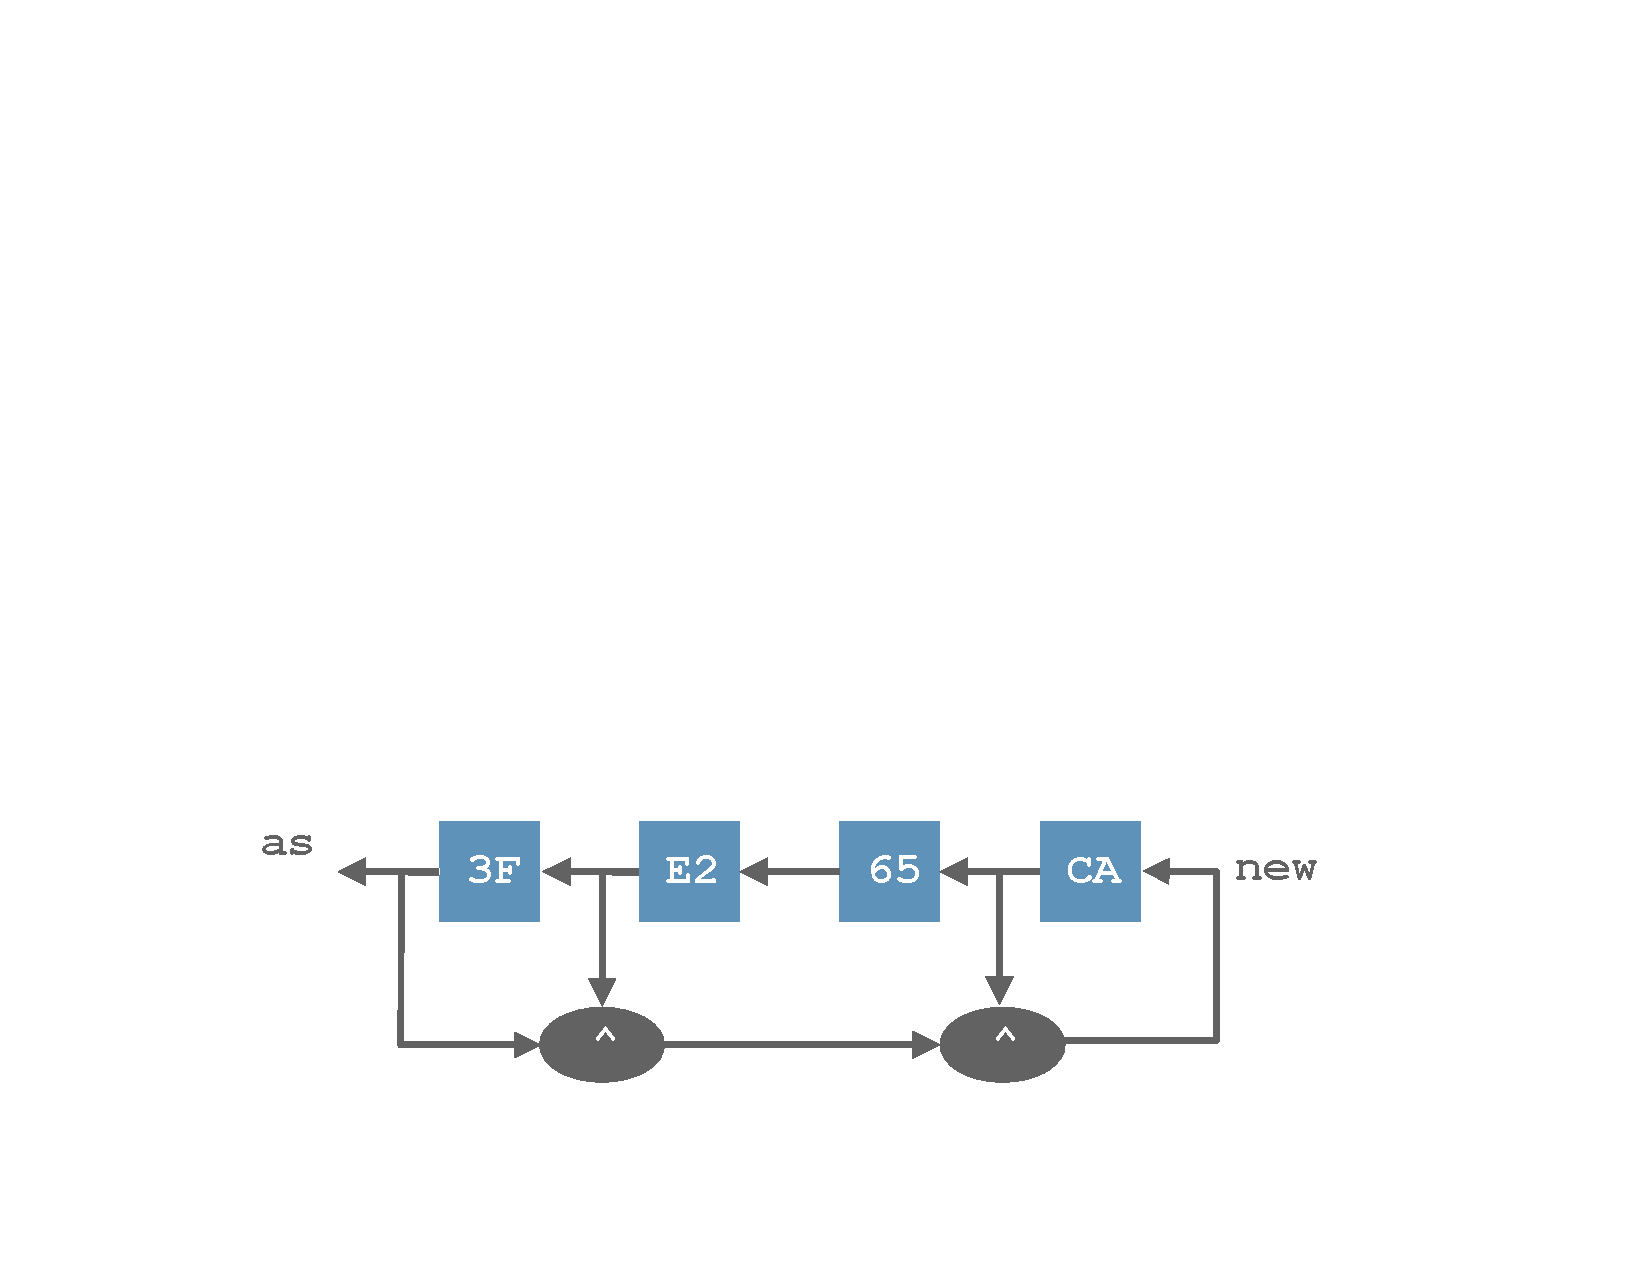
\includegraphics[width=3.5in]{crashCourse/streamDiagram.pdf}
\caption{Equation for producing a stream of {\tt as}}
\label{fig:streamDiagram}
\end{figure}

In this diagram the stream is seeded with four initial values ({\tt
  3F, E2, 65, CA}). The subsequent elements ({\tt new}) are appended
to the stream, and are computed by xor-ing the current stream element
with two additional elements extracted from further into the stream.
The output from the stream is a sequence of values, known as $a$s.

The Cryptol code corresponding to this stream equation is:
\begin{code}
  as  = [0x3F, 0xE2, 0x65, 0xCA] # new
    where
      new = [ a ^ b ^ c | a <- as
                        | b <- drop`{1} as
                        | c <- drop`{3} as ]
\end{code}

% \vfill
% \eject
\todo[inline]{Make sure pagination looks good, particularly for figures.}

\begin{Exercise}\label{ex:streamEq}
  Write the Cryptol code corresponding to the stream equation in
  Figure~\ref{fig:streamExercise}:
\end{Exercise}
\begin{figure}[htbp]
\centering
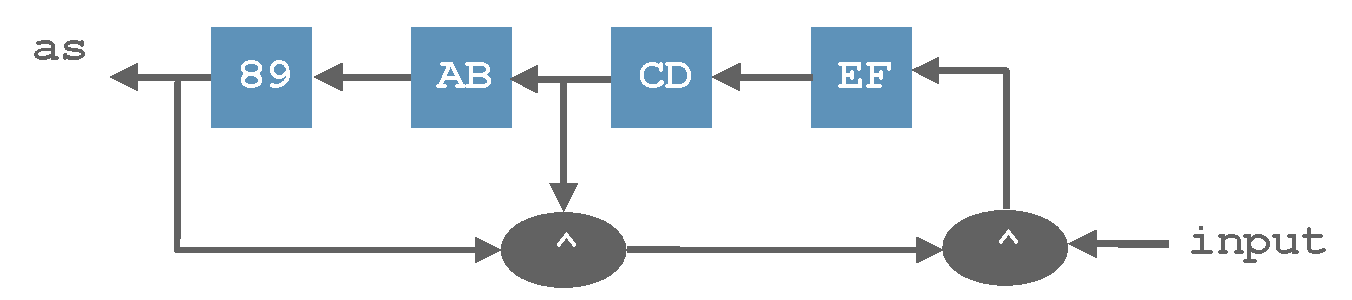
\includegraphics[width=4in]{crashCourse/streamExercise}
\caption{Equation for producing a stream of {\tt as} from an initial
  seed and an input stream.}
\label{fig:streamExercise}
\end{figure}

\todo[inline]{Update diagram so that the output is called \texttt{xs}
  to match the solution and we avoid getting an error from Cryptol
  about redeclaration of \texttt{as}.}

\begin{Answer}\ansref{ex:streamEq}
\begin{code}
  xs input = as where
     as = [0x89, 0xAB, 0xCD, 0xEF] # new
     new = [ a ^ b ^ c | a <- as
                       | b <- drop`{2} as
                       | c <- input ]
\end{code}
\end{Answer}

%=====================================================================
% \section{Type synonyms}
% \label{sec:tsyn}
\sectionWithAnswers{Type synonyms}{sec:tsyn}\indTypSynonym

\todo[inline]{Motivate type synonyms better; NQueens with nice
  synonyms is a good example.}

\todo[inline]{Should we insert a section on currying-style functions
  vs. tuples here?}

Types in Cryptol can become fairly complicated, especially in the
presence of records.  Even for simple types, meaningful names should
be used for readability and documentation.  Type synonyms allow users
to give names to arbitrary types.  In this sense, they are akin to
{\tt typedef} declarations in C~\cite{TheCProgrammingLanguage}.
However, Cryptol's type synonyms are significantly more powerful than
C's {\tt typedef}s, since they can be parameterized by other types,
much like in Haskell~\cite{Has98}.

\todo[inline]{Add a discussion of N-queens or AES or something more compelling
  to show off type synonyms.}

Here are some simple type synonym definitions:
\begin{code}
  type Word8       = [8]
  type CheckedWord = (Word8, Bit)
  type Point a     = {x : [a], y : [a]}
\end{code}

\todo[inline]{2.0: Rewrite this paragraph and much of this section.}

Type synonyms are either unparameterized (as in {\tt Word8} and {\tt
  CheckedWord}, or parameterized with other types (as in {\tt Point}).
Synonyms may depend upon other synonyms, as in the {\tt CheckedWord}
example.  Once the synonym is given, it acts as an additional name for
the underlying type, making it much easier to read and
maintain.

For instance, we can write the function that returns the x-coordinate
of a point as follows:
\begin{code}
  xCoord : {a} Point a -> [a]
  xCoord p = p.x
\end{code}

Type synonyms look like distinct types when they are printed in the
output of the \texttt{:t} and \texttt{:browse} commands. However,
declaring a type synonym does not actually introduce a new
\emph{type}; it merely introduces a new name for an existing type.
When Cryptol's type checker compares types, it expands all type
synonyms first. So as far as Cryptol is concerned, \texttt{Word8} and
\texttt{[8]} are the \emph{same} type. Cryptol preserves type synonyms
in displayed types as a convenience to the user.

For example, consider the following declarations:
%% not "code" to avoid conflicting with previous Word8
\begin{Verbatim}
  type Word8     = [8]
  type Word8'    = [8]
  type B         = Word8
  type A         = B
  type WordPair  = (Word8, Word8')
  type WordPair' = (Word8', Word8)

  foo : Word8 -> Bit
  foo x = True

  bar : Word8' -> Bit
  bar x = foo x
\end{Verbatim}
Within this type context, six different type \emph{names} are
declared, but there are not six distinct \emph{types}. The first four
(\texttt{Word8}, \texttt{Word8'}, \texttt{B}, and \texttt{A}) are all
interchangeable abbreviations for \texttt{[8]}. The last two are
synonymous and interchangeable with the pair type \texttt{([8], [8])}.
Likewise, the function types of \texttt{foo} and \texttt{bar} are
identical, thus \texttt{bar} can call \texttt{foo}.

\begin{Exercise}\label{ex:tsyn:1}
  Define a type synonym for 3-dimensional points and write a function
  to determine if the point lies on any of the 3 axes.
\end{Exercise}
\begin{Answer}\ansref{ex:tsyn:1}
  A point is on the $a^{\text{th}}$ axis if its non-$a^{\text{th}}$
  components are $0$. Hence we have:
\begin{code}
  type Point3D a = {x : [a], y : [a], z : [a]}

  onAnAxis : {a} (fin a) => Point3D a -> Bit
  onAnAxis p = onX || onY || onZ
    where onX = (p.y == 0) && (p.z == 0)
          onY = (p.x == 0) && (p.z == 0)
          onZ = (p.x == 0) && (p.y == 0)
\end{code}
\todo[inline]{Reflect upon this example.}
\end{Answer}

\paragraph*{Predefined type synonyms} The following type synonyms are
predefined in Cryptol:
\begin{Verbatim}
  type Bool = Bit
  type Char = [8]
  type String n = [n]Char
  type Word n = [n]
\end{Verbatim}
For instance, a {\tt String n} is simply a sequence of precisely $n$
8-bit words.\indTSWord\indTSString\indTSBool

\todo[inline]{Discussion of \texttt{String} as a type synonym is an
  important example, so more discussion is warranted.}

%=====================================================================
\section{Type classes}\indTypeClasses
\label{sec:type-classes}

\todo[inline]{This section needs a full rewrite.}

\todo[inline]{Add discussion of Haskell's type classes and other
  typeclass-like things.}

Type classes are a way of describing behaviors shared by multiple
types.  As an example, consider the type of the function {\tt ==}:
\begin{Verbatim}
    Cryptol> :t (==)
    (==) : {a} (Cmp a) => a -> a -> Bit
\end{Verbatim}

This type signature may be read as, ``equality is an operator that
takes two objects of any single type that can be compared and returns
a Bit.''

Cryptol defines a collection of basic type classes: \texttt{Logic},
\texttt{Zero}, \texttt{Cmp}, \texttt{SignedCmp}, \texttt{Arith}, and
\texttt{Literal}. These appear in the type signature of operators and
functions that require them. If a function you define calls, for
example, \texttt{+}, on two arguments both of type \texttt{a}, the
type constraints for \texttt{a} will include \texttt{(Arith a)}.

\begin{itemize}
\item
The \texttt{Logic} typeclass includes the binary logical operators
\texttt{\&\&}, \texttt{||}, and \verb+^+, as well as the unary
operator \verb+~+. Cryptol types made of bits (but not those
containing unbounded integers) are instances of class \texttt{Logic}.

\item
The \texttt{Zero} typeclass includes the special constant
\texttt{zero}. The shifting operators \texttt{<<} and \texttt{>>} are
also in class \texttt{Zero}, because they can shift in zero values.
All of the built-in types of Cryptol are instances of class
\texttt{Zero}.

\item
The \texttt{Cmp} typeclass includes the binary relation operators
\texttt{<}, \texttt{>}, \texttt{<=}, \texttt{>=}, \texttt{==}, and
\texttt{!=}, as well as the binary functions \texttt{min} and
\texttt{max}. Note that equality and other comparisons are bundled
into a single typeclass. Function types are not in class \texttt{Cmp}
and cannot be compared with \texttt{==}, but Cryptol does provide a
special pointwise comparison operator for functions, \texttt{(===) :
  \{a b\} (Cmp b) => (a -> b) -> (a -> b) -> a -> Bit}.

\item
The \texttt{SignedCmp} typeclass includes the binary relation
operators \texttt{<\$}, \texttt{>\$}, \texttt{<=\$}, and
\texttt{>=\$}. These are like \texttt{<}, \texttt{>}, \texttt{<=}, and
\texttt{>=}, except that they interpret bitvectors as \emph{signed}
2's complement numbers, whereas the \texttt{Cmp} operations use the
\emph{unsigned} ordering.

\item
The \texttt{Arith} typeclass includes the binary operators \texttt{+},
\texttt{-}, \texttt{*}, \texttt{/}, \verb+%+, and \verb+^^+, as well
as the unary operators \texttt{lg2} and \texttt{-}, and the function
\texttt{fromInteger}. Infinite sequence enumerations \texttt{[x ...]}
and \texttt{[x, y ...]} are also defined for class \texttt{Arith}.

\item
The \texttt{Literal} typeclass includes numeric literals.
\end{itemize}

\begin{Exercise}\label{ex:tvar:1}
  Without including an explicit type declaration, define a function
  that Cryptol infers has the following type:
\begin{Verbatim}
  cmpArith : {a,b} (Cmp a, Arith b) => a -> a -> b -> b
\end{Verbatim}
\end{Exercise}
\begin{Answer}\ansref{ex:tvar:1}
This code:
\begin{code}
  cmpArith x y z = if x == y then z else z+z
\end{code}
yields the inferred type:
\begin{Verbatim}
  cmpArith : {a, b} (Arith b, Cmp a) => a -> a -> b -> b
\end{Verbatim}
\end{Answer}

%=====================================================================
\section{Type vs.\ value variables}\indTypeVariables
\label{sec:type-vs.-value}

\todo[inline]{Rewrite this whole section to better clarify object- vs. type
  variables, their scope and limitations, where they can be left
  abstract and when and where they must be concretized, etc.}

Its powerful type system is one of the key features of Cryptol. We
have encountered many aspects of types already. You may have noticed,
in functions such as \texttt{split}, that when you call a function in
Cryptol, there are two kinds of parameters you can pass: \textit{value
  variables} and \textit{type variables}.

Consider the \texttt{split} function that we previously examined in
Exercise \autoref{ex:poly:split}. Recall that \texttt{split}'s
type is:
\begin{verbatim}
    split : {parts, each, a} (fin each) =>
              [parts * each]a -> [parts][each]a
\end{verbatim}
When applying \texttt{split}, one typically specifies a concrete
value for the formal parameter \texttt{parts}:
\begin{Verbatim}
    Cryptol> split`{parts=3} [1..12]
    [[1, 2, 3, 4], [5, 6, 7, 8], [9, 10, 11, 12]]
\end{Verbatim}
In this example, the term {\tt\Verb|`{parts=3}|} passes \texttt{3} to
the \texttt{parts} type variable argument, and the \texttt{[1..12]} is
passing a sequence as the first (and only) \textit{value argument}.

A \emph{value variable} is the kind of variable you are used to from
normal programming languages.  This kind of variable represents a
normal run-time value.

A \emph{type variable}, on the other hand, allows you to express
interesting (arithmetic) constraints on \emph{types}. These variables
express things like lengths of sequences or relationships between
lengths of sequences.  Type variable values are computed
statically---they never change at runtime.\footnote{In this way,
  they are similar (but more expressive than) templates in languages
  like C++ or Java. If you want to learn more about this area, look up
  the term ``type-level naturals''.}

%~~~~~~~~~~~~~~~~~~~~~~~~~~~~~~~~~~~~~~~~~~~~~~~~~~~~~~~~~~~~~~~~~~~~~
\subsection{Positional vs.\ named type
  arguments}\indTypePositionalArguments
\label{sec:positional-vs.-named}

Cryptol permits type variables to be passed either by name (as in {\tt
  \Verb|`{parts=3}|} above), or by position (leaving out the name).
For functions you define, the position is the order in which the type
variables are declared in your function's type signature. If you are
not sure what that is, you can always use the {\tt :t} command to find
out the position of type variables.

For example:
\begin{Verbatim}
    Cryptol> :t groupBy
    groupBy : {each, parts, elem}
              (fin each) => [parts * each]elem
                         -> [parts][each]elem
\end{Verbatim}
tells us that that {\tt parts} is in the second position of {\tt
  groupBy}'s type signature, so the positional-style call equivalent
to our example is:
\begin{Verbatim}
    Cryptol> groupBy`{_,3}[1..12]
\end{Verbatim}

Note the use of an underscore in order to pass \texttt{3} in the
second position.  Positional arguments are most often used when the
type argument is the first argument and when the name of the argument
does not add clarity.  The {\tt groupBy\Verb|`{_,3}|} is not as
self-explanatory as {\tt groupBy\Verb|`{parts=3}|}.  On the other hand, our
use of positional arguments to {\tt take} in previous chapters is very
clear, as in:
\begin{Verbatim}
    Cryptol> take`{3}[1..12]
    [1, 2, 3]
\end{Verbatim}

\begin{tip}
  Cryptol programs that use named arguments are more maintainable and
  robust during program evolution.  E.g., you can reorder parameters or
  refactor function definitions much more easily if invocations of
  those functions use named, rather than positional, arguments.
\end{tip}

\todo[inline]{What are the implications to type inference, especially
  resolution, in the presence of positional arguments.}

%~~~~~~~~~~~~~~~~~~~~~~~~~~~~~~~~~~~~~~~~~~~~~~~~~~~~~~~~~~~~~~~~~~~~~
\subsection{Type context vs.\ variable context}\indTypeContext
\label{sec:type-context-vs}

You have seen, in the discussion of type variables above, that Cryptol
has two kinds of variables---type variables and value variables. Type
variables normally show up in type signatures, and value variables
normally show up in function definitions. Sometimes you may want to
use a type variable in a context where value variables would normally
be used.  To do this, use the backtick character {\tt \Verb|`|}.

The definition of the built-in {\tt width} function is a good example
of the use of backtick:
\begin{Verbatim}
    width : {bits, n, a} (fin n, fin bits, bits >= width n) => [n]a -> [bits]
    width _ = `n
\end{Verbatim}

\begin{tip}
  Note there are some subtle things going on in the above definition
  of \texttt{width}.  First, arithmetic constraints on types are
  position-independent; properties of formal parameters early in a
  signature can depend upon those late in a signature.  Second, type
  constraints can refer to not only other functions, but recursively
  to the function that is being defined (either directly, or
  transitively).

  Type constraints can get pretty crazy in practice, especially deep
  in the signature of crypto code subsystems.  Our suggestion is that
  you should not chase the dragon's tail of feedback from the
  typechecker in attempting to massage your specification's types for
  verification.  Instead, think carefully about the meaning and
  purpose of the concepts in your specification, introduce appropriate
  type synonyms, and ensure that the specification is clear and
  precise.  Trust that the interpreter and the verifier will do the
  right thing.
\end{tip}

The bounds in a finite sequence literal (such as \texttt{[1 ..\ 10]}) in
Cryptol are type-level values because the length of a sequence is part
of its type.  Only type-level values can appear in a finite sequence
definition.  You cannot write \texttt{[a ..\ b]} where either \texttt{a} or
\texttt{b} are arguments to a function.  On the other hand, an infinite
sequence's type is fixed (\texttt{[inf]a}), so the initial value in an
infinite sequence can be a runtime variable or a type variable, but
type variables are escaped here using a {\tt \Verb|`|}.

\todo[inline]{Add an example of this here.  Rewrite if something great
  occurs to us.}

\todo[inline]{A proper discussion of type-context vs.~value-context is
  necessary here, and it should be formalized as part of the type
  system and type-inference algorithm, of course.}

This is probably obvious, but there is no way to get a value variable
to appear in a type context.  Types must be known at ``compile time,''
and (non-literal) values are not, so there is no way to use them in
that way.

\todo[inline]{It is more subtle than this because we do not have a proper
  semantic for when arithmetic terms in types (or expressions, for
  that matter!) are evaluated.}

%~~~~~~~~~~~~~~~~~~~~~~~~~~~~~~~~~~~~~~~~~~~~~~~~~~~~~~~~~~~~~~~~~~~~~
\subsection{Inline argument type declarations}\indTypeInline
\label{sec:inline-argument-type}

So far when we have defined a function, we have declared the type of
its arguments and its return value in a separate type declaration.
When you are initially writing code, you might not know exactly what a
function's full type is (including the constraints), but you may know
(and need to express) the types of the function's arguments. Cryptol's
syntax for this should look familiar:
\begin{code}
  addBytes (x:[8]) (y:[8]) = x + y
\end{code}

This defines a function that takes two bytes as input, and returns their sum.
Note that the use of parentheses \texttt{( )} is mandatory.

Here is a more interesting example:
\begin{code}
  myWidth (x:[w]a) = `w
\end{code}

\todo[inline]{Why is this more interesting?  What are the reflections the
  reader should have?}

%=====================================================================
\section{Type constraint synonyms}

Sometimes programs have certain combinations of type constraints that
appear over and over in many places. For convenience, Cryptol allows
the programmer to declare named sets of type constraints that can be
used in other function type signatures. Typically a named type
constraint will have one or more type parameters. The syntax is very
similar to a type synonym declaration:

\begin{code}
  type constraint myConstraint a b = (fin a, fin b, b >= width a)
\end{code}

Wherever a type constraint synonym is used, it is as if its definition
is expanded in place. So the following two signatures would be
equivalent:

\begin{code}
    width : {bits,len,elem} (fin len, fin bits, bits >= width len) =>
            [len] elem -> [bits]
    width : {bits,len,elem} (myConstraint len bits) => [len] elem -> [bits]
\end{code}

%=====================================================================
\section{Program structure with modules}

When a cryptographic specification gets very large it can make sense
to decompose its functions into modules.\indModuleSystem\indImport
Doing this well encourages
code reuse, so it's a generally good thing to do. Cryptol's module
system is simple and easy to use. Here's a quick overview:

A module's name should be the same as the filename the module is
defined in. For example, the \verb+utilities+ module should be
defined in a file called \verb+utilities.cry+. To specify that a file
defines a module, its first non-commented line should be:

\begin{verbatim}
  module utilities where
\end{verbatim}

After that the variables and functions you define will be contained
(in this example) in the {\it utilities} module.

In the code where you want to use a module, you \verb+import+ it like this:
\begin{verbatim}
  import utilities
\end{verbatim}

Cryptol will look for the file \verb+utilities.cry+ in the current directory. Once you've imported a module, all of its variables and functions are available to use in your code.

If you're writing a module that has both {\it private} and {\it public}
definitions, you can hide the ones that shouldn't be exported to modules
that include it by using the \verb+private+ keyword, like this:\indPrivate

\begin{verbatim}
  private internalDouble x = x + x
  exportedDouble = x * 2
\end{verbatim}

As you can tell, by default definitions are exported to including modules.

For a large project it can be convenient to place modules in a directory
structure.  In this case, the directory structure becomes part of the modules'
names.  For example, when placing \verb+SHA3.cry+ in the \verb+Hash+ directory and
accessing it from \verb+HMAC.cry+ you would need to name the modules
accordingly:

\begin{verbatim}

sha3 : {n} (fin n) => [n] -> [512]
sha3 = error "Stubbed, for demonstration only: sha3-512"

blocksize : {n} (fin n, n >= 10) => [n]
blocksize = 576
\end{verbatim}

\begin{verbatim}
module Hash::SHA3 where
import Hash::SHA3

hmac : {keySize, msgSize} (fin keySize, fin msgSize) => [keySize] -> [msgSize] -> [512]
hmac k m = sha3 (ko # sha3 (ki # m))
 where ko    = zipWith (^) kFull (join (repeat 0x5c))
       ki    = zipWith (^) kFull (join (repeat 0x36))
       kFull = if `keySize == blocksize
                 then take (k#zero)
                 else sha3 k
\end{verbatim}

Finally, if you're importing a module that defines something with
a name that you would like to define in your code, you can do a
{\it qualified} import of that module like this:

\begin{verbatim}
  import utilities as util
\end{verbatim}

Now, instead of all the definitions being available in your module,
they are qualified with the name you provided, in this case \verb+util+.
This means you will prefix those names with \verb+util::+ when you call them,
and the unqualified names are able to be defined in your own code.

\begin{verbatim}
  import utilities as util
  // let's say utililities.cry defines "all", and we want to use
  // it in our refined definition of all:
  all xs = util::all xs && (width xs) > 0
\end{verbatim}

%=====================================================================
\section{The road ahead}
\label{sec:road-ahead}

In this introductory chapter, we have seen essentially all of the
language elements in Cryptol. The concepts go deeper, of course, but
you now have enough knowledge to tackle large Cryptol programming
tasks. As with any new language, the more exercises you do, the more
you will feel comfortable with the concepts. In fact, we will take
that point of view in the remainder of this document to walk you
through a number of different examples (both small and large),
employing the concepts we have seen thus far.

%%% Local Variables:
%%% mode: latex
%%% TeX-master: "../main/Cryptol.tex"
%%% End:

\commentout{
\begin{code}
include "../crashCourse/CrashCourse.tex";
\end{code}
}

%%%%%% Transposition ciphers
\commentout{
\begin{code}
  module Classic where
\end{code}
}

\chapter{Classic ciphers}
\label{chapter:classic}

Modern cryptography has come a long way. In his excellent book on
cryptography, Singh traces it back to at least 5th century B.C., to
the times of Herodotus and the ancient Greeks~\cite{Singh:1999:CBE}.
That's some 2500 years ago, and surely we do not use those methods
anymore in modern day cryptography. However, the basic techniques are
still relevant for appreciating the art of secret writing.

Shift ciphers\indShiftcipher construct the \glosCiphertext
ciphertext\indCiphertext from the \glosPlaintext
plaintext\indPlaintext\ by means of a predefined {\em shifting}
operation,\glosCipherkey where the cipherkey of a particular shift
algorithm defines the shift amount of the cipher.\indCipherkey
Transposition ciphers work by keeping the plaintext the same, but {\em
  rearrange} the order of the characters according to a certain rule.
The cipherkey is essentially the description of how this transposition
is done.\indTranspositioncipher Substitution
ciphers\indSubstitutioncipher generalize shifts and transpositions,
allowing one to substitute arbitrary codes for plaintext elements.  In
this chapter, we will study several examples of these techniques and
see how we can code them in Cryptol.

In general, ciphers boil down to pairs of functions \emph{encrypt} and
\emph{decrypt} which ``fit together'' in the appropriate way.  Arguing
that a cryptographic function is \emph{correct} is subtle.

Correctness of cryptography is determined by cryptanalyses by expert
cryptographers.  Each kind of cryptographic primitive (i.e., a hash, a
symmetric cipher, an asymmetric cipher, etc.) has a set of expected
properties, many of which can only be discovered and proven by hand
through a lot of hard work.  Thus, to check the correctness of a
cryptographic function, a best practice for Cryptol use is to encode
as many of these properties as one can in Cryptol itself and use
Cryptol's validation and verification capabilities, discussed
later in~\autoref{cha:high-assur-progr}.  For example, the fundamental
property of most ciphers is that encryption and decryption are
inverses of each other.

To check the correctness of an \emph{implementation} $I$ of a
cryptographic function $C$ means that one must show that the
implementation $I$ behaves as the specification ($C$) stipulates.  In
the context of cryptography, the minimal conformance necessary is
that $I$'s output \emph{exactly} conforms to the output characterized
by $C$.  But just because a cryptographic implementation is
\emph{functionally correct} does not mean it is \emph{secure}.  The
subtleties of an implementation can leak all kinds of information that
harm the security of the cryptography, including abstraction leaking
of sensitive values, timing attacks, side-channel attacks, etc.  These
kinds of properties cannot currently be expressed or reasoned about in
Cryptol.

Also, Cryptol does \emph{not} give the user any feedback on the
\emph{strength} of a given (cryptographic) algorithm.  While this is
an interesting and useful feature, it is not part of Cryptol's current
capabilities.

%=====================================================================
% \section{Caesar's cipher}
% \label{sec:caesar}
\sectionWithAnswers{Caesar's cipher}{sec:caesar}

Caesar's cipher (a.k.a. Caesar's shift) is one of the simplest
ciphers.  The letters in the plaintext\indPlaintext are shifted by a
fixed number of elements down the alphabet.\indCaesarscipher For
instance, if the shift is 2, {\tt A} becomes {\tt C}, {\tt B} becomes
{\tt D}, and so on. Once we run out of letters, we circle back to {\tt
  A}; so {\tt Y} becomes {\tt A}, and {\tt Z} becomes {\tt B}.  Coding
Caesar's cipher in Cryptol is quite straightforward (recall from
Section~\ref{sec:tsyn} that a {\tt String n} is simply a sequence of n
8-bit words.):\indTSString
\begin{code}
  caesar : {n} ([8], String n) -> String n
  caesar (s, msg) = [ shift x | x <- msg ]
        where map     = ['A' .. 'Z'] <<< s
              shift c = map @ (c - 'A')
\end{code}
In this definition, we simply get a message {\tt msg} of type {\tt
  String n}, and perform a {\tt shift} operation on each one of the
elements.  The {\tt shift} function is defined locally in the {\tt
  where}-clause.\indWhere To compute the shift, we first find the
distance of the letter from the character {\tt 'A'} (via {\tt c -
  'A'}), and look it up in the mapping imposed by the shift. The {\tt
  map} is simply the alphabet rotated to the left by the shift amount,
{\tt s}. Note how we use the enumeration {\tt ['A' .. 'Z']} to get all
the letters in the alphabet.\indEnum

\begin{Exercise}\label{ex:caesar:0}
  What is the map corresponding to a shift of 2? Use Cryptol's
  \verb+<<<+\indRotLeft to compute it.  You can use the command {\tt
    :set ascii=on}\indSettingASCII to print strings in ASCII, like
  this:
\begin{Verbatim}
  Cryptol> :set ascii=on
  Cryptol> "Hello World"
  "Hello World"
\end{Verbatim}
Why do we use a left-rotate, instead of a right-rotate?
\end{Exercise}
\begin{Answer}\ansref{ex:caesar:0}
Here is the alphabet and the corresponding shift-2 Caesar's alphabet:
\begin{verbatim}
  Cryptol> ['A'..'Z'] 
  "ABCDEFGHIJKLMNOPQRSTUVWXYZ"
  Cryptol> ['A'..'Z'] <<< 2
  "CDEFGHIJKLMNOPQRSTUVWXYZAB"
\end{verbatim}
We use a left rotate to get the characters lined up correctly, as
illustrated above.  \indRotLeft\indRotRight
\end{Answer}

\begin{Exercise}\label{ex:caesar:1}
  Use the above definition to encrypt the message {\tt "ATTACKATDAWN"}
  by shifts 0, 3, 12, and 52. What happens when the shift is a
  multiple of 26? Why?
\end{Exercise}
\begin{Answer}\ansref{ex:caesar:1}
Here are Cryptol's responses:
\begin{Verbatim}
  Cryptol> caesar (0, "ATTACKATDAWN")
  "ATTACKATDAWN"
  Cryptol> caesar (3, "ATTACKATDAWN")
  "DWWDFNDWGDZQ"
  Cryptol> caesar (12, "ATTACKATDAWN")
  "MFFMOWMFPMIZ"
  Cryptol> caesar (52, "ATTACKATDAWN")
  "ATTACKATDAWN"
\end{Verbatim}
If the shift is a multiple of 26 (as in 0 and 52 above), the letters
will cycle back to their original values, so encryption will leave the
message unchanged. Users of the Caesar's cipher should be careful
about picking the shift amount!
\end{Answer}

\begin{Exercise}\label{ex:caesar:2}
  Write a function {\tt dCaesar} which will decrypt a ciphertext
  constructed by a Caesar's cipher. It should have the same signature
  as {\tt caesar}.  Try it on the examples from the previous exercise.
\end{Exercise}
\begin{Answer}\ansref{ex:caesar:2}
  The code is almost identical, except we need to use a right
  rotate:\indRotRight

\begin{code}
  dCaesar : {n} ([8], String n) -> String n
  dCaesar (s, msg) = [ shift x | x <- msg ]
        where map     = ['A' .. 'Z'] >>> s
              shift c = map @ (c - 'A')
\end{code}
%  dCaesar : {n} ([8], String n) -> String n
%  dCaesar (s, msg) = [ shift x | x <- msg ]
%    where  map     = ['A' .. 'Z']  >>> s
%           shift c = map @ (c - 'A')
We have:
\begin{Verbatim}
  Cryptol> caesar (12, "ATTACKATDAWN")
  "MFFMOWMFPMIZ"
  Cryptol> dCaesar (12, "MFFMOWMFPMIZ")
  "ATTACKATDAWN"
\end{Verbatim}
\end{Answer}

\begin{Exercise}\label{ex:caesar:3}
  Observe that the shift amount in a Caesar cipher is very limited:
  Any shift of {\tt d} is equivalent to a shift by {\tt d \% 26}. (For
  instance shifting by 12 and 38 is the same thing, due to wrap around
  at 26.) Based on this observation, how strong do you think the
  Caesar's cipher is? Describe a simple attack that will recover the
  plaintext and automate it using Cryptol.  Use your function to crack
  the ciphertext {\tt JHLZHYJPWOLYPZDLHR}.
\end{Exercise}
\begin{Answer}\ansref{ex:caesar:3}
  For the Caesar's cipher, the only good shifts are $1$ through $25$,
  since shifting by $0$ would return the plaintext unchanged, and any
  shift amount {\tt d} that is larger than $26$ and over is essentially
  the same as shifting by {\tt d \% 26} due to wrap around. Therefore,
  all it takes to break the Caesar cipher is to try the sizes $1$
  through $25$, and see if we have a valid message. We can automate this
  in Cryptol by returning all possible plaintexts using these shift
  amounts:
\begin{code}
  attackCaesar : {n} (String n) -> [25](String n)
  attackCaesar msg = [ dCaesar(i, msg) | i <- [1 .. 25] ]
\end{code}
If we apply this function to {\tt JHLZHYJPWOLYPZDLHR}, we get:
\begin{Verbatim}
  Cryptol> :set ascii=on
  Cryptol> attackCaesar "JHLZHYJPWOLYPZDLHR",
  ["IGKYGXIOVNKXOYCKGQ", "HFJXFWHNUMJWNXBJFP", "GEIWEVGMTLIVMWAIEO"
   "FDHVDUFLSKHULVZHDN", "ECGUCTEKRJGTKUYGCM", "DBFTBSDJQIFSJTXFBL"
   "CAESARCIPHERISWEAK", "BZDRZQBHOGDQHRVDZJ", "AYCQYPAGNFCPGQUCYI"
   "ZXBPXOZFMEBOFPTBXH", "YWAOWNYELDANEOSAWG", "XVZNVMXDKCZMDNRZVF"
   "WUYMULWCJBYLCMQYUE", "VTXLTKVBIAXKBLPXTD", "USWKSJUAHZWJAKOWSC"
   "TRVJRITZGYVIZJNVRB", "SQUIQHSYFXUHYIMUQA", "RPTHPGRXEWTGXHLTPZ"
   "QOSGOFQWDVSFWGKSOY", "PNRFNEPVCUREVFJRNX", "OMQEMDOUBTQDUEIQMW"
   "NLPDLCNTASPCTDHPLV", "MKOCKBMSZROBSCGOKU", "LJNBJALRYQNARBFNJT"
   "KIMAIZKQXPMZQAEMIS"]
\end{Verbatim}
If you skim through the potential ciphertexts, you will see that the
$7^{th}$ entry is probably the one we are looking for. Hence the key
must be $7$.  Indeed, the message is {\tt CAESARCIPHERISWEAK}.
\end{Answer}

\begin{Exercise}\label{ex:caesar:4}
  One classic trick to strengthen ciphers is to use multiple keys. By
  repeatedly encrypting the plaintext multiple times we can hope that
  it will be more resistant to attacks. Do you think this scheme might
  make the Caesar cipher stronger?
\end{Exercise}
\begin{Answer}\ansref{ex:caesar:4}
  No. Using two shifts $d_1$ and $d_2$ is essentially the same as
  using just one shift with the amount $d_1 + d_2$. Our attack
  function would work just fine on this schema as well. In fact, we
  wouldn't even have to know how many rounds of encryption was
  applied. Multiple rounds is just as weak as a single round when it
  comes to breaking the Caesar's cipher.  \end{Answer}

\begin{Exercise}\label{ex:caesar:5}
  What happens if you pass {\tt caesar} a plaintext that has
  non-uppercase letters in it? (Let's say a digit.) How can you fix
  this deficiency?
\end{Exercise}
\begin{Answer}\ansref{ex:caesar:5}
In this case we will fail to find a mapping:
\begin{Verbatim}
  Cryptol> caesar (3, "12")
  ... index of 240 is out of bounds
  (valid range is 0 thru 25).
\end{Verbatim}
What happened here is that Cryptol computed the offset {\tt '1' - 'A'}
to obtain the $8$-bit index $240$ (remember, modular arithmetic!), but
our alphabet only has $26$ entries, causing the out-of-bounds error.
\todo[inline]{Say something about how to guarantee that such errors
  are impossible. (Use of preconditions, checking and proving safety,
  etc.)}  We can simply remedy this problem by allowing our alphabet
to contain all $8$-bit numbers:\indRotLeft
\begin{code}
  caesar' : {n} ([8], String n) -> String n
  caesar' (s, msg) = [ shift x | x <- msg ]
    where map     = [0 .. 255] <<< s
          shift c = map @ c
\end{code}
Note that we no longer have to subtract {\tt 'A'}, since we are
allowing a much wider range for our plaintext and ciphertext. (Another
way to put this is that we are subtracting the value of the first
element in the alphabet, which happens to be 0 in this case!
Consequently, the number of ``good'' shifts increase from $25$ to
$255$.)  The change in {\tt dCaesar'} is analogous:\indRotRight
\begin{code}
  dCaesar' : {n} ([8], String n) -> String n
  dCaesar' (s, msg) = [ shift x | x <- msg ]
    where  map     = [0 .. 255] >>> s
           shift c = map @ c
\end{code}
\end{Answer}

%=====================================================================
% \section{\texorpdfstring{Vigen\`{e}re}{Vigenere} cipher}
% \label{sec:vigenere}
\sectionWithAnswers{\texorpdfstring{Vigen\`{e}re}{Vigenere} cipher}{sec:vigenere}

The Vigen\`{e}re cipher is a variation on the Caesar's cipher, where
one uses multiple shift amounts according to a
keyword~\cite{wiki:vigenere}.\indVigenere Despite its simplicity, it
earned the notorious description {\em le chiffre ind\`{e}chiffrable}
(``the indecipherable cipher'' in French), as it was unbroken for a
long period of time. It was very popular in the 16th century and
onwards, only becoming routinely breakable by mid-19th century or so.

To illustrate the operation of the Vigen\`{e}re cipher, let us
consider the plaintext {\tt ATTACKATDAWN}. The cryptographer picks a
key, let's say {\tt CRYPTOL}. We line up the plaintext and the key,
repeating the key as much as as necessary, as in the top two lines of
the following:
\begin{tabbing}
\hspace*{2cm} \= Ciphertext: \hspace*{.5cm} \= {\tt CKRPVYLVUYLG} \kill 
\> Plaintext : \> {\tt ATTACKATDAWN} \\
\> Cipherkey : \> {\tt CRYPTOLCRYPT} \\
\> Ciphertext: \> {\tt CKRPVYLVUYLG}
\end{tabbing}
We then proceed pair by pair, shifting the plaintext character by the
distance implied by the corresponding key character.  The first pair
is {\tt A}-{\tt C}.  Since {\tt C} is two positions away from {\tt A}
in the alphabet, we shift {\tt A} by two positions, again obtaining
{\tt C}.  The second pair {\tt T}-{\tt R} proceeds similarly: Since
{\tt R} is 17 positions away from {\tt A}, we shift {\tt T} down 17
positions, wrapping around {\tt Z}, obtaining {\tt K}.  Proceeding in
this fashion, we get the ciphertext {\tt CKRPVYLVUYLG}. Note how each
step of the process is a simple application of the Caesar's
cipher.\indCaesarscipher

\begin{Exercise}\label{ex:vigenere:0}
  One component of the Vigen\`{e}re cipher is the construction of the
  repeated key.  Write a function {\tt cycle} with the following
  signature:
\begin{code}
  cycle : {n, a} (fin n, n >= 1) => [n]a -> [inf]a
\end{code}
such that it returns the input sequence appended to itself repeatedly,
turning it into an infinite sequence. Why do we need the predicate
{\tt n >= 1}?\indPredicates
\end{Exercise}
\begin{Answer}\ansref{ex:vigenere:0}
Here is one way to define {\tt cycle}, using a recursive definition:
\begin{code}
  cycle xs = xss
        where xss = xs # xss
\end{code}
We have:
\begin{Verbatim}
  Cryptol> cycle [1 .. 3]
  [1, 2, 3, 1, 2, ...]
\end{Verbatim}
If we do not have the {\tt n >= 1} predicate, then we can pass {\tt
  cycle} the empty sequence, which would cause an infinite loop
emitting nothing.  The predicate {\tt n >= 1} makes sure the input is
non-empty, guaranteeing that {\tt cycle} can produce the infinite
sequence.
\end{Answer}

\begin{Exercise}\label{ex:vigenere:1}
  Program the Vigen\`{e}re cipher in Cryptol. It should have the
  signature:
\begin{code}
  vigenere : {n, m} (fin n, n >= 1) => (String n, String m) -> String m
\end{code}
where the first argument is the key and the second is the
plaintext. Note how the signature ensures that the input string and
the output string will have precisely the same number of characters,
{\tt m}. \lhint{Use Caesar's cipher repeatedly.}
\end{Exercise}
\begin{Answer}\ansref{ex:vigenere:1}
\begin{code}
  vigenere (key, pt) = join [ caesar (k - 'A', [c]) 
                              | c <- pt
                              | k <- cycle key
                            ]
\end{code}
Note the shift is determined by the distance from the letter {\tt 'A'}
for each character. Here is the cipher in action:
\begin{Verbatim}
  Cryptol> vigenere ("CRYPTOL", "ATTACKATDAWN")
  "CKRPVYLVUYLG"
\end{Verbatim}
\end{Answer}

\begin{Exercise}\label{ex:vigenere:2}
  Write the decryption routine for Vigen\`{e}re. Then decode \\
  {\tt "XZETGSCGTYCMGEQGAGRDEQC"} with the key {\tt "CRYPTOL"}.
\end{Exercise}
\begin{Answer}\ansref{ex:vigenere:2}
Following the lead of the encryption, we can rely on {\tt dCaesar}:
\begin{code}
  dVigenere : {n, m} (fin n, n >= 1) => 
              (String n, String m) -> String m
  dVigenere (key, pt) = join [ dCaesar (k - 'A', [c]) 
                               | c <- pt
                               | k <- cycle key
                             ]
\end{code}
The secret code is:
\begin{Verbatim}
  Cryptol> dVigenere ("CRYPTOL", "XZETGSCGTYCMGEQGAGRDEQC")
  "VIGENERECANTSTOPCRYPTOL"
\end{Verbatim}
\end{Answer}

\begin{Exercise}\label{ex:vigenere:3}
  A known-plaintext attack\indKnownPTAttack is one where an attacker
  obtains a plaintext-ciphertext pair, without the key. If the
  attacker can figure out the key based on this pair then he can break
  all subsequent communication until the key is replaced. Describe how
  one can break the Vigen\`{e}re cipher if a plaintext-ciphertext pair
  is known.
\end{Exercise}
\begin{Answer}\ansref{ex:vigenere:3}
  All it takes is to decrypt using using the plaintext as the key and
  message as the cipherkey. Here is this process in action. Recall
  from the previous exercise that encrypting {\tt ATTACKATDAWN} by the
  key {\tt CRYPTOL} yields {\tt CKRPVYLVUYLG}. Now, if an attacker
  knows that {\tt ATTACKATDAWN} and {\tt CKRPVYLVUYLG} form a pair,
  he/she can find the key simply by:\indVigenere
\begin{Verbatim}
  Cryptol> dVigenere ("ATTACKATDAWN", "CKRPVYLVUYLG")
  "CRYPTOLCRYPT"
\end{Verbatim}
Note that this process will not always tell us what the key is
precisely.  It will only be the key repeated for the given message
size. For sufficiently large messages, or when the key does not repeat
any characters, however, it would be really easy for an attacker to
glean the actual key from this information.

This trick works since the act of using the plaintext as the key and
the ciphertext as the message essentially reverses the shifting
process, revealing the shift amounts for each pair of characters.  The
same attack would essentially work for the Caesar's cipher as well,
where we would only need one character to crack it.\indCaesarscipher
\end{Answer}

%%%% Way too complicated for the intro.. skipping for now
%% \section{Rail fence cipher}
%% \lable{sec:railfence}
%% \sectionWithAnswers{Rail fence cipher}{sec:railfence}\indRailFence
%% The $k$-rail fence cipher is a simple example of a transposition
%% cipher\indTranspositioncipher, where the text is written along {\em
%% k}-lines in a zig-zag fashion. For instance, to encrypt {\tt
%% ATTACKATDAWN} using a 3-rail fence, we construct the following
%% text:
%% \begin{Verbatim}
%%  A . . . C . . . D . . .
%% . T . A . K . T . A . N
%% . . T . . . A . . . W .
%% \end{Verbatim}
%% going down and up the 3 fences in a zigzag fashion. We then read
%% the ciphertext\indCiphertext line by line to obtain:
%% \begin{Verbatim}
%%   ACDTAKTANTAW
%% \end{Verbatim}
%% 
%% \begin{Exercise}\label{ex:railfence:0}
%%   Program the 3-rail fence cipher in Cryptol. You should write the
%%   functions:
%% \begin{code}
%%   rail3Fence, dRail3Fence : {a} (fin a) => String((4*a))  -> String ((4*a));
%% \end{code}
%% that implements the 3-rails encryption/decryption. Using your
%% functions, encrypt and decrypt the message {\tt
%% RAILFENCECIPHERISTRICKIERTHANITLOOKS}.
%% \end{Exercise}
%% \begin{Answer}\ansref{ex:railfence:0}
%% \begin{code}
%%   rail3Fence pt = heads # mids # tails
%%   where {
%%      regions = groupBy (4, pt);
%%      heads   =      [| r @ 0             || r <- regions |];
%%      mids    = join [| [(r @ 1) (r @ 3)] || r <- regions |];
%%      tails   =      [| r @ 2             || r <- regions |];
%%   };
%% \end{code}
%% \end{Answer}

%=====================================================================
% \section{The atbash}
% \label{sec:atbash}
\sectionWithAnswers{The atbash}{sec:atbash}

The atbash cipher is a form of a shift cipher, where each letter is
replaced by the letter that occupies its mirror image position in the
alphabet.\indAtbash That is, {\tt A} is replaced by {\tt Z}, {\tt B}
by {\tt Y}, etc. Needless to say the atbash is hardly worthy of
cryptographic attention, as it is trivial to break.

\begin{Exercise}\label{ex:atbash:0}
  Program the atbash in Cryptol. What is the code for {\tt
    ATTACKATDAWN}?
\end{Exercise}
\begin{Answer}\ansref{ex:atbash:0}
  Using the reverse index operator, coding atbash is
  trivial:\indRIndex\indAtbash
\begin{code}
  atbash : {n} String n -> String n
  atbash pt = [ alph ! (c - 'A') | c <- pt ]
      where alph = ['A' .. 'Z']
\end{code}
We have:
\begin{Verbatim}
  Cryptol> atbash "ATTACKATDAWN"
  "ZGGZXPZGWZDM"
\end{Verbatim}
\end{Answer}

\begin{Exercise}\label{ex:atbash:1}
  Program the atbash decryption in Cryptol. Do you have to write any
  code at all? Break the code {\tt ZGYZHSRHHVOUWVXIBKGRMT}.
\end{Exercise}
\begin{Answer}\ansref{ex:atbash:1}
  Notice that decryption for atbash\indAtbash is precisely the same as
  encryption, the process is entirely the same. So, we do not have to
  write any code at all, we can simply define:
\begin{code}
  dAtbash : {n} String n -> String n
  dAtbash = atbash
\end{code}
We have:
\begin{Verbatim}
  Cryptol> dAtbash "ZGYZHSRHHVOUWVXIBKGRMT"
  "ATBASHISSELFDECRYPTING"
\end{Verbatim}
\end{Answer}

%=====================================================================
% \section{Substitution ciphers}
% \label{section:subst}
\sectionWithAnswers{Substitution ciphers}{section:subst}

Substitution ciphers\indSubstitutioncipher generalize all the ciphers
we have seen so far, by allowing arbitrary substitutions to be made
for individual ``components'' of the
plaintext~\cite{wiki:substitution}.  Note that these components need
not be individual characters, but rather can be pairs or even triples
of characters that appear consecutively in the text. (The
multi-character approach is termed {\em
  polygraphic}.)\indPolyGraphSubst Furthermore, there are variants
utilizing multiple {\em polyalphabetic} mappings,\indPolyAlphSubst as
opposed to a single {\em monoalphabetic} mapping\indMonoAlphSubst.  We
will focus on monoalphabetic simple substitutions, although the other
variants are not fundamentally more difficult to implement.

\tip{For the exercises in this section we will use a running key
  repeatedly. To simplify your interaction with Cryptol, put the
  following definition in your program file:}
\begin{code}
  substKey : String 26
  substKey = "FJHWOTYRXMKBPIAZEVNULSGDCQ"
\end{code}
The intention is that {\tt substKey} maps {\tt A} to {\tt F}, {\tt B}
to {\tt J}, {\tt C} to {\tt H}, and so on.

\begin{Exercise}\label{ex:subst:0}
  Implement substitution ciphers in Cryptol. Your function should have
  the signature:
\begin{code}
  subst : {n} (String 26, String n) -> String n
\end{code}
where the first element is the key (like {\tt substKey}).
What is the code for \\
{\tt "SUBSTITUTIONSSAVETHEDAY"} for the key {\tt substKey}?
\end{Exercise}
\begin{Answer}\ansref{ex:subst:0}
\begin{code}
  subst (key, pt) = [ key @ (p - 'A') | p <- pt ]
\end{code}
We have:
\begin{Verbatim}
  Cryptol> subst(substKey, "SUBSTITUTIONSSAVETHEDAY")
  "NLJNUXULUXAINNFSOUROWFC"
\end{Verbatim}
\end{Answer}

\paragraph*{Decryption} Programming decryption is more subtle.  We can
no longer use the simple selection operation ({\tt @})\indIndex on the
key. Instead, we have to search for the character that maps to the
given ciphertext character.

\begin{Exercise}\label{ex:subst:1}
Write a function {\tt invSubst} with the following signature:
%%   type Char = [8] // now in prelude.cry
\begin{code}
  invSubst : (String 26, Char) -> Char
\end{code}
such that it returns the mapped plaintext character. For instance,
with {\tt substKey}, {\tt F} should get you {\tt A}, since the key
maps {\tt A} to {\tt F}:
\begin{Verbatim}
  Cryptol> invSubst (substKey, 'F')
  A
\end{Verbatim}
And similarly for other examples:
\begin{Verbatim}
  Cryptol> invSubst (substKey, 'J')
  B
  Cryptol> invSubst (substKey, 'C')
  Y
  Cryptol> invSubst (substKey, 'Q')
  Z
\end{Verbatim}
One question is what happens if you search for a non-existing
character.  In this case you can just return {\tt 0}, a non-valid
ASCII character, which can be interpreted as {\em not found}.
\hint{Use a fold (see Pg.~\pageref{par:fold}).}\indFold
\end{Exercise}
\begin{Answer}\ansref{ex:subst:1}
\begin{code}
  invSubst (key, c) = candidates ! 0
    where candidates = [0] # [ if c == k then a else p
                             | k <- key
                             | a <- ['A' .. 'Z']
                             | p <- candidates
                             ]
\end{code}
The comprehension\indComp defining {\tt candidates} uses a fold (see
page~\pageref{par:fold}).\indFold The first branch ({\tt k <- key})
walks through all the key elements, the second branch walks through
the ordinary alphabet ({\tt a <- ['A' .. 'Z']}), and the final branch
walks through the candidate match so far. At the end of the fold, we
simply return the final element of {\tt candidates}. Note that we
start with {\tt 0} as the first element, so that if no match is found
we get a {\tt 0} back.
\end{Answer}

\begin{Exercise}\label{ex:subst:2}
  Using {\tt invSubst}, write the decryption function {\tt dSubst}.
  It should have the exact same signature as {\tt subst}.  Decrypt
  {\tt FUUFHKFUWFGI}, using our running key.
\end{Exercise}
\begin{Answer}\ansref{ex:subst:2}
\begin{code}
  dSubst: {n} (String 26, String n) -> String n
  dSubst (key, ct) = [ invSubst (key, c) | c <- ct ]
\end{code}
We have:
\begin{Verbatim}
  Cryptol> dSubst (substKey, "FUUFHKFUWFGI")
  "ATTACKATDAWN"
\end{Verbatim}
\end{Answer}

\todo[inline]{This exercise and the true type of \texttt{invSubst}
  indicate that specs are needed.  In other words, we cannot capture
  \texttt{invSubst}'s tightest type, which would encode the invariant
  about contents being capital letters, and that lack of
  expressiveness leaks to \texttt{dSubst}.  We really need to either
  enrich the dependent types or add some kind of support for
  contracts.  The reason this works most of the time is that crypto
  algorithms work on arbitrary bytes.}

\begin{Exercise}\label{ex:subst:3}
  Try the substitution cipher with the key {\tt
    AAAABBBBCCCCDDDDEEEEFFFFGG}. Does it still work?  What is special
  about {\tt substKey}?
\end{Exercise}
\begin{Answer}\ansref{ex:subst:3}
No, with this key we cannot decrypt properly:
\begin{Verbatim}
  Cryptol> subst ("AAAABBBBCCCCDDDDEEEEFFFFGG", "HELLOWORLD")
  "BBCCDFDECA"
  Cryptol> dSubst ("AAAABBBBCCCCDDDDEEEEFFFFGG", "BBCCDFDECA")
  "HHLLPXPTLD"
\end{Verbatim}
This is because the given key maps multiple plaintext letters to the
same ciphertext letter. (For instance, it maps all of {\tt A}, {\tt
  B}, {\tt C}, and {\tt D} to the letter {\tt A}.) For substitution
ciphers to work the key should not repeat the elements, providing a
1-to-1 mapping. This property clearly holds for {\tt substKey}. Note
that there is no shortage of keys, since for 26 letters we have 26!
possible ways to choose keys, which gives us over 4-billion different
choices.
\end{Answer}

%=====================================================================
% \section{The scytale}
% \label{sec:scytale}
\sectionWithAnswers{The scytale}{sec:scytale}

The scytale is one of the oldest cryptographic devices ever, dating
back to at least the first century
A.D.~\cite{wiki:scytale}.\indScytale Ancient Greeks used a leather
strip on which they would write their plaintext\indPlaintext message.
The strip would be wrapped around a rod of a certain diameter. Once
the strip is completely wound, they would read the text row-by-row,
essentially transposing the letters and constructing the
ciphertext\indCiphertext. Since the ciphertext is formed by a
rearrangement of the plaintext, the scytale is an example of a
transposition cipher.\indTranspositioncipher To decrypt, the
ciphertext needs to be wrapped around a rod of the same diameter,
reversing the process. The cipherkey\indCipherkey is essentially the
diameter of the rod used. Needless to say, the scytale does not
provide a very strong encryption mechanism.

Abstracting away from the actual rod and the leather strip, encryption
is essentially writing the message column-by-column in a matrix and
reading it row-by-row.  Let us illustrate with the message {\tt
  ATTACKATDAWN}, where we can fit 4 characters per column:
\begin{verbatim}
    ACD
    TKA
    TAW
    ATN
\end{verbatim}
To encrypt, we read the message row-by-row, obtaining {\tt
  ACDTKATAWATN}. If the message does not fit properly (i.e., if it has
empty spaces in the last column), it can be padded by {\tt Z}'s or
some other agreed upon character. To decrypt, we essentially reverse
the process, by writing the ciphertext row-by-row and reading it
column-by-column.

Notice how the scytale's operation is essentially matrix
transposition.  Therefore, implementing the scytale in Cryptol is
merely an application of the {\tt transpose} function.\indTranspose
All we need to do is group the message by the correct number of
elements using {\tt split}.\indSplit Below, we define the {\tt
  diameter} to be the number of columns we have. The type synonym {\tt
  Message} ensures we only deal with strings that properly fit the
``rod,'' by using {\tt r} number of rows:\indJoin

\begin{code}
  scytale : {row, diameter} (fin row, fin diameter)
            => String (row * diameter) -> String (diameter * row)
  scytale msg = join (transpose msg')
       where   msg' : [diameter][row][8]
               msg' = split msg
\end{code}
The signature\indSignature on {\tt msg'} is revealing: We are taking a
string that has {\tt diameter * row} characters in it, and chopping it
up so that it has {\tt row} elements, each of which is a string that
has {\tt diameter} characters in it.  Here is Cryptol in action,
encrypting the message {\tt ATTACKATDAWN}:
\begin{Verbatim}
  Cryptol> :set ascii=on
  Cryptol> scytale "ATTACKATDAWN"
  "ACDTKATAWATN"
\end{Verbatim}
Decryption is essentially the same process, except we have to {\tt
  split} so that we get {\tt diameter} elements
out:\indSplit\indJoin\indScytale
\begin{code}
  dScytale : {row, diameter} (fin row, fin diameter) 
             => String (row * diameter) -> String (diameter * row)
  dScytale msg = join (transpose msg')
     where   msg' : [row][diameter][8]
             msg' = split msg
\end{code}
Again, the type on {\tt msg'} tells Cryptol that we now want {\tt
  diameter} strings, each of which is {\tt row} long.  It is important
to notice that the definitions of {\tt scytale} and {\tt dScytale} are
precisely the same, except for the signature on {\tt msg'}! When
viewed as a matrix, the types precisely tell which transposition we
want at each step.  We have:
\begin{Verbatim}
  Cryptol> dScytale "ACDTKATAWATN"
  "ATTACKATDAWN"
\end{Verbatim}

\begin{Exercise}\label{ex:scytale:0}
  What happens if you comment out the signature for {\tt msg'} in the
  definition of {\tt scytale}? Why?\indScytale
\end{Exercise}
\begin{Answer}\ansref{ex:scytale:0}
  If you do not provide a signature for {\tt msg'}, you will get the
  following type-error message from Cryptol:
\begin{small}
\begin{Verbatim}
  Failed to validate user-specified signature.
    In the definition of 'scytale', at classic.cry:40:1--40:8:
      for any type row, diameter
        fin row
        fin diameter
      =>
      fin ?b
        arising from use of expression split at classic.cry:42:17--42:22
      fin ?d
        arising from use of expression join at classic.cry:40:15--40:19
      row * diameter == ?a * ?b
        arising from matching types at classic.cry:1:1--1:1
\end{Verbatim}
\end{small}
Essentially, Cryptol is complaining that it was asked to do a {\tt
  split}\indSplit and it figured that the constraint
$\text{\emph{diameter}}*\text{\emph{row}}=a*b$ must hold, but that is
not sufficient to determine what {\tt a} and {\tt b} should really
be. (There could be multiple ways to assign {\tt a} and {\tt b} to
satisfy that requirement, for instance {\tt a=4}, {\tt b=row}; or {\tt
  a=2} and {\tt b=2*row}, resulting in differing behavior.)  This is
why it is unable to ``validate the user-specified signature''.  By
putting the explicit signature for {\tt msg'}, we are giving Cryptol
more information to resolve the ambiguity. Notice that since the code
for {\tt scytale} and {\tt dScytale} are precisely the same except for
the type on {\tt msg'}. This is a clear indication that the type
signature plays an essential role here.\indAmbiguity\indSignature
\end{Answer}

\begin{Exercise}\label{ex:scytale:1}
  How would you attack a scytale encryption, if you don't know what
  the diameter is?
\end{Exercise}
\begin{Answer}\ansref{ex:scytale:1}
  Even if we do not know the diameter, we do know that it is a divisor
  of the length of the message. For any given message size, we can
  compute the number of divisors of the size and try decryption until
  we find a meaningful plaintext.  Of course, the number of potential
  divisors will be large for large messages, but the practicality of
  scytale stems from the choice of relatively small diameters, hence
  the search would not take too long. (With large diameters, the
  ancient Greeks would have to carry around very thick rods, which
  would not be very practical in a battle scenario!)\indScytale
\end{Answer}

%%% Local Variables: 
%%% mode: latex
%%% TeX-master: "../main/Cryptol"
%%% End: 

\commentout{
\begin{code}
include "../classic/Classic.tex";
\end{code}
}

%%%%%% Enigma
\chapter{The Enigma machine}
\label{chapter:enigma}

The Enigma machine is probably the most famous of all cryptographic
devices in history, due to the prominent role it played in
WWII~\cite{wiki:enigma}.\indEnigma The first Enigma machines were
available around 1920s, with various models in the market for
commercial use. When Germans used the Enigma during WWII, they were
using a particular model referred to as the {\em Wehrmacht Enigma}, a
fairly advanced model available at the time.

The most important role of Enigma\indEnigma is in its role in the use
of automated machines to aid in secret communication, or what is known
as \emph{mechanizing secrecy}.  One has to understand that computers
as we understand them today were not available when Enigma was in
operation. Thus, the Enigma employed a combination of mechanical
(keyboard, rotors, etc.)  and electrical parts (lamps, wirings, etc.)
to implement its functionality. However, our focus in this chapter
will not be on the mechanical aspects of Enigma at all. For a highly
readable account of that, we refer the reader to Singh's excellent
book on cryptography~\cite{Singh:1999:CBE}. Instead, we will model
Enigma in Cryptol in an algorithmic sense, implementing Enigma's
operations without any reference to the underlying mechanics. More
precisely, we will model an Enigma machine that has a plugboard, three
interchangeable scramblers, and a fixed reflector.

\todo[inline]{Add a photo or two of some Enigmas here.  Look into the
  WikiCommons.}

\todo[inline]{Provide an architectural diagram of this Cryptol
  construction somewhere reasonable and refer to it regularly to give
  the reader a better big-picture of how the spec hangs together
  vs.~the actual machine.}

%=====================================================================
\section{The plugboard}
\label{sec:enigma:plugboard}
\sectionWithAnswers{The plugboard}{sec:enigma:plugboard}

Enigma essentially implements a polyalphabetic substitution cipher
(Section~\ref{section:subst})\indPolyAlphSubst, consisting of a number
of rotating units that jumble up the alphabet.  The first component is
the so called plugboard ({\em steckerbrett} in
German)\indEnigmaPlugboard. In the original Enigma, the plugboard
provided a means of interchanging 6-pairs or letters. For instance,
the plugboard could be set-up so that pressing the {\tt B} key would
actually engage the {\tt Q} key, etc.  We will slightly generalize and
allow any number of pairings, as we are not limited by the
availability of cables or actual space to put them in a box! Viewed in
this sense, the plugboard is merely a permutation of the alphabet. In
Cryptol, we can represent the plugboard combination by a string of 26
characters, corresponding to the pairings for each letter in the
alphabet from {\tt A} to {\tt Z}:

\begin{code}
  type Permutation = String 26
  type Plugboard = Permutation
\end{code}
For instance, the plugboard matching the pairs {\tt A}-{\tt H}, {\tt
  C}-{\tt G}, {\tt Q}-{\tt X}, {\tt T}-{\tt V}, {\tt U}-{\tt Y}, {\tt
  W}-{\tt M}, and {\tt O}-{\tt L} can be created as follows:
\begin{code}
  plugboard : Plugboard
  plugboard = "HBGDEFCAIJKOWNLPXRSVYTMQUZ"
\end{code}
Note that if a letter is not paired through the plugboard, then it
goes untouched, i.e., it is paired with itself.

\begin{Exercise}\label{ex:enigma:1}
  Use Cryptol to verify that the above plugboard definition indeed
  implements the pairings we wanted.
\end{Exercise}
\begin{Answer}\ansref{ex:enigma:1}
We can simply ask Cryptol what the implied mappings are:
\begin{Verbatim}
  Cryptol> [ plugboard @ (c - 'A') | c <- "ACQTUWO" ]
  "HGXVYML"
\end{Verbatim}
Why do we subtract the {\tt 'A'} when indexing?
\end{Answer}

\note{In Enigma, the plugboard pairings are symmetric; if {\tt A} maps
  to {\tt H}, then {\tt H} must map to {\tt A}.}

%=====================================================================
\section{Scrambler rotors}
\label{sec:enigma:scramblerrotors}
\sectionWithAnswers{Scrambler rotors}{sec:enigma:scramblerrotors}

The next component of the Enigma are the rotors that scramble the
letters.  Rotors ({\em walzen} in German)\indEnigmaRotor are
essentially permutations, with one little twist: as their name
implies, they rotate. This rotation ensures that the next character
the rotor will process will be encrypted using a different alphabet,
thus giving Enigma its polyalphabetic nature.\indPolyAlphSubst

The other trick employed by Enigma is how the rotations are done. In a
typical setup, the rotors are arranged so that the first rotor rotates
at every character, while the second rotates at every 26th, the third
at every 676th ($=26*26$), etc. In a sense, the rotors work like the
odometer in your car, one full rotation of the first rotor triggers
the second, whose one full rotation triggers the third, and so on. In
fact, more advanced models of Enigma allowed for two notches per
rotor, i.e., two distinct positions on the rotor that will allow the
next rotor in sequence to rotate itself. We will allow ourselves to
have any number of notches, by simply pairing each substituted letter
with a bit value saying whether it has an associated notch:
\footnote{The type definition for {\tt Char} was given in
  Example~\ref{section:subst}-\ref{ex:subst:1}.}

\begin{code}
  type Rotor = [26](Char, Bit)
\end{code}
The function {\tt mkRotor} will create a rotor for us from a given permutation of the letters and the notch
locations:~\footnote{The function {\tt elem} was defined in Exercise~\ref{sec:recandrec}-\ref{ex:recfun:4:1}.\indElem}
\begin{code}
  mkRotor : {n} (fin n) => (Permutation, String n) -> Rotor
  mkRotor (perm, notchLocations) = [ (p, elem (p, notchLocations))
                                    | p <- perm
                                   ]
\end{code}
\todo[inline]{A diagram here would be really useful, especially one
  that captures the location and use of notches and the state of these
  rotors before and after rotations.}
Let us create a couple of rotors with notches:
\begin{code}
  rotor1, rotor2, rotor3 : Rotor
  rotor1 = mkRotor ("RJICAWVQZODLUPYFEHXSMTKNGB", "IO")
  rotor2 = mkRotor ("DWYOLETKNVQPHURZJMSFIGXCBA", "B")
  rotor3 = mkRotor ("FGKMAJWUOVNRYIZETDPSHBLCQX", "CK")
\end{code}
For instance, {\tt rotor1} maps {\tt A} to {\tt R}, {\tt B} to {\tt J},
$\ldots$, and {\tt Z} to {\tt B} in its initial position. It will engage its
notch if one of the permuted letters {\tt I} or {\tt O} appear in its first
position.

\begin{Exercise}\label{ex:enigma:2}
  Write out the encrypted letters for the sequence of 5 {\tt C}'s for
  {\tt rotor1}, assuming it rotates in each step. At what points does
  it engage its own notch to signal the next rotor to rotate?
\end{Exercise}
\begin{Answer}\ansref{ex:enigma:2}
Recall that {\tt rotor1} was defined as:
\begin{Verbatim}
  rotor1 = mkRotor ("RJICAWVQZODLUPYFEHXSMTKNGB", "IO")
\end{Verbatim}
Here is a listing of the new mappings and the characters we will get
at the output for each successive {\tt C}:
\begin{Verbatim}
            starting map             output       notch engaged?
      RJICAWVQZODLUPYFEHXSMTKNGB       I              no
      JICAWVQZODLUPYFEHXSMTKNGBR       C              no
      ICAWVQZODLUPYFEHXSMTKNGBRJ       A              yes
      CAWVQZODLUPYFEHXSMTKNGBRJI       W              no
      AWVQZODLUPYFEHXSMTKNGBRJIC       V              no
\end{Verbatim}
Note how we get different letters as output, even though we are
providing the same input (all {\tt C}'s.) This is the essence of the
Enigma: the same input will not cause the same output necessarily,
making it a polyalphabetic substitution cipher.\indPolyAlphSubst
\end{Answer}

%=====================================================================
\section{Connecting the rotors: notches in action}
\label{sec:enigma:notches}
\sectionWithAnswers{Connecting the rotors: notches in action}{sec:enigma:notches}

\todo[inline]{A diagram here depicting rotor interchangeability and
  the relationship between \texttt{scramble} and rotors in the above
  figure.}

The original Enigma had three interchangeable rotors. The operator
chose the order they were placed in the machine. In our model, we will
allow for an arbitrary number of rotors. The tricky part of connecting
the rotors is ensuring that the rotations of each are done properly.

Let us start with a simpler problem.  If we are given a rotor and a
particular letter to encrypt, how can we compute the output letter and
the new rotor position?  First of all, we will need to know if the
rotor should rotate itself, that is if the notch between this rotor
and the previous one was activated. Also, we need to find out if the
act of rotation in this rotor is going to cause the next rotor to
rotate. We will model this action using the Cryptol function {\tt
  scramble}:
\begin{code}
  scramble : (Bit, Char, Rotor) -> (Bit, Char, Rotor)
\end{code}
The function {\tt scramble} takes a triple \texttt{(rotate, c, rotor)}:
\begin{itemize}
\item {\tt rotate}: if {\tt True}, this rotor will rotate before
  encryption. Indicates that the notch between this rotor and the
  previous one was engaged,
  \item {\tt c}: the character to encrypt, and
  \item {\tt rotor}: the current state of the rotor.
\end{itemize}
Similarly, the output will also be a triple:
\begin{itemize}
\item {\tt notch}: {\tt True} if the notch on this rotor engages,
  i.e., if the next rotor should rotate itself,
\item {\tt c'}: the result of encrypting (substituting) for {\tt c}
  with the current state of the rotor.
\item {\tt rotor'}: the new state of the rotor. If no rotation was
  done this will be the same as {\tt rotor}. Otherwise it will be the
  new substitution map obtained by rotating the old one to the left by
  one.
\end{itemize}
Coding {\tt scramble} is straightforward:
\begin{code}
  scramble (rotate, c, rotor) = (notch, c', rotor')
    where 
      (c', _)    = rotor @ (c - 'A')
      (_, notch) = rotor @ 0
      rotor'     = if rotate then rotor <<< 1 else rotor
\end{code}
To determine {\tt c'}, we use the substitution map to find out what
this rotor maps the given character to, with respect to its current
state. Note how Cryptol's pattern matching notation\indPatMatch helps
with extraction of {\tt c'}, as we only need the character, not
whether there is a notch at that location.  (The underscore character
use, `\texttt{\_}',\indUnderscore means that we do not need the value
at the position, and hence we do not give it an explicit name.) To
determine if we have our notch engaged, all we need to do is to look
at the first elements notch value, using Cryptol's selection operator
({\tt @ 0}\indIndex), and we ignore the permutation value there this
time, again using pattern matching.  Finally, to determine {\tt
  rotor'} we merely rotate-left by 1\indRotLeft if the {\tt rotate}
signal was received. Otherwise, we leave the {\tt rotor} unchanged.

\begin{Exercise}\label{ex:enigma:3}
  Redo Exercise~\ref{ex:enigma:2}, this time using Cryptol and the
  {\tt scramble} function.
\end{Exercise}
\begin{Answer}\ansref{ex:enigma:3}
  We can define the following value to simulate the operation of
  always telling {\tt scramble} to rotate the rotor and providing it
  with the input {\tt C}.
\begin{Verbatim}
 rotor1CCCCC = [(c1, n1), (c2, n2), (c3, n3), (c4, n4), (c5, n5)]
    where (n1, c1, r1) = scramble (True, 'C', rotor1)
          (n2, c2, r2) = scramble (True, 'C', r1)
          (n3, c3, r3) = scramble (True, 'C', r2)
          (n4, c4, r4) = scramble (True, 'C', r3)
          (n5, c5, r5) = scramble (True, 'C', r4)
\end{Verbatim}
\todo[inline]{Remind reader of simultaneity of \texttt{where}
  clauses.}  Note how we chained the output rotor values in the calls,
through the values {\tt r1}-{\tt r2}-{\tt r3} and {\tt r4}. We have:
\begin{Verbatim}
  Cryptol> rotor1CCCCC
  [(I, False), (C, False), (A, True), (W, False), (V, False)]
\end{Verbatim}
Note that we get precisely the same results from Cryptol as we
predicted in the previous exercise.
\end{Answer}

\note{The actual mechanics of the Enigma machine were slightly more
  complicated: due to the keyboard mechanism and the way notches were
  mechanically built, the first rotor was actually rotating before the
  encryption took place. Also, the middle rotor could double-step if
  it engages its notch right after the third rotor
  does~\cite{enigmaAnomaly}.

  We will take the simpler view here and assume that each key press
  causes an encryption to take place, {\em after} which the rotors do
  their rotation, getting ready for the next input. The mechanical
  details, while historically important, are not essential for our
  modeling purposes here. Also, the original Enigma had {\em rings}, a
  relatively insignificant part of the whole machine, that we ignore
  here.}

\paragraph*{Sequencing the rotors} Now that we have the rotors modeled,
the next task is to figure out how to connect them in a sequence. As
we mentioned, Enigma had 3 rotors originally (later versions allowing
4). The three rotors each had a single notch (later versions allowing
double notches).  Our model allows for arbitrary number of rotors and
arbitrary number of notches on each.  The question we now tackle is
the following: Given a sequence of rotors, how do we run them one
after the other? We are looking for a function with the following
signature:
\begin{code}
  joinRotors : {n} (fin n) => ([n]Rotor, Char) -> ([n]Rotor, Char)
\end{code}
That is, we receive {\tt n} rotors and the character to be encrypted,
and return the updated rotors (accounting for their rotations) and the
final character.  The implementation is an instance of the
fold\indFold pattern (Section~\ref{sec:recandrec}), using the {\tt
  scramble} function we have just defined:
\begin{code}
  joinRotors (rotors, inputChar) = (rotors', outputChar)
    where 
      initRotor = mkRotor (['A' .. 'Z'], [])
      ncrs : [n+1](Bit, [8], Rotor)
      ncrs = [(True, inputChar, initRotor)]
                # [  scramble (notch, char, r)
                     | r <- rotors
                     | (notch, char, rotor') <- ncrs
                  ]
      rotors' = tail [ r | (_, _, r) <- ncrs ]
      (_, outputChar, _) = ncrs ! 0
\end{code}
The workhorse in {\tt joinRotors} is the definition of {\tt ncrs}, a
mnemonic for {\em notches-chars-rotors}. The idea is fairly simple.
We simply iterate over all the given rotors ({\tt r <- rotors}), and
{\tt scramble} the current character {\tt char}, using the rotor {\tt
  r} and the notch value {\tt notch}.  These values come from {\tt
  ncrs} itself, using the fold pattern\indFold encoded by the
comprehension\indComp.  The only question is what is the seed value
for this fold? 

The seed used in {\tt ncrs} is {\tt (True, inputChar, initRotor)}. The
first component is {\tt True}, indicating that the very first rotor
should always rotate itself at every step. The second element is {\tt
  inputChar}, which is the input to the whole sequence of rotors. The
only mysterious element is the last one, which we have specified as
{\tt initRotor}.  This rotor is defined so that it simply maps the
letters to themselves with no notches on it, by a call to the {\tt
  mkRotor} function we have previously defined. This rotor is merely a
place holder to kick off the computation of {\tt ncrs}, it acts as the
identity element in a sequence of rotors.  To compute {\tt rotors'},
we merely project the third component of {\tt ncrs}, being careful
about skipping the first element using {\tt tail}\indTail.  Finally,
{\tt outputChar} is merely the output coming out of the final rotor,
extracted using {\tt !0}\indRIndex. Note how we use Cryptol's pattern
matching to get the second component out of the triple in the last
line.\indPatMatch

\begin{Exercise}\label{ex:enigma:4}
  Is the action of {\tt initRotor} ever used in the definition of {\tt
    joinRotors}?
\end{Exercise}
\begin{Answer}\ansref{ex:enigma:4}
  Not unless we receive an empty sequence of rotors, i.e., a call of
  the form: {\tt joinRotors ([], c)} for some character {\tt c}. In
  this case, it does make sense to return {\tt c} directly, which is
  what {\tt initRotor} will do. Note that unless we do receive an
  empty sequence of rotors, the value of {\tt initRotor} will not be
  used when computing the {\tt joinRotors} function.
\end{Answer}

\begin{Exercise}\label{ex:enigma:5}
What is the final character returned by the expression:
\begin{Verbatim}
  joinRotors ([rotor1 rotor2 rotor3], 'F')
\end{Verbatim}
Use paper and pencil to figure out the answer by tracing the execution
of {\tt joinRotors} before running it in Cryptol!
\end{Exercise}
\begin{Answer}\ansref{ex:enigma:5}
  The crucial part is the value of {\tt ncrs}. Let us write it out by
  substituting the values of {\tt rotors} and {\tt inputChar}:
\begin{Verbatim}
      ncrs = [(True, 'F', initRotor)]
               # [  scramble (notch, char, r)
                  | r <- [rotor1, rotor2, rotor3]
                  | (notch, char, rotor') <- ncrs
                  ]
\end{Verbatim}
Clearly, the first element of {\tt ncrs} will be:
\begin{Verbatim}
  (True, 'F', initRotor)
\end{Verbatim}
Therefore, the second element will be the result of the call:
\begin{Verbatim}
  scramble (True, 'F', rotor1)
\end{Verbatim}
Recall that {\tt rotor1} was defined as:
\begin{Verbatim}
  rotor1 = mkRotor ("RJICAWVQZODLUPYFEHXSMTKNGB", "IO")
\end{Verbatim}
What letter does {\tt rotor1} map {\tt F} to? Since {\tt F} is the 5th
character (counting from 0), {\tt rotor1} maps it to the 5th element
of its permutation, i.e., {\tt W}, remembering to count from 0!  The
topmost element in {\tt rotor1} is {\tt R}, which is not its
notch-list, hence it will {\em not} tell the next rotor to rotate. But
it will rotate itself, since it received the {\tt True} signal. Thus,
the second element of {\tt ncrs} will be:
\begin{Verbatim}
  (False, 'W', ...)
\end{Verbatim}
where we used {\tt ...} to denote the one left-rotation of {\tt
  rotor1}. (Note that we do not need to know the precise arrangement
of {\tt rotor1} now for the purposes of this exercise.) Now we move to
{\tt rotor2}, we have to compute the result of the call:
\begin{Verbatim}
  scramble (False, 'W', rotor2)
\end{Verbatim}
Recall that {\tt rotor2} was defined as:
\begin{Verbatim}
  rotor2 = mkRotor ("DWYOLETKNVQPHURZJMSFIGXCBA", "B")
\end{Verbatim}
So, it maps {\tt W} to {\tt X}. (The fourth letter from the end.)  It
will not rotate itself, and it will not tell {\tt rotor3} to rotate
itself either since the topmost element is {\tt D} in its current
configuration, and {\tt D} which is not in the notch-list {\tt
  "B"}. Thus, the final {\tt scramble} call will be:
\begin{Verbatim}
  scramble (False, 'X', rotor3)
\end{Verbatim}
where
\begin{Verbatim}
  rotor3 = mkRotor ("FGKMAJWUOVNRYIZETDPSHBLCQX", "CK")
\end{Verbatim}
It is easy to see that {\tt rotor3} will map {\tt X} to {\tt C}. Thus
the final value coming out of this expression must be {\tt C}. Indeed,
we have:\indTupleProj
\begin{Verbatim}
  Cryptol> project(2, 2, joinRotors ([rotor1 rotor2 rotor3], 'F'))
  C
\end{Verbatim}
Of course, Cryptol also keeps track of the new rotor positions as
well, which we have glossed over in this discussion.
\end{Answer}

%=====================================================================
\section{The reflector}
\label{sec:enigma:reflector}
\sectionWithAnswers{The reflector}{sec:enigma:reflector}

The final piece of the Enigma machine is the
reflector\indEnigmaReflector ({\em umkehrwalze} in German). The
reflector is another substitution map. Unlike the rotors, however, the
reflector did not rotate.  Its main function was ensuring that the
process of encryption was reversible: The reflector did one final
jumbling of the letters and then sent the signal back through the
rotors in the {\em reverse} order, thus completing the loop and
allowing the signal to reach back to the lamps that would light up.
For our purposes, it suffices to model it just like any other
permutation:
\begin{code}
  type Reflector = Permutation
\end{code}
Here is one example:
\begin{code}
  reflector : Reflector
  reflector = "FEIPBATSCYVUWZQDOXHGLKMRJN"
\end{code}
Like the plugboard, the reflector is symmetric: If it maps {\tt B} to
{\tt E}, it should map {\tt E} to {\tt B}, as in the above
example. Furthermore, the Enigma reflectors were designed so that they
never mapped any character to themselves, which is true for the above
permutation as well. Interestingly, this idea of a non-identity
reflector (i.e., never mapping any character to itself) turned out to
be a weakness in the design, which the allies exploited in breaking
the Enigma during WWII~\cite{Singh:1999:CBE}.

\begin{Exercise}\label{ex:enigma:6}
Write a function {\tt checkReflector} with the signature:
\begin{Verbatim}
  checkReflector : Reflector -> Bit
\end{Verbatim}
such that it returns {\tt True} if a given reflector is good (i.e.,
symmetric and non-self mapping) and {\tt False} otherwise. Check that
our definition of {\tt reflector} above is a good one. \lhint{Use the
  {\tt all} function you have defined in
  Exercise~\ref{sec:zero}-\ref{ex:zero:1}.}
\end{Exercise}
\begin{Answer}\ansref{ex:enigma:6}
%% if this is {code} we have two all's
\begin{Verbatim}
  all : {n, a} (fin n) => (a -> Bit) -> [n]a -> Bit
  all f xs = [ f x | x <- xs ] == ~zero

  checkReflector refl = all check ['A' .. 'Z']
    where check c = (c != m) && (c == c')
             where   m  = refl @ (c - 'A')
                     c' = refl @ (m - 'A')
\end{Verbatim}
For each character in the alphabet, we first figure out what it maps
to using the reflector, named {\tt m} above. We also find out what
{\tt m} gets mapped to, named {\tt c'} above. To be a valid reflector
it must hold that {\tt c} is not {\tt m} (no character maps to
itself), and {\tt c} must be {\tt c'}. We have:
\begin{Verbatim}
  Cryptol> checkReflector reflector
  True
\end{Verbatim}
Note how we used {\tt all}\indAll to make sure {\tt check} holds for
all the elements of the alphabet.
\end{Answer}

%=====================================================================
\section{Putting the pieces together}
\label{sec:enigma:puttingittogether}
\sectionWithAnswers{Putting the pieces together}{sec:enigma:puttingittogether}

We now have all the components of the Enigma: the plugboard, rotors,
and the reflector.  The final task is to implement the full loop. The
Enigma ran all the rotors in sequence, then passed the signal through
the reflector, and ran the rotors in reverse one more time before
delivering the signal to the lamps.

Before proceeding, we will define the following two helper functions:
\begin{code}
  substFwd, substBwd : (Permutation, Char) -> Char
  substFwd (perm, c) = perm @ (c - 'A')
  substBwd (perm, c) = invSubst (perm, c)
\end{code}
(You have defined the {\tt invSubst} function in
Exercise~\ref{section:subst}-\ref{ex:subst:1}.) The {\tt substFwd}
function simply returns the character that the given permutation,
whether from the plugboard, a rotor, or the reflector. Conversely,
{\tt substBwd} returns the character that the given permutation maps
{\em from}, i.e., the character that will be mapped to {\tt c} using
the permutation.

\begin{Exercise}\label{ex:enigma:7}
  Using Cryptol, verify that {\tt substFwd} and {\tt substBwd} return
  the same elements for each letter in the alphabet for {\tt rotor1}.
\end{Exercise}
\begin{Answer}\ansref{ex:enigma:7}
  We can define the following helper function, using the function {\tt
    all} you have defined in
  Exercise~\ref{sec:zero}-\ref{ex:zero:1}:\indAll
\begin{code}
  checkPermutation : Permutation -> Bit
  checkPermutation perm = all check  ['A' .. 'Z']
    where check  c = (c == substBwd(perm, substFwd (perm, c))) 
                  && (c == substFwd(perm, substBwd (perm, c)))
\end{code}
Note that we have to check both ways (first {\tt substFwd} then {\tt
  substBwd}, and also the other way around) in case the substitution
is badly formed, for instance if it is mapping the same character
twice. We have:
\begin{Verbatim}
  Cryptol> checkPermutation [ c | (c, _) <- rotor1 ]
  True
\end{Verbatim}
For a bad permutation we would get {\tt False}:
\begin{Verbatim}
  Cryptol> checkPermutation (['A' .. 'Y'] # ['A'])
  False
\end{Verbatim}
\end{Answer}

\begin{Exercise}\label{ex:enigma:8}
  Show that {\tt substFwd} and {\tt substBwd} are exactly the same
  operations for the reflector. Why?
\end{Exercise}
\begin{Answer}\ansref{ex:enigma:8}
  Since the reflector is symmetric, substituting backwards or forwards
  does not matter. We can verify this with the following helper
  function:\indAll
\begin{code}
  all : {a, b} (fin b) => (a -> Bit) -> [b]a -> Bit
  all fn xs = folds ! 0 where
    folds = [True] # [ fn x && p | x <- xs
                                 | p <- folds]
  checkReflectorFwdBwd : Reflector -> Bit
  checkReflectorFwdBwd refl = all check ['A' .. 'Z']
    where check c = substFwd (refl, c) == substBwd (refl, c)
\end{code}
We have:
\begin{Verbatim}
  Cryptol> checkReflectorFwdBwd reflector
  True
\end{Verbatim}
\end{Answer}

\paragraph*{The route back} One crucial part of the Enigma is the
running of the rotors in reverse after the reflector. Note that this
operation ignores the notches, i.e., the rotors do not turn while the
signal is passing the second time through the rotors. (In a sense, the
rotations happen after the signal completes its full loop, getting to
the reflector and back.)  Consequently, it is much easer to code as
well (compare this code to {\tt joinRotors}, defined in
Section~\ref{sec:enigma:notches}):

\begin{code}
  backSignal : {n} (fin n) => ([n]Rotor, Char) -> Char
  backSignal (rotors, inputChar) = cs ! 0
    where 
      cs = [inputChar] # [  substBwd ([ p | (p, _) <- r ], c)
                          | r <- reverse rotors
                          | c <- cs
                         ]
\end{code}
Note that we explicitly reverse the rotors in the definition of {\tt
  cs}.\indReverse (The definition of {\tt cs} is another typical
example of a fold. See Pg.~\pageref{par:fold}.)\indFold

Given all this machinery, coding the entire Enigma loop is fairly
straightforward:
\begin{code}
  //enigmaLoop : {n} (fin n) => (Plugboard, [n]Rotor, Reflector, Char)
  //                         -> ([n]Rotor, Char)
  enigmaLoop (pboard, rotors, refl, c0) = (rotors', c5)
    where
      // 1. First run through the plugboard
      c1 = substFwd (pboard, c0)
      // 2. Now run all the rotors forward
      (rotors', c2) = joinRotors (rotors, c1)
      // 3. Pass through the reflector
      c3 = substFwd (refl, c2)
      // 4. Run the rotors backward
      c4 = backSignal(rotors, c3)
      // 5. Finally, back through the plugboard
      c5 = substBwd (pboard, c4)
\end{code}

%=====================================================================
\section{The state of the machine}
\label{sec:state-machine}

We are almost ready to construct our own Enigma machine in
Cryptol. Before doing so, we will take a moment to represent the state
of the Enigma machine as a Cryptol record\indTheRecordType, which will
simplify our final construction. At any stage, the state of an Enigma
machine is given by the status of its rotors. We will use the
following record to represent this state, for an Enigma machine
containing $n$ rotors:
\begin{code}
  type Enigma n = { plugboard : Plugboard,
                    rotors    : [n]Rotor,
                    reflector : Reflector
                  }
\end{code}
To initialize an Enigma machine, the operator provides the plugboard
settings, rotors, the reflector. Furthermore, the operator also gives
the initial positions for the rotors.  Rotors can be initially rotated
to any position before put together into the machine. We can capture
this operation with the function {\tt mkEnigma}:
\begin{code}
  mkEnigma : {n} (Plugboard, [n]Rotor, Reflector, [n]Char) 
                 -> Enigma n
  mkEnigma (pboard, rs, refl, startingPositions) =
      { plugboard  = pboard,
        rotors     = [ r <<< (s - 'A')
                     | r <- rs
                     | s <- startingPositions
                     ],
        reflector  = refl
      }
\end{code}
Note how we rotate each given rotor to the left by the amount given by
its starting position.

\todo[inline]{Connect ``left'' with up/down in the earlier
  illustrations.}

Given this definition, let us construct an Enigma machine out of the
components we have created so far, using the starting positions {\tt
  GCR} for the rotors respectively:\label{def:modelEnigma}
\begin{code}
  modelEnigma : Enigma 3
  modelEnigma = mkEnigma (plugboard, [rotor1, rotor2, rotor3], 
                          reflector, "GCR")
\end{code}
We now have an operational Enigma machine coded up in Cryptol!

%=====================================================================
\section{Encryption and decryption}
\label{enigma:encdec}
\sectionWithAnswers{Encryption and decryption}{enigma:encdec}

Equipped with all the machinery we now have, coding Enigma encryption
is fairly straightforward:
\begin{code}
  enigma : {n, m} (fin n, fin m) => (Enigma n, String m) -> String m
  enigma (m, pt) = tail [ c | (_, c) <- rcs ]
    where rcs = [(m.rotors, '*')] # 
                [ enigmaLoop (m.plugboard, r, m.reflector, c)
                | c      <- pt
                | (r, _) <- rcs
                ]
\end{code}
The function {\tt enigma} takes a machine with {\tt n} rotors and a
plaintext of {\tt m} characters, returning a ciphertext of {\tt m}
characters back.  It is yet another application of the fold pattern,
where we start with the initial set of rotors and the placeholder
character {\tt *} (which could be anything) to seed the fold.\indFold
Note how the change in rotors is reflected in each iteration of the
fold, through the {\tt enigmaLoop} function. At the end, we simply
drop the rotors from {\tt rcs}, and take the {\tt tail}\indTail to
skip over the seed character {\tt *}.

Here is our Enigma in operation:
\begin{Verbatim}
  Cryptol> :set ascii=on
  Cryptol> enigma (modelEnigma, "ENIGMAWASAREALLYCOOLMACHINE")
  "UPEKTBSDROBVTUJGNCEHHGBXGTF"
\end{Verbatim}

\paragraph*{Decryption} As we mentioned before, Enigma was a
self-decrypting machine, that is, encryption and decryption are
precisely the same operations. Thus, we can define:
\begin{code}
  dEnigma : {n, m} (fin n, fin m) => (Enigma n, String m) -> String m
  dEnigma = enigma
\end{code}
And decrypt our above message back:
\begin{Verbatim}
  Cryptol> dEnigma (modelEnigma, "UPEKTBSDROBVTUJGNCEHHGBXGTF")
  "ENIGMAWASAREALLYCOOLMACHINE"
\end{Verbatim}
We have successfully performed our first Enigma encryption!

\begin{Exercise}\label{ex:enigma:9}
  Different models of Enigma came with different sets of rotors. You
  can find various rotor configurations on the
  web~\cite{wiki:enigmarotors}.  Create models of these rotors in
  Cryptol, and run sample encryptions through them.
\end{Exercise}

\begin{Exercise}\label{ex:enigma:10}
  As we have mentioned before, Enigma implements a polyalphabetic
  substitution cipher\indPolyAlphSubst, where the same letter gets
  mapped to different letters during encryption. The
  period\indSubstPeriod of a cipher is the number of characters before
  the encryption repeats itself, mapping the same sequence of letters
  in the plaintext to the to the same sequence of letters in the
  ciphertext. What is the period of an Enigma machine with $n$ rotors?
\end{Exercise}
\begin{Answer}\ansref{ex:enigma:10}
  Enigma will start repeating once the rotors go back to their
  original position.  With $n$ rotors, this will take $26^n$
  characters. In the case of the traditional 3-rotor Enigma this
  amounts to $26^3 = 17576$ characters. Note that we are assuming an
  ideal Enigma here with no double-stepping~\cite{enigmaAnomaly}.
\end{Answer}

\begin{Exercise}\label{ex:enigma:11}
  Construct a string of the form {\tt CRYPTOLXXX...XCRYPTOL}, where
  ...'s are filled with enough number of {\tt X}'s such that
  encrypting it with our {\tt modelEnigma} machine will map the
  instances of ``{\tt CRYPTOL}'' to the same ciphertext. How many {\tt
    X}'s do you need? What is the corresponding ciphertext for ``{\tt
    CRYPTOL}'' in this encryption?
\end{Exercise}
\begin{Answer}\ansref{ex:enigma:11}
  Since the period\indSubstPeriod for the 3-rotor Enigma is 17576 (see
  the previous exercise), we need to make sure two instances of {\tt
    CRYPTOL} are 17576 characters apart. Since {\tt CRYPTOL} has 7
  characters, we should have 17569 X's. The following Cryptol
  definition would return the relevant pieces:
\begin{code}
  enigmaCryptol = (take`{7} ct, drop`{17576} ct)
    where   str = "CRYPTOL" # [ 'X' | _ <- [1 .. 17569] ] 
                  # "CRYPTOL"
            ct  = dEnigma(modelEnigma, str)
\end{code}
We have:
\begin{Verbatim}
  Cryptol> enigmaCryptol
  ("KGSHMPK", "KGSHMPK")
\end{Verbatim}
As predicted, both instances of {\tt CRYPTOL} get encrypted as {\tt
  KGSHMPK}.
\end{Answer}

\paragraph*{The code} You can see all the Cryptol code for our Enigma
simulator in Appendix~\ref{app:enigma}.

\commentout{
\begin{code}
  invSubst : (Permutation, Char) -> Char
  invSubst (key, c) = candidates ! 0
      where candidates = [0] # [ if c == k then a else p
                               | k <- key
                               | a <- ['A' .. 'Z']
                               | p <- candidates
                               ]
  elem : {a, b} (fin 0, fin a, Cmp b) => (b, [a]b) -> Bit
  elem (x, xs) = matches ! 0
      where matches = [False] # [ m || (x == e)  | e <- xs
                                                 | m <- matches
                                ]
  sanityCheck = enigma  (modelEnigma, "ENIGMAWASAREALLYCOOLMACHINE") == "UPEKTBSDROBVTUJGNCEHHGBXGTF"
\end{code}
}

%%% Local Variables: 
%%% mode: latex
%%% TeX-master: "../main/Cryptol"
%%% End: 

\commentout{
\begin{code}
include "../enigma/Enigma.tex";
\end{code}
}

%%%%%% High assurance
\commentout{
\begin{code}
  module HighAssurance where

  import Classic
  import Enigma
\end{code}
}

%#####################################################################
\chapter{High-assurance programming}
\label{cha:high-assur-progr}

Writing correct software is the holy grail of programming. Bugs
inevitably exist, however, even in thoroughly tested projects.  One
fundamental issue is the lack of support in typical programming
languages to let the programmer \emph{state} what it means to be
correct, let alone formally establish any notion of correctness.  To
address this shortcoming, Cryptol advocates the high-assurance
programming approach: programmers explicitly state correctness
properties\indProperty along with their code, which are explicitly
checked by the Cryptol toolset.  Properties are not comments or mere
annotations, so there is no concern that they will become obsolete as
your code evolves.  The goal of this chapter is to introduce you to
these tools, and to the notion of high-assurance programming in
Cryptol via examples.

%=====================================================================
% \section{Writing properties}
% \label{sec:writingproperties}
\sectionWithAnswers{Writing properties}{sec:writingproperties}

Consider the equality:
$$
x^2 - y^2 = (x-y) * (x+y)
$$
Let us write two Cryptol functions that capture both sides of this
equation:\indTimes\indExponentiate\indMinus\indPlus
\begin{code}
  sqDiff1 (x, y) = x^^2  - y^^2
  sqDiff2 (x, y) = (x-y) * (x+y)
\end{code}
We would like to express the property that {\tt sqDiff1} and {\tt
  sqDiff2} are precisely the same functions: Given the same {\tt x}
and {\tt y}, they should return exactly the same answer. We can
express this property in Cryptol using a {\tt properties}
declaration:\indProperty
\begin{code}
  sqDiffsCorrect : ([8], [8]) -> Bit
  property sqDiffsCorrect (x, y) = sqDiff1 (x, y) == sqDiff2 (x, y)
\end{code}
The above declaration reads as follows: {\tt sqDiffsCorrect} is a
property stating that for all {\tt x} and {\tt y}, the expression {\tt
  sqDiff1 (x, y) == sqDiff2(x, y)} evaluates to {\tt
  True}. Furthermore, the type signature restricts the type of the
property to apply to only 8-bit values. As usual, the type signature
is optional.\indSignature If not given, Cryptol will infer one for
you.

\begin{Exercise}\label{ex:thm:intro}
  Put the above property in a file and load it into Cryptol. Then
  issue the command:
\begin{Verbatim}
  Cryptol> :t sqDiffsCorrect
\end{Verbatim}
What do you see?\indCmdInfo
\end{Exercise}
\begin{Answer}\ansref{ex:thm:intro}
  Cryptol will print the property location, name, and the type. The
  command {\tt :i} stands for {\tt info}. It provides data about the
  properties, type-synonyms, etc. available at the top-level of your
  program.\indCmdInfo
\end{Answer}

\note{It is important to emphasize that the mathematical equality
  above and the Cryptol property are \emph{not} stating precisely the
  same property.  Remember that all Cryptol arithmetic is
  modular,\indModular while the mathematical equation is over
  arbitrary numbers, including negative, real, or even complex
  numbers.  The takeaway of this discussion is that we are only using
  this example for illustration purposes: Cryptol properties relate to
  Cryptol programs, and should not be used for expressing mathematical
  theorems (unless, of course, you are stating group theory theorems
  or theorems in an appropriate algebra)!  In particular, {\tt
    sqDiffsCorrect} is a property about the Cryptol functions {\tt
    sqDiff1} and {\tt sqDiff2}, not about the mathematical equation
  that inspired it.}

\begin{Exercise}\label{ex:thm:0}
  Write a property {\tt revRev} stating that {\tt reverse} of a {\tt
    reverse} returns a sequence unchanged.\indReverse
\end{Exercise}
\begin{Answer}\ansref{ex:thm:0}\indReverse
\begin{code}
  property revRev xs = reverse (reverse xs) == xs
\end{code}
\end{Answer}

\begin{Exercise}\label{ex:thm:1}
  Write a property {\tt appAssoc} stating that append is an
  associative operator.\indAppend
\end{Exercise}
\begin{Answer}\ansref{ex:thm:1}\indAppend
\begin{code}
  property appAssoc (xs, ys, zs) = xs # (ys # zs) == (xs # ys) # zs
\end{code}
\end{Answer}

\begin{Exercise}\label{ex:thm:2}
  Write a property {\tt revApp} stating that appending two sequences
  and reversing the result is the same as reversing the sequences and
  appending them in the reverse order, as illustrated in the following
  expression:\indReverse\indAppend
\begin{Verbatim}
   reverse ("HELLO" # "WORLD") == reverse "WORLD" # reverse "HELLO"
\end{Verbatim}
\end{Exercise}
\begin{Answer}\ansref{ex:thm:2}\indReverse\indAppend
\begin{code}
  property revApp (xs, ys) = reverse (xs # ys)
                             == reverse ys # reverse xs
\end{code}
\end{Answer}

\begin{Exercise}\label{ex:thm:3}
  Write a property {\tt lshMul} stating that shifting left by $k$ is
  the same as multiplying by $2^k$.
\end{Exercise}
\begin{Answer}\ansref{ex:thm:3}
\begin{code}
  property lshMul (n, k) = n << k == n * 2^^k
\end{code}
\end{Answer}

\note{A \texttt{property} declaration simply introduces a property about
  your program, which may or may \emph{not} actually hold. It is an
  assertion about your program, without any claim of correctness. In
  particular, you can clearly write properties that simply do not
  hold:}
\begin{code}
  property bogus x = x != x
\end{code}
It is important to distinguish between \emph{stating} a property and
actually \emph{proving} it. So far, our focus is purely on
specification. We will focus on actual proofs in
Section~\ref{sec:establishcorrectness}.

%~~~~~~~~~~~~~~~~~~~~~~~~~~~~~~~~~~~~~~~~~~~~~~~~~~~~~~~~~~~~~~~~~~~~~
\subsection{Property--function correspondence}\indThmFuncCorr
\label{sec:prop-funct-corr}

In Cryptol, properties can be used just like ordinary definitions:
\begin{Verbatim}
  Cryptol> sqDiffsCorrect (3, 5)
  True
  Cryptol> :t sqDiffsCorrect
  sqDiffsCorrect : ([8],[8]) -> Bit
\end{Verbatim}
That is, a property over {\tt$(x, y)$} is the same as a function over
the tuple {\tt (x, y)}. We call this the property--function
correspondence. Property declarations, aside from the slightly
different syntax, are \emph{precisely} the same as Cryptol functions
whose return type is \texttt{Bit}. There is no separate language for
writing or working with properties. We simply use the full Cryptol
language write both the programs and the properties that they satisfy.

%~~~~~~~~~~~~~~~~~~~~~~~~~~~~~~~~~~~~~~~~~~~~~~~~~~~~~~~~~~~~~~~~~~~~~
\subsection{Capturing test vectors}
\label{sec:thmvec}

One nice application of Cryptol properties is in capturing test
vectors:\indZero
\begin{code}
  property inctest = [ f x == y | (x, y) <- testVector ] == ~zero
    where  f x = x + 1
           testVector = [(3, 4), (4, 5), (12, 13), (78, 79)]
\end{code}
Notice that the property \texttt{inctest} does not have any parameters
(no \emph{forall} section), and thus acts as a simple \texttt{Bit} value
that will be true precisely when the given test case succeeds.

\todo[inline]{Figure out how to re-run Cryptol in this chapter to make
  sure the tweak to the above example (removal of dummy single formal
  parameter) works.}

%~~~~~~~~~~~~~~~~~~~~~~~~~~~~~~~~~~~~~~~~~~~~~~~~~~~~~~~~~~~~~~~~~~~~~
\subsection{Polymorphic properties}
\label{sec:polythm}

Just like functions, Cryptol properties can be polymorphic as well. If
you want to write a property for a polymorphic function, for instance,
your properties will naturally be polymorphic too. Here is a simple
trivial example:
\begin{code}
  property multShift x = x * 2 == x << 1
\end{code}
If we ask Cryptol the type of {\tt multShift}, we get:
\begin{Verbatim}
  Cryptol> :t multShift
  multShift : {a} (fin a, a >= 2) => [a] -> Bit
\end{Verbatim}
That is, it is a property about all words of size at least two. The
question is whether this property does indeed hold? In the particular
case of {\tt multShift} that is indeed the case, below are some
examples using the property--function correspondence:\indThmFuncCorr
\begin{Verbatim}
  Cryptol> multShift (5 : [8])
  True
  Cryptol> multShift (5 : [10])
  True
  Cryptol> multShift (5 : [16])
  True
\end{Verbatim}
However, this is \emph{not} always the case for all polymorphic Cryptol
properties! The following example demonstrates:
\begin{code}
  property flipNeverIdentity x = x != ~x
\end{code}
The property {\tt flipNeverIdentity} states that
complementing\indComplement the bits of a value will always result in
a different value: a property we might expect to hold
intuitively. Here is the type of {\tt flipNeverIdentity}:
\begin{Verbatim}
  Cryptol> :t flipNeverIdentity
  flip : {a} (fin a) => a -> Bit
\end{Verbatim}
So, the only requirement on {\tt flipNeverIdentity} is that it
receives some finite type.\indFin Let us try some examples:
\begin{Verbatim}
  Cryptol> flipNeverIdentity True
  True
  Cryptol> flipNeverIdentity 3
  True
  Cryptol> flipNeverIdentity [1 2]
  True
\end{Verbatim}
However:
\begin{Verbatim}
  Cryptol> flipNeverIdentity (0 : [0])
  False
\end{Verbatim}
That is, when given a {\tt 0}-bit wide value, the complement will in
fact do nothing and return its argument unchanged! Therefore, the
property {\tt flipNeverIdentity} is not valid, since it holds at
certain monomorphic types, but not at all types.\indMonomorphism

\begin{Exercise}\label{ex:polythm:1}
  Demonstrate another monomorphic type where {\tt flipNeverIdentity}
  does \emph{not} hold.
\end{Exercise}
\begin{Answer}\ansref{ex:polythm:1}
  There are many such types, all sharing the property that they do not
  take any space to represent. Here are a couple examples:\indZero
\begin{Verbatim}
  Cryptol> flipNeverIdentity (zero : ([0], [0]))
  False
  Cryptol> flipNeverIdentity (zero : [0][8])
  False
\end{Verbatim}
\end{Answer}

\note{The moral of this discussion is that the notion of polymorphic
  validity\indThmPolyvalid (i.e., that a given polymorphic property
  will either hold at all of its monomorphic instances or none) does
  not hold in Cryptol. A polymorphic property can be valid at some,
  all, or no instances of it.}

\begin{Exercise}\label{ex:polythm:2}
  The previous exercise might lead you to think that it is the 0-bit
  word type ({\tt [0]}) that is at the root of the polymorphic
  validity issue.  This is not true. Consider the following
  example:\indWidth\indThmPolyvalid
\begin{code}
  property widthPoly x = (w == 15) || (w == 531)
     where w = width x
\end{code}
What is the type of {\tt widthPoly}? At what instances does it hold?
Write a property {\tt evenWidth} that holds only at even-width word
instances.
\end{Exercise}
\begin{Answer}\ansref{ex:polythm:2}
\begin{Verbatim}
  Cryptol> :t widthPoly
  widthPoly : {a, b} (fin a) => [a]b -> Bit
\end{Verbatim}
It is easy to see that {\tt widthPoly} holds at the instances:
\begin{Verbatim}
  {b} [15]b -> Bit
\end{Verbatim}
and
\begin{Verbatim}
  {b} [531]b -> Bit
\end{Verbatim}
but at no other. Based on this, we can write {\tt evenWidth} as
follows:\indWidth
\begin{code}
  property evenWidth x = (width x) ! 0 == False
\end{code}
remembering that the 0'th bit of an even number is always {\tt
  False}. We have:
\begin{Verbatim}
  Cryptol> evenWidth (0:[1])
  False
  Cryptol> evenWidth (0:[2])
  True
  Cryptol> evenWidth (0:[3])
  False
  Cryptol> evenWidth (0:[4])
  True
  Cryptol> evenWidth (0:[5])
  False
\end{Verbatim}
\end{Answer}

%=====================================================================
% \section{Establishing correctness}
% \label{sec:establishcorrectness}
\sectionWithAnswers{Establishing correctness}{sec:establishcorrectness}

Our focus so far has been using Cryptol to \emph{state} properties of
our programs, without actually trying to prove them correct. This
separation of concerns is essential for a pragmatic development
approach.  Properties act as contracts that programmers state along
with their code, which can be separately checked by the
toolset~\cite{erkok-matthews-cryptolEqChecking-09}.  This approach
allows you to state the properties you want, and then work on your
code until the properties are indeed satisfied. Furthermore,
properties stay with your program forever, so they can be checked at a
later time to ensure changes (improvements/additions/optimizations
etc.) did not violate the stated properties.

%~~~~~~~~~~~~~~~~~~~~~~~~~~~~~~~~~~~~~~~~~~~~~~~~~~~~~~~~~~~~~~~~~~~~~
\subsection{Formal proofs}
\label{sec:formal-proofs}

Recall our very first property, {\tt sqDiffsCorrect}, from
Section~\ref{sec:writingproperties}. We will now use Cryptol to
actually prove it automatically.  To prove {\tt sqDiffsCorrect}, use
the command {\tt :prove}:\indCmdProve
\begin{Verbatim}
  Cryptol> :prove sqDiffsCorrect
  Q.E.D.
\end{Verbatim}
Note that the above might take a while to complete, as a formal proof
is being produced behind the scenes.  Once Cryptol formally
establishes the property holds, it prints ``{\tt Q.E.D.}'' to tell the
user the proof is complete.\indQED\indProve

\note{Cryptol uses off-the-shelf SAT\glosSAT and SMT\glosSMT solvers to
  perform these formal
  proofs~\cite{erkok-matthews-cryptolEqChecking-09}.  By default,
  Cryptol will use Microsoft Research's Z3 SMT solver under the hood,
  but it can be configured to use other SAT/SMT solvers as well, such
  as SRI's Yices~\cite{YicesWWW}\indYices, or CVC4
  ~\cite{cvc4WWW}.\footnote{To do this, first install the package(s)
    from the URLs provided in the bibliography. Once a prover has been
    installed you can activate it with, for example, {\tt :set
      prover=cvc4}.} Note that the {\tt :prove} command is a
  push-button tool: once the proof starts there is no user
  involvement. Of course, the external tool used may not be able to
  complete all the proofs in a feasible amount of time, naturally.

  \todo[inline]{Is this going to be a SAW-only capability, or Cryptol
    as well?  Ensure that a ticket exists for forward-porting this
    functionality.}

  % While it is out of the scope of this book, let us also mention that
  % Cryptol can also translate properties to Isabelle/HOL\indIsabelleHOL
  % for semi-automated theorem proving purposes~\cite{Isabelle-book},
  % where more complicated properties can be tackled with the human
  % guidance if necessary.
}

%~~~~~~~~~~~~~~~~~~~~~~~~~~~~~~~~~~~~~~~~~~~~~~~~~~~~~~~~~~~~~~~~~~~~~
\subsection{Counterexamples}
\label{sec:counterexamples}

Of course, properties can very well be invalid, due to bugs in code or
the specifications themselves. In these cases, Cryptol will always
print a counterexample value demonstrating why the property does not
hold. Here is an example demonstrating what happens when things go
wrong:
\begin{code}
  failure : [8] -> Bit
  property failure x = x == x+1
\end{code}
We have:
\begin{Verbatim}
  Cryptol> :prove failure
  failure 0 = False
\end{Verbatim}
Cryptol tells us that the property is falsifiable, and then
demonstrates a particular value ({\tt 0} in this case) that it fails
at. These counterexamples are extremely valuable for debugging
purposes.\indCounterExample

If you try to prove an invalid property that encodes a test vector
(Section~\ref{sec:thmvec}), then you will get a mere indication that
you have a contradiction, since there are no universally quantified
variables to instantiate to show you a
counterexample.\indContradiction  If the expression evaluates to {\tt
  True}, then it will be a trivial proof, as expected:
\begin{Verbatim}
  Cryptol> :prove False
  False = False
  Cryptol> :prove True
  Q.E.D.
  Cryptol> :prove 2 == 3
  (2 == 3) = False
  Cryptol> :prove reverse [1, 2] == [1, 2]
  (reverse [1, 2] == [1,2]) = False
  Cryptol> :prove 1+1 == 0
  Q.E.D.
\end{Verbatim}
The very last example demonstrates modular arithmetic in operation, as
usual.\indModular

%~~~~~~~~~~~~~~~~~~~~~~~~~~~~~~~~~~~~~~~~~~~~~~~~~~~~~~~~~~~~~~~~~~~~~
\subsection{Dealing with polymorphism}
\label{sec:deal-with-polym}

As we mentioned before, Cryptol properties can be polymorphic. As we
explored before, we cannot directly prove polymorphic properties as
they may hold for certain monomorphic instances while not for others.
In this cases, we must tell Cryptol what particular monomorphic
instance of the property we would like it to prove.  Let us
demonstrate this with the \texttt{multShift} property from
Section~\ref{sec:polythm}:
\begin{Verbatim}
  Cryptol> :prove multShift
    Not a monomorphic type:
    {a} (a >= 2, fin a) => [a] -> Bit
\end{Verbatim}
Cryptol is telling us that it cannot prove a polymorphic property
directly. We can, however, give a type annotation to monomorphise
it,\indTypeAnnotation and then prove it at a desired instance:
\begin{Verbatim}
  Cryptol> :prove multShift : [16] -> Bit
  Q.E.D.
\end{Verbatim}
In fact, you can use this very same technique to pass any bit-valued
function to the {\tt :prove} command:\indCmdProve\indWhere
\begin{Verbatim}
  Cryptol> :prove dbl where dbl x = (x:[8]) * 2 == x+x
  Q.E.D.
\end{Verbatim}
Of course, a \lamex (Section~\ref{sec:lamex}) would work just as well
too:\indLamExp
\begin{Verbatim}
  Cryptol> :prove \x -> (x:[8]) * 2 == x+x
  Q.E.D.
\end{Verbatim}

\begin{Exercise}\label{ex:prove:1}
  Prove the property {\tt revRev} you wrote in
  Exercise~\ref{sec:writingproperties}-\ref{ex:thm:0}. Try different
  monomorphic instantiations.
\end{Exercise}
\begin{Answer}\ansref{ex:prove:1}
  If we try to prove {\tt revRev} directly, we will get an error from
  Cryptol:
\begin{Verbatim}
  Cryptol> :prove revRev
  Not a valid predicate type:
  {a, b} (fin a, Cmp b) => [a]b -> Bit
\end{Verbatim}
Cryptol is telling us that the property has a polymorphic type, and
hence cannot be proven. We can easily prove instances of it, by either
creating new properties with fixed type signatures\indSignature, or by
monomorphising it via type annotations\indTypeAnnotation. Several
examples are given below:
\begin{Verbatim}
  Cryptol> :prove revRev : [10][8] -> Bit
  Q.E.D.
  Cryptol> :prove revRev : [100][32] -> Bit
  Q.E.D.
  Cryptol> :prove revRev : [0][4] -> Bit
  Q.E.D.
\end{Verbatim}
\end{Answer}

\begin{Exercise}\label{ex:prove:2}
  Prove the property {\tt appAssoc} you wrote in
  Exercise~\ref{sec:writingproperties}-\ref{ex:thm:1}, at several
  different monomorphic instances.
\end{Exercise}

\begin{Exercise}\label{ex:prove:3}
  Prove the property {\tt revApp} you wrote in
  Exercise~\ref{sec:writingproperties}-\ref{ex:thm:2}, at several
  different monomorphic instances.
\end{Exercise}

\begin{Exercise}\label{ex:prove:4}
  Prove the property {\tt lshMul} you wrote in
  Exercise~\ref{sec:writingproperties}-\ref{ex:thm:3}, at several
  different monomorphic instances.
\end{Exercise}

\begin{Exercise}\label{ex:prove:5}
  Use the {\tt :prove} command to prove and demonstrate
  counterexamples for the property {\tt widthPoly} defined in
  Exercise~\ref{sec:writingproperties}-\ref{ex:polythm:2}, using
  appropriate monomorphic instances.
\end{Exercise}
\begin{Answer}\ansref{ex:prove:5}
We have:
\begin{Verbatim}
  Cryptol> :prove widthPoly : [15] -> Bit
  Q.E.D.
  Cryptol> :prove widthPoly : [531] -> Bit
  Q.E.D.
  Cryptol> :prove widthPoly : [8] -> Bit
  widthPoly:[8] -> Bit 0 = False
  Cryptol> :prove widthPoly : [32] -> Bit
  widthPoly:[32] -> Bit 0 = False
\end{Verbatim}
\end{Answer}

%~~~~~~~~~~~~~~~~~~~~~~~~~~~~~~~~~~~~~~~~~~~~~~~~~~~~~~~~~~~~~~~~~~~~~
\subsection{Conditional proofs}
\label{sec:condproof}

It is often the case that we are interested in a property that only
holds under certain conditions.  For instance, in
Exercise~\ref{sec:arithmetic}-\ref{ex:arith:5:1} we have explored the
relationship between Cryptol's division, multiplication, and modulus
operators, where we asserted the following
property:\indMod\indDiv\indTimes
$$
  x = (x / y) \times y + (x\,\%\,y)
$$
Obviously, this relationship holds only when $y \not= 0$. The idea
behind a conditional Cryptol property\indThmCond is that we would like
to capture these side-conditions formally in our specifications.

We can use ordinary {\tt if-then-else} expressions in Cryptol to
write conditional properties.  If the condition is invalid, we simply return
{\tt True}, indicating that we are not interested in that particular
case. Depending on how natural it is to express the side-condition or
its negation, you can use one of the following two patterns:
% the following looks ODDLY laid out in the source but comes out OK when latex'ed
\begin{Verbatim}[commandchars=\\\{\}]
   if   \emph{side-condition-holds}         if    \emph{side-condition-fails}
   then \emph{property-expression}          then  True
   else True                         else  \emph{property-expression}
\end{Verbatim}

Alternatively, Cryptol provides a few logical connectives
(\texttt{==>}, \texttt{\textbackslash/}, and \texttt{/\textbackslash})
that are useful for writing conditional properties. Each is defined in
terms of \texttt{if-then-else} as follows:

\begin{Verbatim}
   a ==> b  =  if a then b else True
   a \/ b   =  if a then True else b
   a /\ b   =  if a then b else False
\end{Verbatim}

\begin{Exercise}\label{ex:cond:1}
  Express the relationship between division, multiplication, and
  modulus using a conditional Cryptol property.  Prove the property
  for various monomorphic instances.\indMod\indDiv\indTimes\indThmCond
\end{Exercise}
\begin{Answer}\ansref{ex:cond:1}
\begin{code}
  property divModMul (x,y) = if y == 0
                             then True   // precondition fails => True
                             else x == (x / y) * y + x % y
\end{code}
We have:
\begin{Verbatim}
  Cryptol> :prove divModMul : ([4], [4]) -> Bit
  Q.E.D.
  Cryptol> :prove divModMul : ([8], [8]) -> Bit
  Q.E.D.
\end{Verbatim}
\end{Answer}

%% TODO: Pedagogy here without exceptions
%% \note{It is tempting to write a function:}
%% \begin{code}
%%  implies (a, b) = if a then b else True
%%\end{code}
%%to simplify writing conditional properties.
%% However, this approach is flawed as it fails to account correctly for
%% exceptions. We shall revisit this topic in detail in 
%% Sections~\ref{sec:pitfall:evorder} and~\ref{sec:pitfall:thmexceptions}.

\paragraph*{Recognizing messages} Our work on classic ciphers
(Chapter~\ref{chapter:classic}) and the enigma
(Chapter~\ref{chapter:enigma}) involved working with messages that
contained the letters {\tt 'A'} .. {\tt 'Z'} only. When writing
properties about these ciphers it will be handy to have a recognizer
for such messages, as we explore in the next exercise.

\begin{Exercise}\label{ex:cond:2}
Write a function:
\begin{code}
  validMessage : {n} (fin n) => String n -> Bit
\end{code}
that returns {\tt True} exactly when the input only consists of the
letters {\tt 'A'} through {\tt 'Z'}. \lhint{Use the functions {\tt
    all} defined in Exercise~\ref{sec:zero}-\ref{ex:zero:1},\indAll
  and {\tt elem} defined in
  Exercise~\ref{sec:recandrec}-\ref{ex:recfun:4:1}.\indElem}
\end{Exercise}

\begin{Answer}\ansref{ex:cond:2}
  Using {\tt all}\indAll and {\tt elem}\indElem, it is easy to express
  {\tt validMessage}:
\begin{code}
  validMessage = all (\c -> elem (c, ['A' .. 'Z']))
\end{code}
Note the use of a \lamex to pass the function to {\tt all}. Of course,
we could have defined a separate function for it in a {\tt
  where}-clause\indWhere, but the function is short enough to directly
write it inline.
\end{Answer}

\todo[inline]{Should we revisit directly some past examples or
  solutions in the appendix and show what kinds of properties are
  appropriate to write and which ones can be verified?}

\begin{Exercise}\label{ex:cond:3}
  Recall the pair of functions {\tt caesar} and {\tt dCaesar} from
  Section~\ref{sec:caesar}.\indCaesarscipher Write a property, named
  {\tt caesarCorrect}, stating that {\tt caesar} and {\tt dCaesar} are
  inverses of each other for all {\tt d} (shift amount) and {\tt msg}
  (message)'s. Is your property valid? What extra condition do you
  need to assert on {\tt msg} for your property to hold? Prove the
  property for all messages of length 10.
\end{Exercise}
\begin{Answer}\ansref{ex:cond:3}
  A naive attempt would be to write:
\begin{code}
  property caesarCorrectBOGUS (d,msg) =
           dCaesar(d, caesar(d, msg)) == msg
\end{code}
However, this property is not correct for all {\tt msg}'s, since
Caesar's cipher only works for messages containing the letters {\tt
  'A'} \ldots {\tt 'Z'}, not arbitrary 8-bit values as the above
property suggests. We can see this easily by providing a bad input:
\begin{Verbatim}
  Cryptol> caesar (3, "1")
  invalid sequence index: 240
\end{Verbatim}
(240 is the difference between the ASCII value of {\tt '1'}, 49, and
the letter {\tt 'A'}, 65, interpreted as an 8-bit offset.) We should
use the {\tt validMessage} function of the previous exercise to write
a conditional property instead:
\begin{code}
  property caesarCorrect (d,msg) = if validMessage msg
                                   then dCaesar(d, caesar(d, msg)) == msg
                                   else True
\end{code}
We have:
\begin{Verbatim}
  Cryptol> :prove caesarCorrect : ([8], String(10)) -> Bit
  Q.E.D.
\end{Verbatim}
\end{Answer}

\begin{Exercise}\label{ex:cond:4}
  Write and prove a property for the {\tt modelEnigma} machine
  (Page~\pageref{def:modelEnigma}), relating the {\tt enigma} and {\tt
    dEnigma} functions from Section~\ref{enigma:encdec}.
\end{Exercise}
\begin{Answer}\ansref{ex:cond:4}
\begin{code}
  property modelEnigmaCorrect pt =
       if validMessage pt
       then dEnigma (modelEnigma, enigma (modelEnigma, pt)) == pt
       else True
\end{code}
We have:
\begin{Verbatim}
  Cryptol> :prove modelEnigmaCorrect : String(10) -> Bit
  Q.E.D.
\end{Verbatim}
\end{Answer}
This may take a long time to prove, depending on the speed of your
machine, and the prover you choose.

%=====================================================================
% \section{Automated random testing}
% \label{sec:quickcheck}
\sectionWithAnswers{Automated random testing}{sec:quickcheck}

Cryptol's {\tt :prove} command\indCmdProve constructs rigorous formal
proofs using push-button tools.\footnote{While some of the solvers
  that Cryptol uses are capable of \emph{emitting} proofs, such
  functionality is not exposed as a Cryptol feature.}  The underlying
technique used by Cryptol (SAT-\glosSAT and SMT-based\glosSMT
equivalence checking) is complete\indProofCompleteness, i.e., it will
always either prove the property or find a
counterexample.\indCounterExample In the worst case, however, the
proof process might take infeasible amounts of resources, potentially
running out of memory or taking longer than the amount of time you are
willing to wait.

What is needed for daily development tasks is a mechanism to gain some
confidence on the correctness of the properties without paying the
price of formally proving them.  This is the goal of Cryptol's {\tt
  :check}\indCmdCheck command, inspired by Haskell's quick-check
library~\cite{quickcheck}.  Instead of trying to formally prove your
property, {\tt :check} tests it at random values to give you quick
feedback.  This approach is very suitable for rapid development.  By
using automated testing you get frequent and quick updates from
Cryptol regarding the status of your properties, as you work through
your code. If you introduce a bug, it is likely (although not
guaranteed) that the {\tt :check} command will alert you right
away. Once you are satisfied with your code, you can use the {\tt
  :prove} command to conduct the formal proofs, potentially leaving
them running overnight.

The syntax of the {\tt :check} command is precisely the same as the
{\tt :prove} command. By default, it will run your property over 100
randomly generated test cases.

\begin{Exercise}\label{ex:quick:0}
  Use the {\tt :check} command to test the property {\tt
    caesarCorrect} you have defined in
  Exercise~\ref{sec:condproof}-\ref{ex:cond:2}, for messages of length
  10.  Use the command {\tt :set tests=1000}\indQCCount to change the
  number of test cases to 1,000.  Observe the test coverage statistics
  reported by Cryptol. How is the total number of cases computed?
\end{Exercise}
\begin{Answer}\ansref{ex:quick:0}
  Here is the interaction with Cryptol (when you actually run this,
  you will see the test cases counting up as they are
  performed):\indQCCount
\begin{Verbatim}
  Cryptol> :check (caesarCorrect : ([8], String 10) -> Bit)
  Using random testing.
  passed 100 tests.
  Coverage: 0.00% (100 of 2^^88 values)
  Cryptol> :set tests=1000
  Cryptol> :check (caesarCorrect : ([8], String 10) -> Bit)
  Using random testing.
  passed 1000 tests.
  Coverage: 0.00% (1000 of 2^^88 values)
\end{Verbatim}
In each case, Cryptol tells us that it checked a minuscule portion of
all possible test cases: A good reminder of what {\tt :check} is
really doing.  The number of test cases is: $2^{8+8\times10} =
2^{88}$. We have 8-bits for the {\tt d} value, and $10*8$ bits total
for the 10 characters in {\tt msg}, giving us a total of 88
bits. Since the input is 88 bits wide, we have $2^{88}$ potential test
cases. Note how the number of test cases increase exponentially with
the size of the message.
\end{Answer}

\begin{Exercise}\label{ex:quick:1}
  If the property is \emph{small} in size, {\tt :check} might as well
  prove/disprove it. Try the following commands:
\begin{Verbatim}
  :check True
  :check False
  :check \x -> x==(x:[8])
\end{Verbatim}
\end{Exercise}
\begin{Answer}\ansref{ex:quick:1}
\begin{Verbatim}
  Cryptol> :check True
  Using exhaustive testing.
  passed 1 tests.
  QED
  Cryptol> :check False
  Using exhaustive testing.
  FAILED for the following inputs:
  Cryptol> :check \x -> x == (x:[8])
  Using exhaustive testing.
  passed 256 tests.
  QED
\end{Verbatim}
Note that when Cryptol is able to exhaust all possible inputs, it returns QED, since the property is effectively proven.
\end{Answer}

\begin{Exercise}\label{ex:quick:2}
  Write a bogus property that will be very easy to disprove using {\tt
    :prove}, while {\tt :check} will have a hard time obtaining the
  counterexample.  The moral of this exercise is that you should try
  {\tt :prove} early in your development and not get too comfortable
  with the results of {\tt :check}!\indCmdProve\indCmdCheck
\end{Exercise}
\begin{Answer}\ansref{ex:quick:2}
\begin{code}
  property easyBug x = x != (76123:[64])
\end{code}
The {\tt :prove} command will find the counterexample almost
instantaneously, while {\tt :check} will have a hard time!
\end{Answer}

\paragraph*{Bulk operations} If you use {\tt :check}\indCmdCheck and
{\tt :prove}\indCmdProve commands without any arguments, Cryptol will
check and prove all the properties defined in your program. This is a
simple means of exercising all your properties automatically.

\todo[inline]{Do we want to reintroduce the \texttt{-n} switch, per
  \ticket{276}?}
%% \paragraph*{Automatic invocation} You will notice that Cryptol will
%% automatically {\tt :check} the properties in your file when you
%% load the file from the command line, giving you a quick status
%% report. You can turn this behavior off by passing Cryptol the flag
%% {\tt -n}, like this: {\tt cryptol -n myfile.cry}. You can also
%% interrupt a running {\tt :prove}\indCmdProve or {\tt
%% :check}\indCmdCheck command by pressing {\tt
%% Ctrl-C}.\indCmdAutoCheck

%=====================================================================
% \section{Checking satisfiability}
% \label{sec:sat}
\sectionWithAnswers{Checking satisfiability}{sec:sat}

Closely related to proving properties is the notion of checking
satisfiability. In satisfiability checking,\indCmdSat we would like to find
arguments to a bit-valued function such that it will evaluate to {\tt True},
i.e., it will be satisfied.\indSat

One way to think about satisfiability checking is \emph{intelligently}
searching for a solution. Here is a simple example. Let us assume we
would like to compute the modular square-root of 9 as an 8-bit
value. The obvious solution is {\tt 3}, of course, but we are
wondering if there are other solutions to the equation $x^2 \equiv 9
\imod{2^8}$. To get started, let us first define a function that will
return {\tt True} if its argument is a square-root of 9:
\begin{code}
  isSqrtOf9 : [8] -> Bit
  isSqrtOf9 x = x*x == 9
\end{code}
Any square-root of 9 will make the function {\tt isSqrtOf9} return
{\tt True}, i.e., it will \emph{satisfy} it.  Thus, we can use
Cryptol's satisfiability checker to find those values of {\tt x}
automatically:
\begin{Verbatim}
  Cryptol> :sat isSqrtOf9 
  isSqrtOf9 3 = True
\end{Verbatim}
Not surprisingly, Cryptol told us that 3 is one such value. We can
search for other solutions by explicitly disallowing 3:
\begin{Verbatim}
  Cryptol> :sat \x -> isSqrtOf9 x && ~(elem (x, [3]))
  \x -> isSqrtOf9 x && ~(elem (x, [3])) 131 = True
\end{Verbatim}
Note the use of the \lamex to\indLamExp indicate the new
constraint. (Of course, we could have defined another function {\tt
  isSqrtOf9ButNot3} for the same effect, but the \lamex is really
handy in this case.) We have used the function {\tt elem} you have
defined in Exercise~\ref{sec:recandrec}-\ref{ex:recfun:4:1}\indElem to
express the constraint {\tt x} must not be 3. In response, Cryptol
told us that {\tt 125} is another solution. Indeed $125 * 125 =
9\imod{2^7}$, as you can verify separately.  We can search for more:
\begin{Verbatim}
  Cryptol> :sat \x -> isSqrtOf9 x && ~(elem (x, [3, 125]))
  \x -> isSqrtOf9 x && ~(elem (x, [3, 131])) 253 = True
\end{Verbatim}
Rather than manually adding solutions we have already seen, we can
search for other solutions by asking the satisfiability checker for
more solutions using the {\tt satNum} setting:
\begin{Verbatim}
  Cryptol> :set satNum = 4
  Cryptol> :sat isSqrtOf9
  isSqrtOf9 3 = True
  isSqrtOf9 131 = True
  isSqrtOf9 125 = True
  isSqrtOf9 253 = True
\end{Verbatim}
By default, {\tt satNum} is set to {\tt 1}, so we only see one
solution. When we change it to {\tt 4}, the satisfiability checker
will try to find \emph{up to} 4 solutions. We can also set it to {\tt
  all}, which will try to find as many solutions as possible.
\begin{Verbatim}
  Cryptol> :set satNum = all
  Cryptol> :sat isSqrtOf9
  isSqrtOf9 3 = True
  isSqrtOf9 131 = True
  isSqrtOf9 125 = True
  isSqrtOf9 253 = True
\end{Verbatim}
So, we can rest assured that there are exactly four 8-bit square roots
of 9; namely 3, 131, 125, and 253. (Note that Cryptol can return the
satisfying solutions in any order depending on the backend-solver and
other configurations. What is guaranteed is that you will get
precisely the same set of solutions at the end.)

The whole point of the satisfiability checker is to be able to quickly
search for particular values that are solutions to potentially
complicated bit-valued functions. In this sense, satisfiability
checking can also be considered as an automated way to invert a
certain class of functions, going back from results to arguments. Of
course, this search is not done blindly, but rather using SAT\glosSAT
and SMT\glosSMT solvers to quickly find the satisfying
values. Cryptol's {\tt :sat} command\indCmdSat hides the complexity,
allowing the user to focus on the specification of the problem.

\todo[inline]{Re-add chapter on verification, or two chapters on
  \texttt{:sat} and \texttt{:prove}.} 
% (We will see several larger applications of the satisfiability
% checker in Chapter~\ref{chap:usingsat}.)

\begin{Exercise}\label{ex:sat:0}
  Fermat's last theorem states that there are no integer solutions to
  the equation $a^n + b^n = c^n$ when $a, b, c > 0,$ and $n > 2$. We
  cannot code Fermat's theorem in Cryptol since we do not have
  arbitrary integers, but we can code the modular version of it where
  the exponentiation and addition is done modulo a fixed
  bit-size. Write a function {\tt modFermat} with the following
  signature:
\begin{code}
  type Quad a = ([a], [a], [a], [a])
  modFermat : {s} (fin s, s >= 2) => Quad s -> Bit
\end{code}
such that {\tt modFermat (a, b, c, n)} will return {\tt True} if the
modular version of Fermat's equation is satisfied by the values of
{\tt a}, {\tt b}, {\tt c}, and {\tt n}. Can you explain why you need
the constraints {\tt fin s} and {\tt s >= 2}?
\end{Exercise}
\begin{Answer}\ansref{ex:sat:0}
\begin{code}
  modFermat (a, b, c, n) = (a > 0) && (b > 0) && (c > 0) && (n > 2)
                         && (a^^n + b^^n == c^^n)
\end{code}
The {\tt fin s} predicate comes from the fact that we are doing
arithmetic and comparisons. The predicate {\tt s >= 2} comes from the
fact that we are comparing {\tt n} to {\tt 2}, which needs at least
$2$ bits to represent.
\end{Answer}

\begin{Exercise}\label{ex:sat:1}
  Use the {\tt :sat} command to see if there are any satisfying values
  for the modular version of Fermat's last theorem for various bit
  sizes.  Surprised? What can you conclude from your observations?
\end{Exercise}
\begin{Answer}\ansref{ex:sat:1}
We can try different instantiations as follows:
\begin{Verbatim}
  Cryptol> :sat modFermat : Quad(2) -> Bit
  modFermat : Quad(2) -> Bit (1, 2, 1, 3) = True
  Cryptol> :sat modFermat : Quad(3) -> Bit
  modFermat : Quad(3) -> Bit (4, 4, 4, 4) = True
  Cryptol> :sat modFermat : Quad(4) -> Bit
  modFermat : Quad(4) -> Bit (4, 4, 4, 8) = True
\end{Verbatim}
The modular form of Fermat's last theorem does not hold for any of the
instances up to and including 12-bits wide, when I stopped
experimenting myself. It is unlikely that it will hold for any
particular bit-size, although the above demonstration is not a proof.
(We would need to consult a mathematician for the general result!)
Also note that Cryptol takes longer and longer to find a satisfying
instance as you increase the bit-size.
\end{Answer}

%=====================================================================
%% \section{Safety checking}
%% \label{sec:safetychecking}

%% Safety checking is all about run-time exceptions: Division-by-zero
%% or index-out-of-bounds being the most infamous ones. Unlike many
%% other languages, Cryptol does not suffer from a certain class of
%% safety violations, such as trying to put in the number 1000 in a
%% buffer that is only 8-bits wide, or trying to multiply a string
%% with an integer; but certain run-time exceptions are still
%% possible. The goal of \emph{safety checking} is to ensure that these
%% exceptions cannot happen at run-time.\indSafe\indCmdSafe

%% Here is a simple example to demonstrate:
%% \begin{Verbatim}
%% Cryptol> :safe \(x, y) -> x/y:[8]
%% *** 1 safety condition to be checked.
%% *** Checking for violations of: ``"command line", line 1, col 13: divide by zero''
%% *** Violation detected:
%% (\(x, y) -> x/y:[8]) (0, 0)
%%          = "command line", line 1, col 14: divide by zero
%% *** 1 problem found.
%%\end{Verbatim}
%%Cryptol is telling us that the function {\tt $\backslash$(x, y) ->
%% x/y} is \emph{not} safe. When given the argument {\tt (0, 0)} it
%% will cause a division by zero exception. If we properly guard for
%% the condition, then the safety check will indeed pass:
%%\begin{Verbatim}
%% Cryptol> :safe \(x, y) -> if y == 0 then 0 else x/y:[8]
%% *** 1 safety condition to be checked.
%% *** Checking for violations of: ``"command line", line 1, col 35: divide by zero''
%% *** Verified safe.
%% *** All safety checks pass, safe to execute
%%\end{Verbatim}
%%By using {\tt :safe}\indCmdSafe on our top-level functions we can
%% ensure that our program is guaranteed not to have any run-time
%% exceptions.  Cryptol's safety-checker will detect the following
%% run-time exceptions:
%%\begin{itemize}
%% \item Division ({\tt /}) and modulus ({\tt \%}) by 0, both modular
%%   and polynomial versions (See
%%   Section~\ref{sec:polynomials})\indDiv\indMod\indDivPoly\indModPoly
%% \item Index-out-of-bounds errors for {\tt @}, {\tt @@}, {\tt !} and
%%   {\tt !!},\indIndex\indIndexs\indRIndex\indRIndexs
%%  \item Calling {\tt lg2} on {\tt 0},\indLg
%%  \item Data dependence on {\tt error} and the {\tt undefined}
%%    values,\indError\indUndefined
%%  \item Failure cases for Cryptol's {\tt ASSERT}
%%    expression.\indAssert
%%\end{itemize}

%%\begin{Exercise}\label{ex:safe:0}
%%Consider the function:
%%\begin{code}
%%  lkup : ([10][8], [4]) -> [8]
%%  lkup (xs, i) = xs @ i
%%\end{code}
%%Is it safe? For what values of {\tt i} does it throw an exception?
%%\end{Exercise}
%%\begin{Answer}\ansref{ex:safe:0}
%%  {\tt lkup} will throw an exception whenever {\tt i} is at least
%%  {\tt 10}. We can use Cryptol to detect this safety violation:
%%\begin{Verbatim}
%%  Cryptol> :safe lkup
%%  *** 1 safety condition to be checked.
%%  *** Checking for violations of: ``..: index of symbolic-value is out of bounds
%%  (valid range is 0 thru 9).''
%%  *** Violation detected:
%%  lkup ([255 255 255 255 255 255 255 255 255 255], 13)
%%           = .. index of 13 is out of bounds
%%  (valid range is 0 thru 9).
%%  *** 1 problem found.
%%\end{Verbatim}
%%In this case Cryptol identified that there will be an exception when
%% {\tt i} is 13.
%%\end{Answer}

%%\begin{Exercise}\label{ex:safe:1}
%%Here is an attempt to make {\tt lkup} safe:
%%\begin{code}
%%  lkup1 : ([10][8], [4]) -> [8]
%%  lkup1 (xs, i) = if i > 10 then 0 else xs @ i
%%\end{code}
%%Is the fix successful? Use the {\tt :safe} command to check your
%% answer.
%%\end{Exercise}
%%\begin{Answer}\ansref{ex:safe:1}
%%No. {\tt lkup1} suffers from the infamous off-by-1 error!
%%\begin{Verbatim}
%%  Cryptol> :safe lkup1
%%  *** 1 safety condition to be checked.
%%  *** Checking for violations of: ``..: index of symbolic-value is out of bounds
%%  (valid range is 0 thru 9).''
%%  *** Violation detected:
%%  lkup1 ([255 255 255 255 255 255 255 255 255 255], 10)
%%           = ..: index of 10 is out of bounds
%%  (valid range is 0 thru 9).
%%  *** 1 problem found.
%%\end{Verbatim}
%%This time Cryptol will pin-point to the only potential error value,
%% where {\tt i} is 10.
%%\end{Answer}
%%
%%\begin{Exercise}\label{ex:safe:2}
%%  Write a version of {\tt lkup} that fixes the safety issue. Use the
%%  {\tt :safe} command to verify that your fix is good.
%%\end{Exercise}
%%\begin{Answer}\ansref{ex:safe:2}
%%\begin{code}
%%  lkup2 : ([10][8], [4]) -> [8]
%%  lkup2 (xs, i) = if i > 9 then 0 else xs @ i
%%\end{code}
%%We have:
%%\begin{Verbatim}
%%  Cryptol> :safe lkup2
%%  *** 1 safety condition to be checked.
%%  *** Checking for violations of: ``..: index of symbolic-value is out of bounds
%%  (valid range is 0 thru 9).''
%%  *** Verified safe.
%%  *** All safety checks pass, safe to execute.
%%\end{Verbatim}
%%\end{Answer}
%%
%%\paragraph*{Over-conservative safety checking}
%% Cryptol's safety checker is very conservative: If it says that a
%% function is \emph{safe to execute}, you are guaranteed that the
%% execution can not raise any run-time exception. However, the
%% converse is not always true: In certain cases, Cryptol can signal a
%% potential safety violation which will actually not cause an error
%% when \emph{run in the normal interpreter}.
%%
%% Here is an example to illustrate the idea. (The example is somewhat
%% contrived, but similar patterns of coding does arise in Cryptol
%% programming.) We will use Cryptol's {\tt undefined}
%% value\indUndefined, which would throw an exception if executed:
%%\begin{Verbatim}
%%  Cryptol> (1:[8]) + undefined 
%%  Entered Cryptol 'undefined' value
%%\end{Verbatim}
%%
%%Cryptol's {\tt undefined}\indUndefined is useful when representing
%% values that should \emph{not} be needed during execution, as
%% illustrated below:
%%\begin{code}
%%  choose : [8] -> [8]
%%  choose c = ([undefined] # [1 ..]) @ index
%%    where index = if c == 0 then 1 else c
%%\end{code}
%%Notice that {\tt undefined} will not be referenced: The {\tt index}
%% can never be {\tt 0}. (Why?) If we ask {\tt :safe}, though, it will
%% tell us the following:
%%\begin{Verbatim}
%%  Cryptol> :safe choose
%%  *** 1 safety condition to be checked.
%%  *** Checking for violations of: ``Entered Cryptol 'undefined' value''
%%  *** Violation detected:
%%  choose 0
%%           = 1
%%  *** ALERT: This safety issue is only relevant for certain target platforms
%%  ***        and hence does not cause an exception in the above run.
%%  ***        C and hardware translations might be subject to stricter semantics.
%%  *** 1 problem found.
%%\end{Verbatim}
%%The {\tt :safe} command\indCmdSafe told us that there is a safety
%% violation when {\tt c} is {\tt 0}, then it also showed us that if
%% we run {\tt choose} with {\tt 0} we get the value {\tt 1}, not an
%% exception. At first, this sounds quite counterintuitive. However,
%% the {\tt ALERT} given by Cryptol sheds some light into the
%% potential problem.  When Cryptol is used in the normal interpreter
%% mode, this program will indeed not produce any exceptions. However,
%% Cryptol programs can also be compiled to other targets, such as C
%% or Java, or other hardware platforms. What Cryptol is telling us is
%% that these translations are \emph{not} guaranteed to be exception
%% free, and hence it is worth making sure the generated code will
%% behave properly.
%%
%% While it is important to understand what Cryptol is telling us, the
%% user can safely ignore these alerts most of the time, especially
%% when one is focusing only at the Cryptol level. (We will revisit
%% this topic in Section~\ref{sec:pitfall:thmexceptions}.)
%%
%%\begin{Exercise}\label{ex:safe:3}
%%  Rewrite {\tt choose} so that {\tt :safe} will not issue any
%%  alerts.
%%\end{Exercise}
%%\begin{Answer}\ansref{ex:safe:3}
%%  One way would be to replace {\tt undefined}\indUndefined with {\tt
%%  zero}.\indZero Since the result will never be needed, we can
%%  safely replace it with {\tt 0} without changing the semantics.
%%\end{Answer}

%%% Local Variables: 
%%% mode: latex
%%% TeX-master: "../main/Cryptol"
%%% End: 

\commentout{
\begin{code}
include "../highAssurance/HighAssurance.tex";
\end{code}
}

%%%%%% DES
% \chapter{DES: The Data Encryption Standard}

%%%%%% AES
\commentout{
\begin{code}
  module AES where

  import Enigma
  // import Classic
\end{code}
}

%#####################################################################
\chapter{AES: The Advanced Encryption Standard}
\label{chapter:aes}

AES\indAES is a symmetric key encryption algorithm (a symmetric
cipher, per the discussion in~\autoref{chapter:classic}), based on the
Rijndael algorithm designed by Joan Daemen and Vincent
Rijmen~\cite{DaemenR02}\glosAES. (The term {\em symmetric key} means
that the algorithm uses the same key for encryption and
decryption.\indSymKey) AES was adopted in 2001 by the US government,
deemed suitable for protecting classified information up to {\em
  secret} level for the key size 128, and up to the {\em top-secret}
level for key sizes 192 and 256.

In this chapter, we will program AES in Cryptol. Our emphasis will be
on clarity, as opposed to efficiency, and we shall follow the NIST
standard description of AES\indAES fairly closely~\cite{aes}\glosNIST.
Referring to the standard as you work your way through this chapter is
recommended.

Some surprises may be at hand for the reader who has never deeply
examined a modern cryptography algorithm before.

First, algorithms like AES are typically composed of many smaller
units of varying kinds.  Consequently, the entire algorithm is
constructed bottom-up by specifying and verifying each of its
component pieces.  It is wise to handle smaller and simpler components
first.  It is also a good practice, though hard to accomplish the
first one or two times you write such a specification, to write
specifications with an eye toward reuse in multiple instantiations of
the same algorithm (e.g., different key sizes or configurations).  The
choice between encoding configurations at the type level or the value
level is aesthetic and practical: some verification is only possible
when one encodes information at the type level.

Second, algorithms frequently depend upon interesting data structures
and mathematical constructs, the latter of which can be though of as
data structures in a pure mathematics sense.  The definition, shape,
form, and subtleties of these data structures are critical to the
\emph{correct definition} of the crypto algorithm \emph{as well as its
  security properties}.  Implementing an algorithm using an
alternative datatype construction that you believe has the same
properties as that which is stipulated in a standard is nearly always
the wrong thing to do.  Also, the subtleties of these constructions
usually boils down to what an engineer might think of as ``magic
numbers''---strange initial values or specific polynomials that appear
out of thin air.  Just remind yourself that the discovery and analysis
of those magic values was, in general, the joint hard work of a
community of cryptographers.

%=====================================================================
\section{Parameters}
\label{sec:aesparams}

The AES algorithm always takes 128 bits of input, and always produces
128 bits of output, regardless of the key size.  The key-size can be
one of 128 (AES128), 192 (AES192), or 256 (AES256).  Following the
standard, we define the following three parameters~\cite[section
2.2]{aes}:
\begin{itemize}
\item {\tt Nb}: Number of columns, always set to 4 by the standard.
\item {\tt Nk}: Number of key-blocks, which is the number of 32-bit
  words in the key: 4 for AES128, 6 for AES192, and 8 for AES256;
\item {\tt Nr}: Number of rounds, which {\tt Nr} is always $6 +
  \mbox{\tt Nk}$, according to the standard.  Thus, 10 for AES128, 12
  for AES192, and 14 for AES256.
\end{itemize}
The Cryptol definitions follow the above descriptions verbatim:
\begin{code}
  type AES128 = 4
  type AES192 = 6
  type AES256 = 8

  type Nk = AES128
  type Nb = 4
  type Nr = 6 + Nk
\end{code}
The following derived type is helpful in signatures:
\begin{code}
  type AESKeySize = (Nk*32)
\end{code}

%=====================================================================
% \section{Polynomials in \texorpdfstring{GF($2^8$)}{GF(2,8)}}
% \label{sec:polynomials}
\sectionWithAnswers{Polynomials in \texorpdfstring{GF($2^8$)}{GF(2,8)}}{sec:polynomials}

AES\indAES works on a two-dimensional representation of the input
arranged into bytes, called the {\em state}.\indAESState For a
128-bit input, we have precisely 4 rows, each containing {\tt Nb}
(i.e., 4) bytes, each of which is 8 bits wide, totaling
$4\times4\times8 = 128$ bits. The bytes themselves are treated as
finite field elements in the Galois field
GF($2^8$)~\cite{wiki:galoisfield}\indGF, giving rise to the following
declarations:
\begin{code}
  type GF28  = [8]
  type State = [4][Nb]GF28
\end{code}

The hard-encoding of \texttt{GF28} in this specification is completely
appropriate because the construction of AES depends entirely upon the
Galois field GF($2^8$).  It is conceivable that other algorithms might
be parameterized across GF($2^k$) for some $k$, in which case the
underlying type declaration would also be parameterized.

While a basic understanding Galois field operations is helpful, the
details are not essential for our modeling purposes.  It suffices to
note that GF($2^8$) has precisely 256 elements, each of which is a
polynomial\indPoly of maximum degree 7, where the coefficients are
either 0 or 1.  The numbers from 0 to 255 (i.e., all possible 8-bit
values) are in one-to-one correspondence with these polynomials.  The
coefficients of the polynomial come from the successive bits of the
number, and vice versa.  For instance the 8-bit number 87 can be
written as {\tt 0b01010111} in binary, and hence corresponds to the
polynomial $x^6 + x^4 + x^2 + x^1 + 1$. Similarly, the polynomial $x^4
+ x^3 + x$ corresponds to the number {\tt 0b00011010}, i.e., 26. We
can also compute this value by evaluating the polynomial for $x=2$,
obtaining $2^4+2^3+2 = 16+8+2 = 26$.

Cryptol allows you to write polynomials in GF($2^n$), for arbitrary
$n$, using the following notation:
\begin{Verbatim}
  Cryptol> <| x^^6 + x^^4 + x^^2 + x^^1 + 1 |>
  87
  Cryptol> 0b1010111
  87
  Cryptol> <| x^^4 + x^^3 + x |>
  26
  Cryptol> 0b11010
  26
\end{Verbatim}

A polynomial is similar to a decimal representation of a number,
albeit in a more suggestive syntax.  Like with a decimal, the Cryptol
type system will default the type to be the smallest number of bits
required to represent the polynomial, but it may be expanded to more
bits if an expression requires it.

\paragraph*{Addition and Subtraction} Given two polynomials,
adding\indAddPoly and subtracting\indSubPoly them in a Galois field
GF($2^n$) results in a new polynomial where terms with the same power
cancel each other out. When interpreted as a word, both addition and
subtraction amount to a simple exclusive-or operation.  Cryptol's
\Verb|^|\indXOr operator captures this idiom concisely:
\begin{Verbatim}
  Cryptol> <| x^^4 + x^^2 |> ^ <| x^^5 + x^^2 + 1 |> == \
           <| x^^5 + x^^4 + 1 |>
  True
\end{Verbatim}
Note that the term $x^2$ cancels since it appears in both polynomials.
\begin{Exercise}\label{ex:gf:0}
  Adding a polynomial to itself in GF($2^n$) will always yield {\tt 0}
  since all the terms will cancel each other.  Write and prove a
  theorem {\tt polySelfAdd} over {\tt GF28} to state this fact.
\end{Exercise}
\begin{Answer}\ansref{ex:gf:0}
\todo[inline]{Recheck use of parentheses in property after \ticket{208}
    is closed.}
\begin{code}
  polySelfAdd: GF28 -> Bit
  property polySelfAdd x = (x ^ x) == zero
\end{code}
We have:\indSBV
\begin{Verbatim}
  Cryptol> :prove polySelfAdd
  Q.E.D.
\end{Verbatim}
\end{Answer}
\unparagraph While adding two polynomials does not warrant a separate
function, we will need a version that can add a sequence of
polynomials:
\begin{Exercise}\label{ex:gf:add0}
Define a function
\begin{code}
  gf28Add : {n} (fin n) => [n]GF28 -> GF28
\end{code}
that adds all the elements given.
\lhint{Use a fold, see page~\pageref{par:fold}.}\indFold
\end{Exercise}
\begin{Answer}\ansref{ex:gf:add0}
\begin{code}
  gf28Add ps = sums ! 0
    where sums = [zero] # [ p ^ s | p <- ps
                                  | s <- sums
                          ]
\end{code}
\end{Answer}

\paragraph*{Multiplication} Multiplication in GF($2^n$) follows the usual
polynomial multiplication algorithm, where we multiply the first
polynomial with each term of the second, and add all the partial sums
(i.e., compute their exclusive-or). While this operation can be
programmed explicitly, Cryptol does provide the primitive {\tt
  pmult}\indMulPoly for this purpose:
\begin{Verbatim}
  Cryptol> pmult <| x^^3 + x^^2 + x + 1 |> <| x^^2 + x + 1 |>
  45
  Cryptol> <| x^^5 + x^^3 + x^^2 + 1 |>
  45
\end{Verbatim}

\begin{Exercise}\label{ex:gf:1}
  Multiply the polynomials $x^3 +x^2+x+1$ and $x^2+x+1$ by hand in
  GF($2^8$) and show that the result is indeed $x^5+x^3+x^2+1$, (i.e.,
  $45$), justifying Cryptol's result above.
\end{Exercise}
\begin{Answer}\ansref{ex:gf:1}
  \todo[inline]{Figure out outdent on this answer if this todo note is
    removed.}  We first compute the results of multiplying our first
  polynomial ($x^3 +x^2+x+1$) with each term in the second polynomial
  ($x^2+x+1$) separately:
\begin{eqnarray*}
(x^3 + x^2 + x + 1) \times x^2   &=& x^5 + x^4 + x^3 + x^2 \\
(x^3 + x^2 + x + 1) \times x\;\; &=& x^4 + x^3 + x^2 + x \\
(x^3 + x^2 + x + 1) \times 1\;\; &=& x^3 + x^2 + x\;\; + 1
\end{eqnarray*}
We now add the resulting polynomials, remembering the adding the same
powered terms cancel each other out. For instance, we have two
instances each of $x^4$, $x^2$, and $x$, which all get canceled. We
have three instances each of $x^3$ and $x^2$, so they survive the
addition, etc.  After the addition, we are left with the polynomial
$x^5 + x^3 + x^2 + 1$, which can be interpreted as {\tt 0b00101101},
i.e., $45$.
\end{Answer}

\paragraph*{Reduction} If you multiply two polynomials with degrees $m$
and $n$, you will get a new polynomial of degree $m+n$. As we
mentioned before, the polynomials in GF($2^8$)\indGF have degree at
most 7. Obviously, $m+n$ can be larger than $7$ when we multiply to
elements of GF($2^8$).  So we have to find a way to map the resulting
larger-degree polynomial back to an element of GF($2^8$). This is done
by reduction, or modulus, with respect to an {\em irreducible
  polynomial}\indIrredPoly. The AES algorithm uses the following
polynomial for this purpose:
\begin{code}
  irreducible = <| x^^8 + x^^4 + x^^3 + x + 1 |>
\end{code}
(Recall in the introduction of this chapter our warning about magic!)

Note that {\tt irreducible} is {\em not} an element of GF($2^8$),
since it has degree 8. However we can use this polynomial to define
the multiplication routine itself, which uses Cryptol's {\tt
  pmod}\indModPoly (polynomial modulus) function, as follows:
\begin{code}
  gf28Mult : (GF28, GF28) -> GF28
  gf28Mult (x, y) = pmod (pmult x y) irreducible
\end{code}
Polynomial modulus and division operations follow the usual schoolbook
algorithm for long-division---a fairly laborious process in itself,
but it is well studied in mathematics~\cite{wiki:polydiv}. Luckily for
us, Cryptol's {\tt pdiv}\indDivPoly and {\tt pmod}\indModPoly
functions implement these operations, saving us the programming task.

\begin{Exercise}\label{ex:pdivmod}
  Divide $x^5 + x^3 + 1$ by $x^3 + x^2 + 1$ by hand, finding the
  quotient and the remainder.  Check your answer with Cryptol's {\tt
    pmod} and {\tt pdiv} functions.
\end{Exercise}
\begin{Answer}\ansref{ex:pdivmod}
The long division algorithm is laborious, but not particularly hard:
\[
\renewcommand\arraystretch{1.2}
\begin{array}{*1r @{\hskip\arraycolsep}c@{\hskip\arraycolsep} *6r}
%  &    &&    &  1 &  1 & 0 \\
                &     &      &      &       & x^2   &+ x &    \\
\cline{2-8}
  x^3 + x^2 + 1 &\big)& x^5 &      & + x^3 &       &    & + 1\\
                  & & x^5 & + x^4 &      & + x^2  &    &           \\
\cline{3-6}
                  & &     & x^4  & + x^3 & + x^2 &    & + 1  \\
                  & &     & x^4  & + x^3 &       & + x&        \\
\cline{4-8}
                  & &     &      &       & x^2   & + x & + 1          \\
\end{array}
\]
Therefore, the quotient is $x^2+x$ and the remainder is $x^2+x+1$. We
can verify this easily with Cryptol:
\begin{Verbatim}
  Cryptol> pdiv <| x^^5 + x^^3 + 1 |> <| x^^3 + x^^2 + 1 |> == \
     <| x^^2 + x |>
  True
  Cryptol> pmod <| x^^5 + x^^3 + 1 |> <| x^^3 + x^^2 + 1 |> == \
     <| x^^2 + x + 1 |>
  True
\end{Verbatim}
Another way to check your result would be to multiply the quotient by
the divisor and add the remainder, and check that it gives us
precisely the polynomial we started with:
\begin{Verbatim}
  Cryptol> pmult <| x^^2 + x |>  <| x^^3 + x^^2 + 1 |> \
           ^ <| x^^2 + x + 1 |>
  0x29
  Cryptol> <| x^^5 + x^^3 + 1 |>
  0x29
\end{Verbatim}
\end{Answer}

\begin{Exercise}\label{ex:gf:2}
  Write and prove theorems showing that {\tt gf28Mult} (i) has the
  polynomial 1 as its unit, (ii) is commutative, and (iii) is
  associative.
\end{Exercise}
\begin{Answer}\ansref{ex:gf:2}
\fvset{fontsize=\footnotesize}
\begin{code}
  property gf28MultUnit         x =      gf28Mult(x, 1) == x
  property gf28MultCommutative  x y =    gf28Mult(x, y) == gf28Mult(y, x)
  property gf28MultAssociative  x y z =  gf28Mult(x, gf28Mult(y, z))
                                         == gf28Mult(gf28Mult(x, y), z)
\end{code}
It turns out that proving the unit and commutativity are fairly
trivial:\indCmdProve
\begin{Verbatim}
  Cryptol> :prove gf28MultUnit 
  Q.E.D.
  Cryptol> :prove gf28MultCommutative
  Q.E.D.
\end{Verbatim}
But {\tt aesMultAssociative} takes much longer! We show the results of
{\tt :check} below:\indCmdCheck
\begin{Verbatim}
  Cryptol> :check gf28MultAssociative
  Checking case 1000 of 1000 (100.00%) 
  1000 tests passed OK
\end{Verbatim}
%%   [Coverage: 5.96e-3%. (1000/16777216)]
Note that the coverage is pretty small (on the order of $0.006\%$)
in this case. Proving associativity of multiplication algorithms using
SAT/SMT based technologies is a notoriously hard task~\cite[section
6.3.1]{DecisionProcedures2008}. If you have the time, you can let
Cryptol run long enough to complete the {\tt :prove
  gf28MultAssociative} command, however.
\end{Answer}

%=====================================================================
% \section{The {\ttfamily{\textbf SubBytes}} transformation}
% \label{aes:subbytes}
\sectionWithAnswers{The {\ttfamily{\textbf SubBytes}} transformation}{aes:subbytes}

\todo[inline]{Introduce a figure here, perhaps lifted from the
  standard, to better explain this stage of the algorithm.}

Recall that the state in AES\indAES is a $4\times4$ matrix of
bytes. As part of its operation, AES\indAES performs the so called
{\tt SubBytes} transformation\indAESSbox~\cite[section 5.1.1]{aes},
substituting each byte in the state with another element. Given an $x
\in \mbox{GF}(2^8)$,\indGF the substitution for $x$ is computed as
follows:
\begin{enumerate}
\item Compute the multiplicative inverse of $x$ in GF$(2^8)$\indGF,
  call it $b$. If $x$ is 0, then take 0 as the result.
 \item Replace bits in $b$ as follows: Each bit $b_i$ becomes $b_i
   \oplus b_{i+4\imod{8}} \oplus b_{i+5\imod{8}} \oplus
   b_{i+6\imod{8}} \oplus b_{i+7\imod{8}} \oplus c_i$.  Here $\oplus$
   is exclusive-or and $c$ is {\tt 0x63}.
\end{enumerate}

\paragraph*{Computing the multiplicative inverse} It turns out that the
inverse of any non-zero $x$ in GF$(2^8)$ can be computed by raising
$x$ to the power 254, i.e., multiplying $x$ by itself 254
times. (Mathematically, GF$(2^8)$\indGF is a cyclic group such that
$x^{255}$ is always $1$ for any $x$, making $x^{254}$ the
multiplicative inverse of $x$.)

\begin{Exercise}\label{ex:gfmi:0}
Write a function
\begin{code}
  gf28Pow : (GF28, [8]) -> GF28
\end{code}
such that the call {\tt gf28Pow (n, k)} returns $n^k$ using {\tt
  gf28Mult} as the multiplication operator.  \lhint{Use the fact that
  $x^0 = 1$, $x^{2n} = (x^n)^2$, and $x^{2n+1} = x \times (x^n)^2$ to
  speed up the exponentiation.}
\end{Exercise}
\begin{Answer}\ansref{ex:gfmi:0}
\begin{code}
  gf28Pow (n, k) = pow k
     where   sq x  = gf28Mult (x, x)
             odd x = x ! 0
             pow i = if i == 0 then 1
                     else if odd i
                          then gf28Mult (n, sq (pow (i >> 1)))
                          else sq (pow (i >> 1))
\end{code}
Here is a version that follows the stream-recursion pattern:
\begin{code}
  gf28Pow' : (GF28, [8]) -> GF28
  gf28Pow' (n, k) = pows ! 0
    where   pows = [1] # [ if bit then gf28Mult (n, sq x)
                                  else sq x
                         | x <- pows
                         | bit <- k
                         ]
            sq x = gf28Mult (x, x)
\end{code}
\end{Answer}

\begin{Exercise}\label{ex:gfmi:01}
Write a function
\begin{code}
  gf28Inverse : GF28 -> GF28
\end{code}
to compute the multiplicative inverse of a given element by raising it
to the power $254$. Note that {\tt gf28Inverse} must map $0$ to
$0$. Do you have to do anything special to make sure this happens?
\end{Exercise}
\begin{Answer}\ansref{ex:gfmi:01}
\begin{code}
  gf28Inverse x = gf28Pow (x, 254)
\end{code}
We do not have to do anything special about $0$, since our {\tt
  gf28Inverse} function yields $0$ in that case:
\begin{Verbatim}
  Cryptol> gf28Inverse 0
  0x00
\end{Verbatim}
\end{Answer}

\begin{Exercise}\label{ex:gfmi:1}
  Write and prove a property {\tt gf28InverseCorrect}, ensuring that
  {\tt gf28Inverse x} does indeed return the multiplicative inverse of
  {\tt x}.  Do you have to do anything special when {\tt x} is $0$?
\end{Exercise}
\begin{Answer}\ansref{ex:gfmi:1}
  Since $0$ does not have a multiplicative inverse, we have to write a
  conditional property:
\begin{code}
  property gf28InverseCorrect x =
      if x == 0 then x' == 0 else gf28Mult(x, x') == 1
    where x' = gf28Inverse x
\end{code}
We have:
\begin{Verbatim}
  Cryptol> :prove gf28InverseCorrect
  Q.E.D.
\end{Verbatim}
\end{Answer}

\paragraph*{Transforming the result} As we mentioned above, the
AES\indAES specification asks us to transform each bit $b_i$ according
to the following transformation:
$$
 b_i \oplus b_{i+4\imod{8}} \oplus b_{i+5\imod{8}} \oplus b_{i+6\imod{8}} \oplus b_{i+7\imod{8}} \oplus c_i
$$
For instance, bit $b_5$ becomes $b_5 \oplus b_1 \oplus b_2 \oplus b_3
\oplus c_5$.  When interpreted at the word level, this basically
amounts to computing:
$$
 b \oplus (b \ggg 4) \oplus (b \ggg 5) \oplus (b \ggg 6) \oplus (b \ggg 7) \oplus c
$$
by aligning the corresponding bits in the word representation.

\todo[inline]{Justify/prove the equivalence of these two terms.
  Perhaps add a property to prove it in Cryptol?}

\begin{Exercise}\label{ex:aessbytes:0}
Write a function
\begin{code}
  xformByte : GF28 -> GF28
\end{code}
that computes the above described transformation.
\end{Exercise}
\begin{Answer}\ansref{ex:aessbytes:0}
\begin{code}
  xformByte b = gf28Add [b, (b >>> 4), (b >>> 5),
                         (b >>> 6), (b >>> 7), c]
    where c = 0x63
\end{code}
\end{Answer}

\todo[inline]{Remind the reader of the context again before putting
  everything together.}

\paragraph*{Putting it together} Armed with {\tt gf28Inverse} and {\tt
  xformByte}, we can easily code the function that transforms a single
byte as follows:
\begin{code}
  SubByte : GF28 -> GF28
  SubByte b = xformByte (gf28Inverse b)
\end{code}
AES's {\tt SubBytes}\indAES transformation merely applies this
function to each byte of the state:
\begin{code}
  SubBytes : State -> State
  SubBytes state = [ [ SubByte b | b <- row ] | row <- state ]
\end{code}

\paragraph*{Table lookup} Our definition of the {\tt SubByte} function
above follows how the designers of AES came up with the substitution
maps, i.e., it is a {\em reference} implementation. For efficiency
purposes, however, we might prefer a version that simply performs a
look-up in a table. Notice that the type of {\tt SubByte} is {\tt GF28
  -> GF28}, i.e., it takes a value between 0 and 255. Therefore, we
can make a table containing the precomputed values for all possible
256 inputs, and simply perform a table look-up instead of computing
these values each time we need it.  In fact, Figure~7 on page 16 of
the AES\indAES standard lists these precomputed values for
us~\cite[section 5.1.1]{aes}. We capture this table below in Cryptol:
\todo[inline]{We should consistently use either ``look-up'' or ``lookup''.}

\vspace{0.25cm}
\begin{minipage}{\textwidth}
{\footnotesize
\begin{code}
  sbox : [256]GF28
  sbox = [
     0x63, 0x7c, 0x77, 0x7b, 0xf2, 0x6b, 0x6f, 0xc5, 0x30, 0x01, 0x67,
     0x2b, 0xfe, 0xd7, 0xab, 0x76, 0xca, 0x82, 0xc9, 0x7d, 0xfa, 0x59,
     0x47, 0xf0, 0xad, 0xd4, 0xa2, 0xaf, 0x9c, 0xa4, 0x72, 0xc0, 0xb7,
     0xfd, 0x93, 0x26, 0x36, 0x3f, 0xf7, 0xcc, 0x34, 0xa5, 0xe5, 0xf1,
     0x71, 0xd8, 0x31, 0x15, 0x04, 0xc7, 0x23, 0xc3, 0x18, 0x96, 0x05,
     0x9a, 0x07, 0x12, 0x80, 0xe2, 0xeb, 0x27, 0xb2, 0x75, 0x09, 0x83,
     0x2c, 0x1a, 0x1b, 0x6e, 0x5a, 0xa0, 0x52, 0x3b, 0xd6, 0xb3, 0x29,
     0xe3, 0x2f, 0x84, 0x53, 0xd1, 0x00, 0xed, 0x20, 0xfc, 0xb1, 0x5b,
     0x6a, 0xcb, 0xbe, 0x39, 0x4a, 0x4c, 0x58, 0xcf, 0xd0, 0xef, 0xaa,
     0xfb, 0x43, 0x4d, 0x33, 0x85, 0x45, 0xf9, 0x02, 0x7f, 0x50, 0x3c,
     0x9f, 0xa8, 0x51, 0xa3, 0x40, 0x8f, 0x92, 0x9d, 0x38, 0xf5, 0xbc,
     0xb6, 0xda, 0x21, 0x10, 0xff, 0xf3, 0xd2, 0xcd, 0x0c, 0x13, 0xec,
     0x5f, 0x97, 0x44, 0x17, 0xc4, 0xa7, 0x7e, 0x3d, 0x64, 0x5d, 0x19,
     0x73, 0x60, 0x81, 0x4f, 0xdc, 0x22, 0x2a, 0x90, 0x88, 0x46, 0xee,
     0xb8, 0x14, 0xde, 0x5e, 0x0b, 0xdb, 0xe0, 0x32, 0x3a, 0x0a, 0x49,
     0x06, 0x24, 0x5c, 0xc2, 0xd3, 0xac, 0x62, 0x91, 0x95, 0xe4, 0x79,
     0xe7, 0xc8, 0x37, 0x6d, 0x8d, 0xd5, 0x4e, 0xa9, 0x6c, 0x56, 0xf4,
     0xea, 0x65, 0x7a, 0xae, 0x08, 0xba, 0x78, 0x25, 0x2e, 0x1c, 0xa6,
     0xb4, 0xc6, 0xe8, 0xdd, 0x74, 0x1f, 0x4b, 0xbd, 0x8b, 0x8a, 0x70,
     0x3e, 0xb5, 0x66, 0x48, 0x03, 0xf6, 0x0e, 0x61, 0x35, 0x57, 0xb9,
     0x86, 0xc1, 0x1d, 0x9e, 0xe1, 0xf8, 0x98, 0x11, 0x69, 0xd9, 0x8e,
     0x94, 0x9b, 0x1e, 0x87, 0xe9, 0xce, 0x55, 0x28, 0xdf, 0x8c, 0xa1,
     0x89, 0x0d, 0xbf, 0xe6, 0x42, 0x68, 0x41, 0x99, 0x2d, 0x0f, 0xb0,
     0x54, 0xbb, 0x16]
\end{code}
}
\end{minipage}
\vspace{0.25cm}

\noindent With this definition of {\tt sbox}, the look-up variants of
{\tt SubByte} and {\tt SubBytes} becomes:\label{aes:subbytetl}
\begin{code}
  SubByte' : GF28 -> GF28
  SubByte' x = sbox @ x

  SubBytes' : State -> State
  SubBytes' state = [ [ SubByte' b | b <- row ] | row <- state ]
\end{code}

\begin{Exercise}\label{ex:sbox}
  Write and prove a property stating that {\tt SubByte} and 
    {\tt SubByte'} are equivalent.
\end{Exercise}
\begin{Answer}\ansref{ex:sbox}
\begin{code}
  property SubByteCorrect x = SubByte x == SubByte' x
\end{code}
We have:
\begin{Verbatim}
  Cryptol> :prove SubByteCorrect
  Q.E.D.
\end{Verbatim}
\end{Answer}

\note{The {\tt SubByte'} and {\tt SubBytes'} versions are going to be
  more efficient for execution, naturally. We should emphasize that
  this mode of development is quite common in modern cryptography.
  Ciphers are typically designed using ideas from mathematics, often
  requiring complicated algorithms.  To speed things up, however,
  implementors use clever optimization tricks, convert functions to
  look-up tables using precomputed values, etc.

  What Cryptol allows us to do is to write the algorithms using both
  styles, and then formally show that they are indeed equivalent, as
  you did in \exerciseref{ex:sbox} above.  This mode of
  high-assurance development makes sure that we have not made any
  cut-and-paste errors when we wrote down the numbers in our {\tt
    sbox} table. Equivalently, our proof also establishes that the
  official specification~\cite[section 5.1.1]{aes} got its own table
  correct!}

\todo[inline]{Revisit a commented-out exercise here after \ticket{210}
  on \texttt{:safe} is addressed.}
% \begin{Exercise}\label{ex:sbox:safe}
%   The implementation of {\tt SubByte'} uses indexing ({\tt
%   @})\indIndex, and hence we might be worried about
%   index-out-of-bounds errors. In this case the table has precisely
%   256 elements and we are indexing with a byte, so the indexing must
%   be safe.  Use Cryptol's {\tt :safe} command\indCmdSafe to verify
%   this claim.
% \end{Exercise}
% \begin{Answer}\ansref{ex:sbox:safe}
% \begin{Verbatim}
%   Cryptol> :safe SubByte'
%   "SubByte'" is safe; no safety violations exist.
% \end{Verbatim}
% \end{Answer}

%=====================================================================
% \section{The {\ttfamily{\textbf ShiftRows}} transformation}
% \label{aes:shiftrows}
\sectionWithAnswers{The {\ttfamily{\textbf ShiftRows}} transformation}{aes:shiftrows}

\todo[inline]{Need a figure here to get reader in the right frame of
  mind.}

The second transformation AES\indAES utilizes is the {\tt
  ShiftRows}\indAESShiftRows operation~\cite[section 5.1.2]{aes}. This
operation treats the {\tt State} as a $4\times4$ matrix, and rotates
the last three row to the left by the amounts 1, 2, and 3;
respectively.  Implementing {\tt ShiftRows} in Cryptol is trivial,
using the \verb+<<<+\indRotLeft operator:
\begin{code}
  ShiftRows : State -> State
  ShiftRows state = [ row <<< shiftAmount | row <- state
                                          | shiftAmount <- [0 .. 3]
                    ]
\end{code}

\begin{Exercise}\label{ex:aesshiftrows:0}
  Can you transform a state back into itself by repeated applications
  of {\tt ShiftRows}? How many times would you need to shift?  Verify
  your answer by writing and proving a corresponding Cryptol property.
\end{Exercise}
\begin{Answer}\ansref{ex:aesshiftrows:0}
  Consider what happens after 4 calls to {\tt ShiftRows}. The first
  row will stay the same, since it never moves. The second row moves
  one position each time, and hence it will move 4 positions at the
  end, restoring it back to its original starting
  configuration. Similarly, row 3 will rotate $2\times4=8$ times,
  again restoring it. Finally, row 4 rotates 3 times each for a total
  of $3\times4 = 12$ times, cycling back to its starting
  position. Hence, every 4th rotation will restore the entire state
  back. We can verify this in Cryptol by the following property:
\begin{code}
  shiftRow4RestoresBack : State -> Bit
  property shiftRow4RestoresBack state = states @ 4 == state
     where states = [state] # [ ShiftRows s | s <- states ]
\end{code}
We have:
\begin{Verbatim}
  Cryptol> :prove shiftRow4RestoresBack
  Q.E.D.
\end{Verbatim}
Of course, any multiple of 4 would have the same effect.
\end{Answer}

%=====================================================================
% \section{The {\ttfamily{\textbf MixColumns}} transformation}
% \label{sec:aesmixcolumns}
\sectionWithAnswers{The {\ttfamily{\textbf MixColumns}} transformation}{sec:aesmixcolumns}

The third major transformation AES\indAES performs is the {\tt
  MixColumns}\indAESMixColumns operation~\cite[section 5.1.3]{aes}.
In this transformation, the {\tt State} is viewed as a $4\times4$
matrix, and each successive column of it is replaced by the result of
multiplying it by the matrix:
$$
\left[ \begin{array}{cccc} 2 & 3 & 1 & 1 \\ 1 & 2 & 3 & 1 \\ 1 & 1 & 2 & 3 \\ 3 & 1 & 1 & 2 \end{array} \right]
$$

As you might recall from linear algebra, given two \emph{compatible}
matrices $A$ and $B$, the $ij$th element of $A\times B$ is the
dot-product of the $i$th row of $A$ and the $j$th column of $B$.
(By \emph{compatible} we mean the number of columns of $A$ must be the
same as the number of rows of $B$.  All our matrices are $4\times 4$,
so they are always compatible.)  The dot-product is defined as
multiplying the corresponding elements of two same-length vectors and
adding the results together. The only difference here is that we use
the functions {\tt gf28Add} and {\tt gf28Mult} for addition and
multiplication respectively. We will develop this algorithm in the
following sequence of exercises.

\begin{Exercise}\label{ex:aesmc:0}
Write a function {\tt gf28DotProduct} with the signature:
\begin{code}
  gf28DotProduct : {n} (fin n) => ([n]GF28, [n]GF28) -> GF28
\end{code}
such that {\tt gf28DotProduct} returns the dot-product of two length $n$ vectors of GF($2^8$) elements.
\end{Exercise}
\begin{Answer}\ansref{ex:aesmc:0}
\begin{code}
  gf28DotProduct (xs, ys) = gf28Add [ gf28Mult (x, y) | x <- xs
                                                      | y <- ys
                                    ]
\end{code}
\end{Answer}

\todo[inline]{Check correct with theorem support.}

\begin{Exercise}\label{ex:aesmc:1}
  Write properties stating that the vector operation
  \texttt{gf28DotProduct} is commutative and distributive over vector
  addition:
\begin{eqnarray*}
a \cdot b &=& b \cdot a \\
a \cdot (b + c) &=& a\cdot b + a\cdot b
\end{eqnarray*}
Addition over vectors is defined element-wise. Prove the commutativity
property for vectors of length 10.  Distributivity will take much
longer, so you might want to do a \texttt{:check} on it.\indCmdCheck
\todo[inline]{Explain why distributivity is so much harder to prove.}
\end{Exercise}
\begin{Answer}\ansref{ex:aesmc:1}
\fvset{fontsize=\small}
\begin{code}
  property DPComm a b =     gf28DotProduct (a, b) == gf28DotProduct (b, a)
  property DPDist a b c =   gf28DotProduct (a, vectorAdd(b, c)) ==
                            gf28Add [ab, ac]
     where   ab = gf28DotProduct (a, b)
             ac = gf28DotProduct (a, c)
             vectorAdd (xs, ys) = [ gf28Add [x, y] | x <- xs
                                                   | y <- ys
                                  ]
\end{code}
We have:
\fvset{fontsize=\normalsize}
\begin{Verbatim}
  AES> :prove DPComm : [10]GF28 -> [10]GF28 -> Bit
  Q.E.D.
  AES> :check DPDist : [10]GF28 -> [10]GF28 -> [10]GF28 -> Bit
  Using random testing.
  passed 1000 tests.
\end{Verbatim}
\todo[inline]{Revisit after \ticket{207} is addressed.}
  % \verb+[Coverage: 0.00%. (1000/17668470647783843295832975007429185158274838968756189 ...58121606201292619776)]+
  % The coverage number on {\tt DPDist} is a clear indication on how
  % wild these property can get fairly quickly. (The total number of
  % cases is $2^{3*10*8} = 2^{240}$, which is a truly enormous number!)
You might be surprised that the total number of cases for this
property is $2^{3*10*8} = 2^{240}$---a truly ginormous number!
\end{Answer}

\begin{Exercise}\label{ex:aesmc:2}
Write a function
\begin{code}
  gf28VectorMult : {n, m, k} (fin n) => ([n]GF28, [m][n]GF28) ->
                                         [m]GF28
\end{code}
computing the dot-product of its first argument with each of the $m$
rows of the second argument, returning the resulting values as a
vector of $m$ elements.
\end{Exercise}
\begin{Answer}\ansref{ex:aesmc:2}
\begin{code}
  gf28VectorMult (v, ms) = [ gf28DotProduct(v, m) | m <- ms ]
\end{code}
\end{Answer}

\begin{Exercise}\label{ex:aesmc:3}
Write a function
\begin{code}
  gf28MatrixMult : {n, m, k} (fin m) => ([n][m]GF28, [m][k]GF28) 
                                      -> [n][k]GF28
\end{code}
which multiplies the given matrices in GF($2^8$)\indGF.
\end{Exercise}
\begin{Answer}\ansref{ex:aesmc:3}
  We simply need to call {\tt gfVectorMult} of the previous exercise
  on every row of the first matrix, after transposing the second
  matrix to make sure columns are properly aligned. We
  have:\indTranspose
\begin{code}
  gf28MatrixMult (xss, yss) = [ gf28VectorMult(xs, yss')
                              | xs <- xss ]
       where yss' = transpose yss
\end{code}
\end{Answer}

\todo[inline]{Remind the reader of the context again before jumping
  into \texttt{MixColumns}.}

\unparagraph Now that we have the matrix multiplication machinery
built, we can code {\tt MixColumns} fairly easily. Following the
description in the AES\indAES standard~\cite[section 5.3.1]{aes}, all
we have to do is to multiply the matrix we have seen at the beginning
of this section with the state:

\begin{code}
  MixColumns : State -> State
  MixColumns state = gf28MatrixMult (m, state)
    where m = [[2, 3, 1, 1],
               [1, 2, 3, 1],
               [1, 1, 2, 3],
               [3, 1, 1, 2]]
\end{code}

Note that Cryptol makes no built-in assumption about row- or
column-ordering of multidimensional matrices.  Of course, given
Cryptol's concrete syntax, it makes little sense to do anything but
row-based ordering.

%=====================================================================
% \section{Key expansion}
% \label{aes:keyexpansion}
\sectionWithAnswers{Key expansion}{aes:keyexpansion}

\todo[inline]{Will we push the pipeline of verification all the way
  through?  In particular, I'm interested in the equivalence proofs
  between the various ticked and unticked versions of functions and
  their composition.}

Recall from \autoref{sec:aesparams} that AES takes 128, 192, or
256-bit keys. The key is not used as-is, however. Instead, AES\indAES
expands the key into a number of round keys, called the {\em key
  schedule}. Construction of the key schedule relies on a number of
auxiliary definitions, as we shall see shortly.

\paragraph*{Round constants} The AES\indAES standard refers to the constant
array {\tt Rcon} used during key expansion. For each {\tt i}, {\tt
  Rcon[i]} contains 4 words, the last three being 0~\cite[section
5.2]{aes}.  The first element is given by $x^{i-1}$, where
exponentiation is done using the {\tt gf28Pow} function you have
defined in \exerciseref{ex:gfmi:0}. In Cryptol,
it is easiest to define {\tt Rcon} as a function:
\begin{code}
  Rcon : [8] -> [4]GF28
  Rcon i = [(gf28Pow (<| x |>, i-1)), 0, 0, 0]
\end{code}

\begin{Exercise}\label{ex:aeskerc:0}
  By definition, AES\indAES only calls {\tt Rcon} with the parameters
  ranging from 1--10.  Based on this, create a table-lookup version
\begin{code}
  Rcon' : [8] -> [4]GF28
\end{code}
that simply performs a look-up instead. \lhint{Use Cryptol to find out
  what the elements of your table should be.}
\end{Exercise}
\begin{Answer}\ansref{ex:aeskerc:0}
Finding out the elements is easy:
\begin{Verbatim}
  Cryptol> [ (Rcon i)@0 | i <- [1 .. 10] ]
  [1, 2, 4, 8, 16, 32, 64, 128, 27, 54]
\end{Verbatim}
Note that we only capture the first element in each {\tt Rcon} value,
since we know that the rest are 0. We can now use this table to define
{\tt Rcon'} as follows:
\begin{code}
  Rcon' i = [(rcons @ (i-1)), 0, 0, 0]
      where rcons : [10]GF28
            rcons = [1, 2, 4, 8, 16, 32, 64, 128, 27, 54]
\end{code}
Note that we subtract 1 before indexing into the {\tt rcons} sequence
to get the indexing right.
\end{Answer}

\begin{Exercise}\label{ex:aeskerc:1}
  Write and prove a property that {\tt Rcon} and {\tt Rcon'} are
  equivalent when called with numbers in the range 1--10.
\end{Exercise}
\begin{Answer}\ansref{ex:aeskerc:1}
  We need to write a conditional property
  (\autoref{sec:condproof})\indThmCond. Below, we use the function
  {\tt elem} you have defined in
  \exerciseref{ex:recfun:4:1}:\indElem
\begin{code}
  property RconCorrect x = if elem(x, [1..10])
                           then Rcon x == Rcon' x
                           else True
\end{code}
We have:
\begin{Verbatim}
  Cryptol> :prove RconCorrect
  Q.E.D.
\end{Verbatim}
\end{Answer}

\todo[inline]{Will we support the \texttt{:safe} command again? See
  \ticket{210}.  There is a commented-out exercise here on the safety
  of \texttt{Rcon'}.}
% \begin{Exercise}\label{ex:aeskerc:2}
% Is {\tt Rcon'} safe? Verify your answer using Cryptol.
% \end{Exercise}
% \begin{Answer}\ansref{ex:aeskerc:2}
% No, {\tt Rcon'} is {\em not} safe by itself:
% \begin{Verbatim}
%   Cryptol> :safe Rcon'
%   *** 1 safety condition to be checked.
%   *** Checking for violations of: ``..: index of symbolic-value is out of bounds
%   (valid range is 0 thru 9).''
%   *** Violation detected:
%   Rcon' 0x00
%            = ..: index of 255 is out of bounds
%            (valid range is 0 thru 9).
%   *** 1 problem found.
% \end{Verbatim}
% The premise of {\tt Rcon'} is that it must be called with numbers in
% the range 1--10. So, all its uses are actually safe, as we shall
% explore in \exerciseref{ex:rconsafety}.
% \end{Answer}

\paragraph*{The {\ttfamily{\textbf SubWord}} function} The AES\indAES
specification refers to a function named {\tt SubWord}~\cite[section
5.2]{aes}, that takes a 32-bit word and applies the {\tt SubByte}
transformation from \autoref{aes:subbytes}. This function is
trivial to code in Cryptol:
\begin{code}
  SubWord : [4]GF28 -> [4]GF28
  SubWord bs = [ SubByte' b | b <- bs ]
\end{code}
Note that we have used the table-lookup version ({\tt SubByte'},
page~\pageref{aes:subbytetl}) above.

\paragraph*{The {\ttfamily{\textbf RotWord}} function} The last
function we need for key expansion is named {\tt RotWord} by the
AES\indAES standard~\cite[section 5.2]{aes}. This function merely
rotates a given word cyclically to the left:
\begin{code}
  RotWord : [4]GF28 -> [4]GF28
  RotWord [a0, a1, a2, a3] = [a1, a2, a3, a0]
\end{code}
We could have used \verb+<<<+\indRotLeft to implement {\tt RotWord} as
well, but the above definition textually looks exactly the one given
in the standard specification, and hence is preferable for the
purposes of clarity.

\todo[inline]{Demonstrate the use of rotate and prove the
  equivalence.}

\paragraph*{The key schedule} Recall that AES\indAES operates on 128,
192, or 256 bit keys.  These keys are used to construct a sequence of
so-called \emph{round keys}, each of which is 128 bits wide, and is
viewed the same way as the {\tt State}:\todo[inline]{\emph{Viewed} or
  \emph{used}?  Isn't this type abuse?}
\begin{code}
  type RoundKey = State
\end{code}
The expanded key schedule contains {\tt Nr}+1 round-keys.  (Recall
from \autoref{sec:aesparams} that {\tt Nr} is the number of
rounds.)  It also helps to separate out the first and the last keys,
as they are used in a slightly different fashion.  Based on this
discussion, we use the following Cryptol type to capture the
key schedule:
\begin{code}
  type KeySchedule = (RoundKey, [Nr-1]RoundKey, RoundKey) 
\end{code}

The key schedule is computed by seeding it with the initial key and
computing the successive elements from the previous entries.  In
particular, the $i$th element of the expanded key is determined as
follows, copied verbatim from the AES\indAES
specification~\cite[figure 11; section 5.2]{aes}:
\begin{Verbatim}
   temp = w[i-1]
   if (i mod Nk = 0)
       temp = SubWord(RotWord(temp)) xor Rcon[i/Nk]
   else if (Nk > 6 and i mod Nk = 4)
       temp = SubWord(temp)
   end if
   w[i] = w[i-Nk] xor temp
\end{Verbatim}
In the pseudo-code, the {\tt w} array contains the expanded key. We
are computing {\tt w[i]}, using the values {\tt w[i-1]} and {\tt
  w[i-Nk]}.  The result is the exclusive-or of {\tt w[i-Nk]} and a
mask value, called {\tt temp} above. The mask is computed using {\tt
  w[i-1]}, the {\tt Rcon} array we have seen before, the current index
{\tt i}, and {\tt Nk}.  This computation is best expressed as a
function in Cryptol that we will call {\tt NextWord}.  We will name
the {\tt w[i-1]} argument {\tt prev}, and the {\tt w[i-Nk]} argument
{\tt old}. Otherwise, the Cryptol code just follows the pseudo-code
above, written in a functional style to compute the mask:
\begin{code}
  NextWord : ([8],[4][8],[4][8]) -> [4][8]
  NextWord(i, prev, old) = old ^ mask
     where mask = if i % `Nk == 0
                  then SubWord(RotWord(prev)) ^ Rcon' (i / `Nk)
                  else if (`Nk > 6) && (i % `Nk == 4)
                       then SubWord(prev)
                       else prev
\end{code}
\note{It is well worth studying the pseudo-code above and the Cryptol
  equivalent to convince yourself they are expressing the same idea!}

To compute the key schedule we start with the initial key as the
seed. We then make calls to {\tt NextWord} with a sliding window of
{\tt Nk} elements, computing the subsequent elements. Let us first
write a function that will apply this algorithm to generate an
infinite regression of elements:\indDrop\indTranspose
\begin{code}
  ExpandKeyForever : [Nk][4][8] -> [inf]RoundKey
  ExpandKeyForever seed = [ transpose g | g <- groupBy`{4} keyWS ]
    where keyWS = seed # [ NextWord(i, prev, old)
                          | i    <- [`Nk ...]
                          | prev <- drop`{Nk-1} keyWS
                          | old  <- keyWS
                         ]
\end{code}
Note how {\tt prev} tracks the previous 32 bits of the expanded key
(by dropping the first {\tt Nk-1} elements), while {\tt old} tracks
the {\tt i-Nk}th recurrence for {\tt keyWS}. Once we have the
infinite expansion, it is easy to extract just the amount we need by
using number of rounds ({\tt Nr}) as our guide:\indIndex\indIndexs
\begin{code}
  ExpandKey : [AESKeySize] -> KeySchedule
  ExpandKey key = (keys @ 0, keys @@ [1 .. (Nr - 1)], keys @ `Nr)
    where  seed : [Nk][4][8]
           seed = split (split key)
           keys = ExpandKeyForever seed
\end{code}
The call {\tt split key} chops {\tt AESKey} into {\tt [Nk*4][8]}, and
the outer call to {\tt split} further constructs the {\tt [Nk][4][8]}
elements.

\paragraph*{Testing {\ttfamily{\textbf ExpandKey}}} The completion of
{\tt ExpandKey} is an important milestone in our AES\indAES
development, and it is worth testing it before we proceed. The AES
specification has example key expansions that we can use. The
following function will be handy in viewing the output correctly
aligned:
\begin{code}
  fromKS : KeySchedule -> [Nr+1][4][32]
  fromKS (f, ms, l) = [ formKeyWords (transpose k) 
                      | k <- [f] # ms # [l] 
                      ]
         where formKeyWords bbs = [ join bs | bs <- bbs ]
\end{code}
Here is the example from Appendix~A.1 of the AES\indAES
specification~\cite{aes}:
\begin{Verbatim}
  Cryptol> fromKS (ExpandKey 0x2b7e151628aed2a6abf7158809cf4f3c)
  [[0x2b7e1516, 0x28aed2a6, 0xabf71588, 0x09cf4f3c],
   [0xa0fafe17, 0x88542cb1, 0x23a33939, 0x2a6c7605],
   [0xf2c295f2, 0x7a96b943, 0x5935807a, 0x7359f67f],
   [0x3d80477d, 0x4716fe3e, 0x1e237e44, 0x6d7a883b],
   [0xef44a541, 0xa8525b7f, 0xb671253b, 0xdb0bad00],
   [0xd4d1c6f8, 0x7c839d87, 0xcaf2b8bc, 0x11f915bc],
   [0x6d88a37a, 0x110b3efd, 0xdbf98641, 0xca0093fd],
   [0x4e54f70e, 0x5f5fc9f3, 0x84a64fb2, 0x4ea6dc4f],
   [0xead27321, 0xb58dbad2, 0x312bf560, 0x7f8d292f],
   [0xac7766f3, 0x19fadc21, 0x28d12941, 0x575c006e],
   [0xd014f9a8, 0xc9ee2589, 0xe13f0cc8, 0xb6630ca6]]
\end{Verbatim}
As you can verify this output matches the last column of the table in
Appendix~A.1 of the reference specification for AES.\indAES

\todo[inline]{A theorem for safety follows that we can re-introduce
  after \ticket{210} is closed.}
% \begin{Exercise}\label{ex:rconsafety}
%   Let us revisit \exerciseref{ex:aeskerc:2},
%   where we have seen that {\tt Rcon'} is not safe. However, the
%   promise was that it would only be called with numbers ranging
%   1--10, thus all its uses would be fine. Verify this claim by
%   proving {\tt ExpandKey} itself is safe. How about {\tt NextWord}?
%   Is it safe?
% \end{Exercise}
% \begin{Answer}\ansref{ex:rconsafety}
% Let us first check {\tt NextWord}. We have:
% \begin{Verbatim}
%   Cryptol> :safe NextWord
%   *** 1 safety condition to be checked.
%   *** Checking for violations of: ``..: index of symbolic-value is out of bounds
%   (valid range is 0 thru 9).''
%   *** Violation detected:
%   NextWord (0x00, [0x00 0x00 0x00 0x00], [0x00 0x00 0x00 0x00])
%            = ..: index of 255 is out of bounds
%   (valid range is 0 thru 9).
%   *** 1 problem found.
% \end{Verbatim}
% This is indeed to be expected, since {\tt NextWord} simply uses its
% {\tt i} argument in the call to {\tt Rcon' (i/Nk)}, and there is no
% guarantee that this {\tt i} will not be 0. However, the use from
% within {\tt ExpandKey} is perfectly fine:
% \begin{Verbatim}
%   Cryptol> :safe ExpandKey
%   "ExpandKey" is safe; no safety violations exist.
% \end{Verbatim}
% formally ensuring that the use of {\tt Rcon'} via {\tt NextWord} in
% {\tt ExpandKey} is indeed safe.
% \end{Answer}

%=====================================================================
\section{The {\ttfamily{\textbf AddRoundKey}} transformation}
\label{sec:ttfam-addr-transf}

{\tt AddRoundKey} is the simplest of all the transformations in
AES~\cite[section 5.1.4]{aes}.\indAES It merely amounts to the
exclusive-or of the state and the current round key:\indXOr
\begin{code}
  AddRoundKey : (RoundKey, State) -> State
  AddRoundKey (rk, s) = rk ^ s
\end{code}
Notice that Cryptol's {\tt \Verb|^|} operator applies structurally to
arbitrary shapes, computing the exclusive-or element-wise.

%=====================================================================
% \section{AES encryption}
% \label{sec:aes:encryption}
\sectionWithAnswers{AES encryption}{sec:aes:encryption}

We now have all the necessary machinery to perform AES\indAES
encryption.

\paragraph*{AES rounds} As mentioned before, AES performs encryption in
rounds. Each round consists of performing {\tt SubBytes}
(\autoref{aes:subbytes}), {\tt ShiftRows}
(\autoref{aes:shiftrows}), and {\tt MixColumns}
(\autoref{sec:aesmixcolumns}). Before finishing up, each round
also adds the current round key to the state~\cite[section
5.1]{aes}. The Cryptol code for the rounds is fairly trivial:
\begin{code}
  AESRound : (RoundKey, State) -> State
  AESRound (rk, s) = AddRoundKey (rk,
                                  MixColumns (ShiftRows (SubBytes s)))
\end{code}

\paragraph*{The final round} The last round of AES is slightly
different than the others. It omits the {\tt MixColumns}
transformation:
\begin{code}
  AESFinalRound : (RoundKey, State) -> State
  AESFinalRound (rk, s) = AddRoundKey (rk, ShiftRows (SubBytes s))
\end{code}

\paragraph*{Forming the input/output blocks} Recall that AES processes
input in blocks of 128 bits, producing 128 bits of output, regardless
of the key size.  We will need two helper functions to convert 128-bit
messages to and from AES states.  Conversion from a message to a state
is easy to define:
\begin{code}
  msgToState : [128] -> State
  msgToState msg = transpose (split (split msg))
\end{code}
The first call to \texttt{split} gives us four 32-bit words, which we again
split into bytes.  We then form the AES state by transposing the
resulting matrix.  In the other direction, we simply transpose the
state and perform the necessary
\texttt{join}s:\indTranspose\indJoin\indReverse\indSplit
\begin{code}
  stateToMsg : State -> [128]
  stateToMsg st = join (join (transpose st))
\end{code}

\begin{Exercise}\label{ex:aes:enc0}
  Write and prove a pair of properties stating that {\tt msgToState}
  and {\tt stateToMsg} are inverses of each other.
\end{Exercise}
\begin{Answer}\ansref{ex:aes:enc0}
\begin{code}
  property msgToStateToMsg msg = stateToMsg(msgToState(msg)) == msg
  property stToMsgToSt s = msgToState(stateToMsg s) == s
\end{code}
We have:
\begin{Verbatim}
  Cryptol> :prove msgToStateToMsg
  Q.E.D.
  Cryptol> :prove stToMsgToSt
  Q.E.D.
\end{Verbatim}
\end{Answer}

\paragraph*{Putting it together} To encrypt, AES merely expands the
given key and calls the round functions. The starting state (\texttt{state0}
below) is constructed by adding the first round key to the
input. We then run all the middle rounds using a simple comprehension,
and finish up by applying the last round~\cite[figure 5, section
5.1]{aes}:\indRIndex
\begin{code}
  aesEncrypt : ([128], [AESKeySize]) -> [128]
  aesEncrypt (pt, key) = stateToMsg (AESFinalRound (kFinal, rounds ! 0))
    where   (kInit, ks, kFinal) = ExpandKey key
            state0 = AddRoundKey(kInit, msgToState pt)
            rounds = [state0] # [ AESRound (rk, s) | rk <- ks
                                                   | s <- rounds
                                ]
\end{code}

\paragraph*{Testing} We can now run some test vectors. Note that, just
because a handful of test vectors pass, we cannot claim that our
implementation of AES is correct.

The first example comes from Appendix~B of the AES\indAES
standard~\cite{aes}:
\begin{Verbatim}
  Cryptol> aesEncrypt (0x3243f6a8885a308d313198a2e0370734,   \
                       0x2b7e151628aed2a6abf7158809cf4f3c)
  0x3925841d02dc09fbdc118597196a0b32
\end{Verbatim}
which is what the standard asserts to be the answer. (Note that you
have to read the final box in Appendix~B column-wise!)  The second
example comes from Appendix~C.1:
\begin{Verbatim}
  Cryptol> aesEncrypt (0x00112233445566778899aabbccddeeff,   \
                       0x000102030405060708090a0b0c0d0e0f)
  0x69c4e0d86a7b0430d8cdb78070b4c55a
\end{Verbatim}
Again, the result agrees with the standard.

\commentout{
\begin{code}
  aesEncSanityCheck =  (aesEncrypt(0x3243f6a8885a308d313198a2e0370734, 0x2b7e151628aed2a6abf7158809cf4f3c) == 0x3925841d02dc09fbdc118597196a0b32) &&  (aesEncrypt(0x00112233445566778899aabbccddeeff, 0x000102030405060708090a0b0c0d0e0f) == 0x69c4e0d86a7b0430d8cdb78070b4c55a)
\end{code}
}

\commentout{
192 and 256 bit tests:
\begin{Verbatim}
aesEncrypt(0x00112233445566778899aabbccddeeff, 0x000102030405060708090a0b0c0d0e0f1011121314151617) == 0xdda97ca4864cdfe06eaf70a0ec0d7191
aesEncrypt(0x00112233445566778899aabbccddeeff, 0x000102030405060708090a0b0c0d0e0f101112131415161718191a1b1c1d1e1f) == 0x8ea2b7ca516745bfeafc49904b496089
\end{Verbatim}
}

\paragraph*{Other key sizes} Our development of AES has been key-size
agnostic, relying on the definition of the parameter \texttt{Nk}.  (See
\autoref{sec:aesparams}.)  To obtain AES192, all we need is to set
\texttt{Nk} to be 6, no additional code change is needed.  Similarly, we
merely need to set \texttt{Nk} to be 8 for AES256.

\begin{Exercise}\label{ex:aes192}
  By setting \texttt{Nk} to be 6 and 8 respectively, try the test vectors
  given in Appendices C.2 and C.3 of the AES\indAES
  standard~\cite{aes}.
\end{Exercise}

%=====================================================================
% \section{Decryption}
% \label{sec:aesdecryption}
\sectionWithAnswers{Decryption}{sec:aesdecryption}

AES decryption is fairly similar to encryption, except it uses inverse
transformations~\cite[figure 12, section 5.3]{aes}. Armed with all the
machinery we have built so far, the inverse transformations are
relatively easy to define.

%~~~~~~~~~~~~~~~~~~~~~~~~~~~~~~~~~~~~~~~~~~~~~~~~~~~~~~~~~~~~~~~~~~~~~
\subsection{The {\ttfamily{\textbf InvSubBytes}} transformation}
\label{sec:ttfam-invs-transf}

The {\tt InvSubBytes} transformation reverses the {\tt SubBytes}
transformation of \autoref{aes:subbytes}. As with {\tt SubBytes},
we have a choice to either do a table lookup implementation, or follow
the mathematical description.  We will do the former in these examples;
you are welcome to do the latter on your own and prove the equivalence
of the two versions.  To do so, we need to invert the transformation
given by:
$$
 b \oplus b \ggg 4 \oplus b \ggg 5 \oplus b \ggg 6 \oplus b \ggg 7 \oplus c
$$
where $c$ is {\tt 0x63}. It turns out that the inverse of this
transformation can be computed by
$$
 b \ggg 2 \oplus b \ggg 5 \oplus b \ggg 7 \oplus d
$$
where $d$ is {\tt 0x05}.  It is easy to code this inverse transform in
Cryptol:

\begin{code}
  xformByte' : GF28 -> GF28
  xformByte' b = gf28Add [(b >>> 2), (b >>> 5), (b >>> 7), d]
    where d = 0x05
\end{code}

\begin{Exercise}\label{ex:invsb:1}
  Write and prove a Cryptol property stating that {\tt xformByte'} is
  the inverse of the function {\tt xformByte} that you have defined in
  \exerciseref{ex:aessbytes:0}.
\end{Exercise}
\begin{Answer}\ansref{ex:invsb:1}
\begin{code}
  property xformByteInverse x = xformByte' (xformByte x) == x
\end{code}
We have:
\begin{Verbatim}
  Cryptol> :prove xformByteInverse
  Q.E.D.
\end{Verbatim}
\end{Answer}

\unparagraph We can now define the inverse S-box
transform,\indAESInvSbox using the multiplicative inverse function
{\tt gf28Inverse} you have defined in
\exerciseref{ex:gfmi:01}:
\begin{code}
  InvSubByte : GF28 -> GF28
  InvSubByte b = gf28Inverse (xformByte' b)

  InvSubBytes : State -> State
  InvSubBytes state = [ [ InvSubByte b | b <- row ] 
                      | row <- state
                      ]
\end{code}

\begin{Exercise}\label{ex:invsb:2}
  Write and prove a Cryptol property showing that {\tt InvSubByte}
  reverses {\tt SubByte}.\indAESSbox
\end{Exercise}
\begin{Answer}\ansref{ex:invsb:2}
\begin{code}
  property sboxInverse s = InvSubBytes (SubBytes s) == s
\end{code}
We have:
\begin{Verbatim}
  Cryptol> :prove xformByteInverse
  Q.E.D.
\end{Verbatim}
\end{Answer}

\begin{Exercise}\label{ex:invsb:3}
  The AES specification provides an inverse S-box table~\cite[figure
  14, section 5.3.2]{aes}. Write a Cryptol function {\tt InvSubBytes'}
  using the table lookup technique. Make sure your implementation is
  correct (i.e., equivalent to {\tt InvSubBytes}) by writing and
  proving a corresponding property.
\end{Exercise}

\subsection{The {\ttfamily{\textbf InvShiftRows}} transformation}
\label{sec:ttfam-invsh-transf}

The {\tt InvShiftRows} transformation\indAESInvShiftRows simply
reverses the {\tt ShiftRows}\indAESShiftRows transformation from
\autoref{aes:shiftrows}:

\begin{code}
  InvShiftRows : State -> State
  InvShiftRows state = [ row >>> shiftAmount 
                       | row <- state
                       | shiftAmount <- [0 .. 3]
                       ]
\end{code}

\begin{Exercise}\label{ex:aesisr:0}
  Write and prove a property stating that {\tt InvShiftRows} is the
  inverse of {\tt ShiftRows}.
\end{Exercise}
\begin{Answer}\ansref{ex:aesisr:0}
\begin{code}
  property shiftRowsInverse s = InvShiftRows (ShiftRows s) == s
\end{code}
We have:
\begin{Verbatim}
  Cryptol> :prove shiftRowsInverse
  Q.E.D.
\end{Verbatim}
\end{Answer}

\subsection{The {\ttfamily{\textbf InvMixColumns}} transformation}
\label{sec:ttfam-invm-transf}

Recall from \autoref{sec:aesmixcolumns} that {\tt
  MixColumns}\indAESMixColumns amounts to matrix multiplication in
GF($2^8$).\indGF The inverse transform turns out to be the same,
except with a different matrix:\indAESInvMixColumns

\begin{code}
  InvMixColumns : State -> State
  InvMixColumns state = gf28MatrixMult (m, state)
    where m = [[0x0e, 0x0b, 0x0d, 0x09],
               [0x09, 0x0e, 0x0b, 0x0d],
               [0x0d, 0x09, 0x0e, 0x0b],
               [0x0b, 0x0d, 0x09, 0x0e]]
\end{code}

\begin{Exercise}\label{ex:aesimc:0}
  Write and prove a property stating that {\tt InvMixColumns} is the
  inverse of {\tt MixColumns}.
\end{Exercise}
\begin{Answer}\ansref{ex:aesimc:0}
\begin{code}
  property mixColumnsInverse s = InvMixColumns (MixColumns s) == s
\end{code}
Unlike others, this property is harder to prove automatically and will
take much longer. Below we show the {\tt :check} results instead:
\begin{Verbatim}
  Cryptol> :check mixColumnsInverse
  Checking case 1000 of 1000 (100.00%) 
  1000 tests passed OK
\end{Verbatim}

\todo[inline]{Reflect upon coverage, in relation to \ticket{207}.}
  % \verb+[Coverage: 0.00%. (1000/340282366920938463463374607431768211456)]+.
  % The coverage information is an indication of the magnitude of the
  % problem we are dealing with.}
\end{Answer}

%=====================================================================
\section{The inverse cipher}
\label{sec:inverse-cipher}

We now also have all the ingredients to encode AES decryption.
Following figure~12 (section 5.3) of the AES\indAES
standard~\cite{aes}: {\small
\begin{code}
  AESInvRound : (RoundKey, State) -> State
  AESInvRound (rk, s) =
    InvMixColumns (AddRoundKey (rk, InvSubBytes (InvShiftRows s)))

  AESFinalInvRound : (RoundKey, State) -> State
  AESFinalInvRound (rk, s) = AddRoundKey (rk, InvSubBytes (InvShiftRows s))

  aesDecrypt : ([128], [AESKeySize]) -> [128]
  aesDecrypt (ct, key) = stateToMsg (AESFinalInvRound (kFinal, rounds ! 0))
    where
      (kFinal, ks, kInit) = ExpandKey key
      state0 = AddRoundKey(kInit, msgToState ct)
      rounds = [state0] # [ AESInvRound (rk, s) 
                          | rk <- reverse ks
                          | s  <- rounds
                          ]
\end{code}
}

Note how we use the results of {\tt ExpandedKey}, by carefully naming
the first and last round keys and using the middle keys in reverse.

\paragraph*{Testing} Let us repeat the tests for AES encryption. Again,
the first example comes from Appendix~B of the AES\indAES
standard~\cite{aes}:
\begin{Verbatim}
  Cryptol> aesDecrypt (0x3925841d02dc09fbdc118597196a0b32,    \
                       0x2b7e151628aed2a6abf7158809cf4f3c)
  0x3243f6a8885a308d313198a2e0370734
\end{Verbatim}
which agrees with the original value. The second example comes from
Appendix~C.1:
\begin{Verbatim}
  Cryptol> aesDecrypt (0x69c4e0d86a7b0430d8cdb78070b4c55a,   \
                       0x000102030405060708090a0b0c0d0e0f)
  0x00112233445566778899aabbccddeeff
\end{Verbatim}
Again, the result agrees with the standard.

\commentout{
\begin{code}
  aesDecSanityCheck = (aesDecrypt(0x3925841d02dc09fbdc118597196a0b32,  0x2b7e151628aed2a6abf7158809cf4f3c) == 0x3243f6a8885a308d313198a2e0370734) && (aesDecrypt(0x69c4e0d86a7b0430d8cdb78070b4c55a,  0x000102030405060708090a0b0c0d0e0f) == 0x00112233445566778899aabbccddeeff)
\end{code}
}

\commentout{
192 and 256 bit tests:
\begin{Verbatim}
aesDecrypt(0xdda97ca4864cdfe06eaf70a0ec0d7191, 0x000102030405060708090a0b0c0d0e0f1011121314151617) == 0x00112233445566778899aabbccddeeff
aesDecrypt(0x8ea2b7ca516745bfeafc49904b496089, 0x000102030405060708090a0b0c0d0e0f101112131415161718191a1b1c1d1e1f) == 0x00112233445566778899aabbccddeeff
\end{Verbatim}
}

\paragraph*{Other key sizes} Similar to encryption, all we need to
obtain AES192 decryption is to set {\tt Nk} to be 6 in
section~\ref{sec:aesparams}. Setting {\tt Nk} to 8 will
correspondingly give us AES256.

\paragraph*{The code} You can see all the Cryptol code for AES in
Appendix~\ref{app:aes}.

%=====================================================================
\section{Correctness}
\label{sec:aescorrectattempt}

While test vectors do provide good evidence of AES\indAES working
correctly, they do not provide a proof that we have implemented the
standard faithfully. In fact, for a block cipher like AES, it is not
possible to state what correctness would mean.  Tweaking some
parameters, or changing the S-box appropriately can give us a brand
new cipher.  And it would be impossible to tell this new cipher apart
from AES aside from running it against published test vectors.

\todo[inline]{Is this claim about correctness really true?!}

What we can do, however, is gain assurance that our implementation
demonstrably has the desired properties. We have done this throughout
this chapter by stating and proving a number of properties about AES
and its constituent parts. The Cryptol methodology allows us to
construct the code together with expected properties, allowing
high-assurance development. We conclude this chapter with one final
property, stating that {\tt aesEncrypt} and {\tt aesDecrypt} do indeed
form an encryption-decryption pair:

\begin{code}
  property AESCorrect msg key = aesDecrypt (aesEncrypt (msg, key), key) == msg
\end{code}

Can we hope to automatically prove this theorem?  For 128-bit AES, the
state space for this theorem has $2^{256}$ elements.  It would be
naive to expect that we can prove this theorem by a push-button tool
very quickly.\footnote{Note that, for a general algorithm with this
  large a state space, it is entirely possible to perform automatic
  verification using modern solvers, but if one carefully reflects
  upon the nature of cryptographic functions, it becomes clear why it
  should \emph{not} be the case here.}  We can however, gain some
assurance by running it through the {\tt :check} command:\indCmdCheck

\begin{Verbatim}
  Checking case 1000 of 1000 (100.00%) 
  1000 tests passed OK
\end{Verbatim}
\todo[inline]{The \texttt{:check} output here is out of date.}
%  [Coverage: 0.00%. (1000/11579208923731619542357098500868790785326998466564
%                                          ...0564039457584007913129639936)]
You will notice that even running quick-check will take a while for
the above theorem, and the total state space for this function means
that we have not even scratched the surface! That said, being able to
specify these properties together with very high level code is what
distinguishes Cryptol from other languages when it comes to
cryptographic algorithm programming.

\todo[inline]{This is highly dissatisfying!}

\todo[inline]{Add some text here back when we improve proof
  capabilities?}
%% Furthermore, Cryptol has some further proof tools in its arsenal
%% that will actually let us complete this proof in a reasonable
%% amount of time, as we shall see in \autoref{sec:proveaes}.
\commentout{
\begin{code}
  sanityCheck = (aesEncrypt (0x3243f6a8885a308d313198a2e0370734, 0x2b7e151628aed2a6abf7158809cf4f3c) 
                            == 0x3925841d02dc09fbdc118597196a0b32)
                        &&
                (aesEncrypt (0x00112233445566778899aabbccddeeff, 0x000102030405060708090a0b0c0d0e0f)
                            == 0x69c4e0d86a7b0430d8cdb78070b4c55a)
\end{code}
}

\todo[inline]{Need a punchier conclusion to the chapter, since it ends
  the book, or add a new conclusion.}

%%% Local Variables: 
%%% mode: latex
%%% TeX-master: "../main/Cryptol"
%%% End: 

\commentout{
\begin{code}
include "../aes/AES.tex";
\end{code}
}

%%%%%% SHA
% \chapter{SHA: The Secure Hash Algorithm}

%\chapter{Advanced proof techniques}
%\section{Assumed equality}
%\section{Uninterpreted functions}
%\section{Proving AES correct}\label{sec:proveaes}
%In \autoref{sec:aescorrectattempt}, we wrote down the below Cryptol theorem stating that our AES\indAES encryption/decryption functions work correctly:
%\begin{Verbatim}
%  theorem AESCorrect: {msg key}. aesDecrypt (aesEncrypt (msg, key), key) == msg;
%\end{Verbatim}

% However, we were not able to do an automated proof of this fact, as it is beyond the scope of what SAT-based equivalence checkers can handle. In this
% section we will use our new tools to attack this problem and actually complete the proof in a reasonable amount of time.

%%%%%% SAT solving
% \chapter{Using satisfiability solvers: Solving Sudoku and N-Queens in Cryptol}\label{chap:usingsat}

%%%%%% Hardware
% \chapter{Generating and proving hardware correct}

%%%%%% Pitfalls
% \chapter{Pitfalls}
% \section{Defaulting}\label{sec:pitfall:defaulting}
% \todo{Talk about defaulting gotchas}
% \section{Evaluation order}\label{sec:pitfall:evorder}
% \todo{Talk about there's no short-circuit except for if-then-else, although models might differ.}
% \section{Theorems and safety checking}\label{sec:pitfall:thmexceptions}
% \todo{Talk about safety failures and theorems}
% \todo{Talk about why {\tt implies (x, y) = if x then y else False} is not a substitute for {\tt if-then-else}}
% \todo{Talk about assumeSafe}

%%%%%% Toolbox
% \chapter{Programmer's toolbox}
% \section{Pretty printing using {\tt format}}
% \section{Debugging code using {\tt trace}}

%%%%%% Miscallaneous
% 
\chapter{Miscellaneous problems}

%=====================================================================
% \section{Fun problems}
% \label{sec:funproblems}
\sectionWithAnswers{Fun problems}{sec:funproblems}

In this section we present a number of problems for the interested
reader to pursue.

\begin{Exercise}\label{ex:misc:riffle}
  A riffle shuffle of a deck of even-numbered cards splits the deck
  into two equal parts, and then alternates the cards. That is, if the
  cards were originally numbered $1$ \ldots $10$, they will end up $1,
  6, 2, 7, 3, 8, 4, 9, 5, 10$. Write a function {\tt riffle} that
  takes an even number of elements and returns the elements in the new
  order. The signature of your function should be:
\begin{code}
   riffle : {a b} (fin a) => [2*a]b -> [2*a]b;
\end{code}
You might find the following Cryptol primitive functions useful:
\begin{Verbatim}
   length : {n, a, b} (fin n, Literal n b) => [n]a -> b
   take : {front, back, a} (fin front) => [front + back]a -> [front]a
   drop : {front, back, a} (fin front) => [front + back]a -> [back]a
   join : {parts, each, a} (fin each) => [parts][each]a -> [parts * each]
\end{Verbatim}
Use the interpreter to pass arguments to these functions to
familiarize yourself with their operation first. What happens when you
call {\tt riffle} with a sequence that has an odd number of elements?
\end{Exercise}

\begin{Answer}\ansref{ex:misc:riffle}
\begin{code}
  riffle xs = join [ [x, y] | x <- fh | y <- sh ]
    where [fh, sh] = split xs
\end{code}
The Cryptol type-checker will {\em not} allow passing an odd number of
elements to {\tt riffle}. To see the error message, issue: {\tt riffle
  [1..5]}.
\end{Answer}

\begin{Exercise}\label{ex:misc:riffle2}
  Given a deck of 52 cards, 8 riffles returns the deck to its original
  position. Write a theorem stating this fact and prove it.
\end{Exercise}
\begin{Answer}\ansref{ex:misc:riffle2}
  Note that the actual contents of the input sequence is immaterial;
  we will just use 8-bit numbers.
\begin{code}
   riffle8 : [52][8] -> Bit;
   property riffle8 deck = decks @ 8 == deck
     where decks = [deck] # [ riffle d | d <- decks ]
\end{code}
\end{Answer}

\begin{Exercise}\label{ex:misc:sort}
  Define the merge-sort function in Cryptol, that works over arbitrary
  finite sequences of words. Prove its correctness. You might want to
  split the proof in two parts. First prove that the output is a
  permutation of the input, and then prove that the output is always
  in increasing order.
\end{Exercise}
\begin{Answer}\ansref{ex:misc:sort}
  A solution to the merge-sort problem can be found in the {\tt
    Examples} directory of the Cryptol distribution.
\end{Answer}

\begin{Exercise}\label{ex:misc:legato}
  Legato's challenge refers to the verification of an 8-bit
  multiplication algorithm encoded in Mostek assembly code. More
  information on Legato's challenge can be found at:
\begin{center}
 \url{http://www.cs.utexas.edu/~moore/acl2/workshop-2004/contrib/legato/Weakest-Preconditions-Report.pdf}
\end{center}
Write a Cryptol program to model Legato's multiplication algorithm
following the machine model. Prove that the multiplier is correct.
\end{Exercise}
\begin{Answer}\ansref{ex:misc:legato}
A solution can be found at:
\begin{center} \url{http://www.galois.com/blog/2009/07/08/legatosmultiplierincryptol}
\end{center}
\end{Answer}

\begin{Exercise}\label{ex:misc:skein}
  The Cryptol distribution comes with a variety of crypto algorithm
  implementations, including AES and the SHA-3 candidate Skein.  Study
  these definitions and experiment with them using the Cryptol
  interpreter.
\end{Exercise}

% \commentout{
% \begin{code}
% include "../misc/Misc.tex";
% \end{code}
% }

\appendix
% \fancyhead[LO,RE]{\fancyplain{}{\textsf{\nouppercase{\leftmark}}}}
\fancyhead[LO,RE]{\fancyplain{}{}}

%%%% Solutions
\chapter{Solutions to selected exercises}
As with any language, there are usually multiple ways to write the same
function in Cryptol. We have tried to use the most idiomatic
Cryptol code segments in our solutions. Note that Cryptol prints
numbers out in hexadecimal by default. In most of the answers below, we 
have implicitly used the command {\tt :set base=10} to print numbers
out in decimal for readability.\indSettingBase
\shipoutAnswer

%%%% Cryptol primitives
\chapter{Cryptol prelude functions}

\commentout{
\begin{code}
primsPlaceHolder=1;
\end{code}
}

\paragraph*{Bitwise and logical operations}
\begin{Verbatim}
    True, False : Bit
    &&, ||, ^   : {a} (Logic a) => a -> a -> a
    ~           : {a} (Logic a) => a -> a
    ==>, /\, \/ : Bit -> Bit -> Bit
\end{Verbatim}
\paragraph*{Comparisons}
\begin{Verbatim}
    ==, !=           : {a} (Cmp a) => a -> a -> Bit
    <, >, <=, >=     : {a} (Cmp a) => a -> a -> Bit
    <$, >$, <=$, >=$ : {a} (SignedCmp a) => a -> a -> Bit
    min, max         : {a} (Cmp a) => a -> a -> a
    ===, !==         : {a, b} (Cmp b) => (a -> b) -> (a -> b) -> a -> Bit
\end{Verbatim}
\paragraph*{Arithmetic}
\begin{Verbatim}
    +, -, *, /, %, ^^ : {a} (Arith a) => a -> a -> a
    negate, lg2       : {a} (Arith a) => a -> a
    fromInteger       : {a} (Arith a) => Integer -> a
\end{Verbatim}
\paragraph*{Polynomial arithmetic}
\begin{Verbatim}
    pdiv  : {u, v} (fin u, fin v) => [u] -> [v] -> [u]
    pmod  : {u, v} (fin u, fin v) => [u] -> [1 + v] -> [v]
    pmult : {u, v} (fin u, fin v) => [1 + u] -> [1 + v] -> [1 + u + v]
\end{Verbatim}
\paragraph*{Sequences}
\begin{Verbatim}
    take      : {front, back, a} (fin front) => [front + back]a -> [front]a
    drop      : {front, back, a} (fin front) => [front + back]a -> [back]a
    #         : {front, back, a} (fin front) => [front]a -> [back]a -> [front + back]a
    join      : {parts, each, a} (fin each) => [parts][each]a -> [parts * each]a
    split     : {parts, each, a} (fin each) => [parts * each]a -> [parts][each]a
    groupBy   : {each, parts, a} (fin each) => [parts * each]a -> [parts][each]a
    transpose : {rows, cols, a} [rows][cols]a -> [cols][rows]a
    reverse   : {n, a} (fin n) => [n]a -> [n]a
    head      : {n, a} [1 + n]a -> a
    tail      : {n, a} [1 + n]a -> [n]a
    last      : {n, a} (fin n) => [1 + n]a -> a
\end{Verbatim}
\paragraph*{Indexing, updates}
\begin{Verbatim}
    @       : {n, a, ix} (fin ix) => [n]a -> [ix] -> a
    !       : {n, a, ix} (fin n, fin ix) => [n]a -> [ix] -> a
    @@      : {n, k, ix, a} (fin ix) => [n]a -> [k][ix] -> [k]a
    !!      : {n, k, ix, a} (fin n, fin ix) => [n]a -> [k][ix] -> [k]a
    update     : {n, a, ix} (fin ix) => [n]a -> [ix] -> a -> [n]a
    updateEnd  : {n, a, ix} (fin n, fin ix) => [n]a -> [ix] -> a -> [n]a
    updates    : {n, k, ix, a} (fin ix, fin k) => [n]a -> [k][ix] -> [k]a -> [n]a
    updatesEnd : {n, k, ix, a} (fin n, fin ix, fin k) => [n]a -> [k][ix] -> [k]a -> [n]a
\end{Verbatim}
\paragraph*{Shifting, rotating}
\begin{Verbatim}
    >>>, <<< : {n, ix, a} (fin n, fin ix) => [n]a -> [ix] -> [n]a
    >>, <<   : {n, ix, a} (fin ix, Zero a) => [n]a -> [ix] -> [n]a
    >>$      : {n, ix} (fin n, n >= 1, fin ix) => [n] -> [ix] -> [n]
\end{Verbatim}
\paragraph*{Functional programming}
\begin{Verbatim}
    iterate  : {a} (a -> a) -> a -> [inf]a
    repeat   : {n, a} a -> [n]a
    map      : {n, a, b} (a -> b) -> [n]a -> [n]b
    zip      : {n, a, b} [n]a -> [n]b -> [n](a, b)
    zipWith  : {n, a, b, c} (a -> b -> c) -> [n]a -> [n]b -> [n]c
    foldl    : {n, a, b} (fin n) => (a -> b -> a) -> a -> [n]b -> a
    foldr    : {n, a, b} (fin n) => (a -> b -> b) -> b -> [n]a -> b
    scanl    : {n, b, a} (b -> a -> b) -> b -> [n]a -> [1 + n]b
    scanr    : {n, a, b} (fin n) => (a -> b -> b) -> b -> [n]a -> [1 + n]b
    sum      : {n, a} (fin n, Arith a) => [n]a -> a
    and, or  : {n} (fin n) => [n] -> Bit
    all, any : {n, a} (fin n) => (a -> Bit) -> [n]a -> Bit
    curry    : {a, b, c} ((a, b) -> c) -> a -> b -> c
    uncurry  : {a, b, c} (a -> b -> c) -> (a, b) -> c
\end{Verbatim}
\paragraph*{Miscellaneous}
\begin{Verbatim}
    width   : {bits, n, a} (fin n, fin bits, bits >= width n) => [n]a -> [bits]
    zero    : {a} (Zero a) => a
\end{Verbatim}
\paragraph*{Representing exceptions}
\begin{Verbatim}
    error     : {a, len} (fin len) => [len][8] -> a
    undefined : {a} a
    trace     : {n, a, b} [n][8] -> a -> b -> b
    traceVal  : {n, a} [n][8] -> a -> a
\end{Verbatim}
\todo[inline]{\texttt{error} and \texttt{undefined} are not covered in
  the book at the moment.}

\todo[inline]{What is the state of debugging (\texttt{trace},
  \texttt{ASSERT}), randomness (\texttt{random}), and pretty-printing
  (\texttt{format}) built-ins?}
%\paragraph*{Debugging}
%\begin{Verbatim}
%    trace  : {a b c} ([a][8],b,c) -> c
%    ASSERT : {a b} (Bit,[a][8],b) -> b
%\end{Verbatim}
%\paragraph*{Generating random numbers}
%\begin{Verbatim}
%    random : {a b} (32 >= a) => [a] -> b
%\end{Verbatim}
%\paragraph*{Pretty printing}
%\begin{Verbatim}
%    format
%\end{Verbatim}

%    (%$) : {a} (Arith a) => a -> a -> a
%    (/$) : {a} (Arith a) => a -> a -> a
%    demote : {val, rep} (Literal val rep) => rep
%    elem : {n, a} (fin n, Cmp a) => a -> [n]a -> Bit
%    fromThen :
%      {first, next, bits, len} (fin first, fin next, fin bits,
%                                bits >= width first, bits >= width next, first != next,
%                                lengthFromThen first next bits == len) =>
%        [len][bits]
%    fromThenTo :
%      {first, next, last, a, len} (fin first, fin next, fin last,
%                                   Literal first a, Literal next a, Literal last a, first != next,
%                                   lengthFromThenTo first next last == len) =>
%        [len]a
%    fromTo :
%      {first, last, a} (fin last, last >= first, Literal last a) =>
%        [1 + (last - first)]a
%    fromZ : {n} (fin n, n >= 1) => Z n -> Integer
%    infFrom : {a} (Arith a) => a -> [inf]a
%    infFromThen : {a} (Arith a) => a -> a -> [inf]a
%    splitAt :
%      {front, back, a} (fin front) =>
%        [front + back]a -> ([front]a, [back]a)
%    toInteger : {bits} (fin bits) => [bits] -> Integer
%    trace : {n, a, b} (fin n) => [n][8] -> a -> b -> b
%    traceVal : {n, a} (fin n) => [n][8] -> a -> a
%    undefined : {a} a
%    zext : {m, n} (fin m, m >= n) => [n] -> [m]
%    sext : {m, n} (fin m, m >= n, n >= 1) => [n] -> [m]
%    carry : {n} (fin n) => [n] -> [n] -> Bit
%    scarry : {n} (fin n, n >= 1) => [n] -> [n] -> Bit
%    sborrow : {n} (fin n, n >= 1) => [n] -> [n] -> Bit

%%% Local Variables: 
%%% mode: latex
%%% TeX-master: "../main/Cryptol"
%%% End: 

\commentout{
\begin{code}
include "../prims/Primitives.tex";
\end{code}
}

%%%% Enigma code
\chapter{Enigma simulator}\label{app:enigma}
In this appendix we present the Cryptol code for the enigma\indEnigma
machine in its entirety for reference purposes.
\hyperref[chapter:enigma]{Chapter~\ref*{chapter:enigma}} has a
detailed discussion on how the enigma machine worked, and the
construction of the Cryptol model below.

\fvset{fontsize=\footnotesize}
\VerbatimInput[numbers=left]{enigma/Enigma.cry}
\commentout{
\begin{code}
EnigmaEncapsulated = {
include "Enigma.cry";
};
\end{code}
}

%%% Local Variables: 
%%% mode: latex
%%% TeX-master: "../main/Cryptol"
%%% End: 

\commentout{
\begin{code}
include "../enigma/EnigmaCode.tex";
\end{code}
}

%%%% AES code
\chapter{AES in Cryptol}\label{app:aes}

In this appendix we present the Cryptol code for the AES\indAES in its
entirety for reference purposes.
\hyperref[chapter:aes]{Chapter~\ref*{chapter:aes}} has a detailed
discussion on how AES works, and the construction of the Cryptol model
below.

In the below code, simply set {\tt Nk} to be 4 for AES128, 6 for
AES192, and 8 for AES256 on line 19. No other modifications are
required for obtaining these AES variants. Note that we have
rearranged the code given in \autoref{chapter:aes} below for ease
of reading.
%%  and eliminated the theorem declarations for simplicity.

\fvset{fontsize=\footnotesize}
\VerbatimInput[numbers=left]{aes/AES.cry}
\commentout{
\begin{code}
AESEncapsulated = {
include "AES.cry";
};
\end{code}
}

%%% Local Variables: 
%%% mode: latex
%%% TeX-master: "../main/Cryptol"
%%% End: 

\commentout{
\begin{code}
include "../aes/AESCode.tex";
\end{code}
}

%%%% Language description & REPL commands
%=====================================================================
\chapter{Technicalities}
\label{sec:technicalities}

The summary below describes language
features, as well as commands that are available at the {\tt Cryptol>}
prompt. Commands all begin with the {\tt :} character.

%~~~~~~~~~~~~~~~~~~~~~~~~~~~~~~~~~~~~~~~~~~~~~~~~~~~~~~~~~~~~~~~~~~~~~
\section{Language features}
\label{sec:language-features}

The Cryptol language is a size-polymorphic dependently-typed
programming language with support for polymorphic recursive functions.
It has a small syntax tuned for applied cryptography, a lightweight
module system, a Read--Eval--Print loop (REPL) top-level, and a
rich set of built-in tools for performing high-assurance (literate)
programming.  Cryptol performs fairly advanced type inference, though
as with most mainstream strongly typed functional languages, types can
be manually specified as well.  What follows is a brief tour of
Cryptol's most salient language features.

\paragraph*{Case sensitivity}
Cryptol identifiers are case sensitive. {\tt A} and {\tt a} are two
different things.\indCaseSensitive

\paragraph*{Indentation and whitespace}
Cryptol uses indentation level (instead of \texttt{\{\}}) to denote blocks.
Whitespace within a line is immaterial, as is the specific amount of
indentation.  However, consistent indentation will save you tons of
trouble down the road!  Do not mix tabs and spaces for your
indentation.  Spaces are generally preferred.

\paragraph*{Escape characters}
Long lines can be continued with the end-of-line escape character
\texttt{\textbackslash}, as in many programming languages.\indLineCont
There are no built-in character escape characters, as Cryptol performs
no interpretation on bytes beyond printing byte streams out in ASCII,
as discussed above.

\paragraph*{Comments}\indComments
Block comments are enclosed in {\tt /*} and {\tt */}, and they can be
nested. Line comments start with {\tt //} and run to the end of the
line.

\paragraph*{Order of definitions}
The order of definitions is immaterial. You can write your definitions
in any order, and earlier entries can refer to later ones.

\paragraph*{Typing}
Cryptol is strongly typed. This means that the interpreter will catch
most common mistakes in programming during the type-checking phase,
before runtime.

\paragraph*{Type inference}
Cryptol has type inference. This means that the user can omit type
signatures because the inference engine will supply
them.\indTypeInference

\paragraph*{Type signatures}
While explicit type signatures are optional, writing them down is
considered good practice.\indSignature

\paragraph*{Polymorphism}
Cryptol functions can be polymorphic, which means they can operate on
many different types.  Be aware that the type which Cryptol infers might
be too polymorphic, so it is good practice to write your signatures,
or at least check what Cryptol inferred is what you had in
mind.\indPolymorphism\indSignature

\paragraph*{Module system}
Each Cryptol file defines a \textit{module}. Modules allow Cryptol
developers to manage which definitions are exported (the default
behavior) and which definitions are internal-only (\textit{private}). At
the beginning of each Cryptol file, you specify its name and use
\texttt{import}\indImport to specify the modules on which it
relies.\indModuleSystem  Definitions are \texttt{public} by default, but
you can hide them from modules that import your code via the
\texttt{private} keyword at the start of each private definition,\indPrivate
like this:
\begin{Verbatim}
  module test where
  private
    hiddenConst = 0x5      // hidden from importing modules
  // end of indented block indicates symbols are available to importing modules
  revealedConst = 0x15
\end{Verbatim}
Note that the filename should correspond to the module name, so
\texttt{module test} must be defined in a file called \texttt{test.cry}.

\todo[inline]{Say what happens if you try to put multiple modules into a
  single file.}

\todo[inline]{Check with Trevor about module hierarchy and module visibility;
  lambda or default modules; what modules are visible in the top level
  - talk about Cryptol prelude here?}

\paragraph*{Literate programming}
You can feed \LaTeX~files to Cryptol (i.e., files with extension
\texttt{.tex}).  Cryptol will look for \verb|\begin{code}| and
\verb|\end{code}| marks to extract Cryptol code.  Everything else
will be comments as far as Cryptol is concerned.  In fact, the book
you are reading is a Literate Cryptol program.\indLiterateProgramming

\todo[inline]{Discuss Cryptol support for literate Markdown. Use ticks to
  delimit code blocks in Markdown layout.  Talk with Trevor.}

\paragraph*{Completion}
On UNIX-based machines, you can press tab at any time and Cryptol will
suggest completions based on the context.  You can retrieve your
prior commands using the usual means (arrow keys or Emacs
keybindings).\indCompletion

\todo[inline]{Ask Adam F about the best way to describe what can be tab-completed.}
\todo[inline]{Is readline on windows still broken / worse than Unix?}

%~~~~~~~~~~~~~~~~~~~~~~~~~~~~~~~~~~~~~~~~~~~~~~~~~~~~~~~~~~~~~~~~~~~~~
\section{Commands}
\label{sec:commands}

\paragraph*{Querying types}
You can ask Cryptol to tell you the type of an expression by typing
{\tt :type <expr>} (or {\tt :t} for short). If {\tt foo} is the name
of a definition (function or otherwise), you can ask its type by
issuing {\tt :type foo}.\indCmdType It is common practice to define a
function, ask Cryptol its type, and copy the response back to your
source code.  While this is somewhat contrived, it is usually better
than not writing signatures at all.\indSignature In order to query the
type of an infix operator (e.g., {\tt +}, {\tt ==}, etc.)  you will need
to surround the operator with {\tt ()}, like this:
\begin{Verbatim}
  Cryptol> :t (+)
  (+) : {a} (Arith a) => a -> a -> a
\end{Verbatim}

\paragraph*{Browsing definitions}
The command {\tt :browse} (or {\tt :b} for short) will display all the
names you have defined, along with their types.\indCmdBrowse

\paragraph*{Getting help}
The command {\tt :help} will show you all the available
commands.\indCmdHelp Other useful implicit help invocations are:
(a)~to type tab at the {\tt Cryptol>} prompt, which will list all of
the operators available in Cryptol code, (b)~typing {\tt :set} with no
argument, which shows you the parameters that can be set, and (c), as
noted elsewhere, {\tt :browse} to see the names of functions and type
aliases you have defined, along with their types.

\todo[inline]{What should \texttt{:help symbolname} do, especially for
  prelude functions and types?  How about for commands?}

\begin{center}
  \begin{tabular*}{0.75\textwidth}[h]{c|c|l}
    \hline
     \textbf{Option}     & \textbf{Default value} & \textbf{Meaning}  \\
    \hline
     \texttt{ascii}           & \texttt{off}   & print sequences of bytes as a string  \\
     \texttt{base}            & \texttt{10}    & numeric base for printing words  \\
     \texttt{debug}           & \texttt{off}   & whether to print verbose debugging information \\
     \texttt{infLength}       & \texttt{5}     & number of elements to show from an infinite sequence \\
     \texttt{prover}          & \texttt{z3}    & which SMT solver to use for \texttt{:prove}  \\
     \texttt{tests}           & \texttt{100}   & number of tests to run for \texttt{:check} \\
     \texttt{warnDefaulting}  & \texttt{on}    & \todo[inline]{talk to Iavor} \\
    \hline
  \end{tabular*}
  \label{tab:set_options}
\end{center}
\paragraph*{Environment options}
A variety of environment options are set through the use of the
\texttt{:set} command.  These options may change over time and some
options may be available only on specific platforms.  The current
options are summarized in~\autoref{tab:set_options}.

\todo[inline]{Ensure index references exist for all commands.}

\paragraph*{Quitting}
You can quit Cryptol by using the command {\tt :quit} (aka
\texttt{:q}).  On Mac/Linux you can press Ctrl-D, and on Windows use
Ctrl-Z, for the same effect.\indCmdQuit

\paragraph*{Loading and reloading files}
You load your program in Cryptol using {\tt :load <filename>} (or
\texttt{:l} for short).  However, it is customary to use the extension
{\tt .cry} for Cryptol programs.\indCmdLoad If you edit the source
file loaded into Cryptol from a separate context, you can reload it
into Cryptol using the command {\tt :reload} (abbreviated {\tt
  :r}).\indCmdReload

\paragraph*{Invoking your editor}
You can invoke your editor using the command {\tt :edit} (abbreviated
\texttt{:e}).\indCmdEdit The default editor invoked is
\texttt{vi}.  You override the default using the standard
\texttt{EDITOR} environmental variable in your shell.\indSettingEditor

\todo[inline]{I have filed a feature enhancement for missing \texttt{editor}
  environment variable as 
\href{https://www.galois.com/cryptol/ticket/273}{ticket \#273}.
We want to write: ``You set your favorite editor by :set
  editor=/path/to/editor.''}

\paragraph*{Running shell commands}
You can run Unix shell commands from within Cryptol like this: {\tt :!
  cat test.cry}.\indCmdShell

\paragraph*{Changing working directory}
You can change the current working directory of Cryptol like this:
\texttt{:cd some/path}.  Note that the path syntax is
platform-dependent.
% indeed it is, but both \'s and /'s are supported on windows.
% currently directories with spaces break things...issue 291 has been filed
% dylan - 2014-03-27

\paragraph*{Loading a module}
At the Cryptol prompt you can load a module by name with the {\tt
  :module} command.\indCmdLoadModule

The next three commands all operate on \emph{properties}.  All take
either one or zero arguments.  If one argument is provided, then that
property is the focus of the command; otherwise all properties in the
current context are checked.  All three commands are covered in detail
in~\autoref{cha:high-assur-progr}.

\paragraph*{Checking a property through random testing}
The \texttt{:check} command performs random value testing on a
property to increase one's confidence that the property is valid.
See~\autoref{sec:quickcheck} for more detailed information.

\paragraph*{Verifying a property through automated theorem proving}
The \texttt{:prove} command uses an external SMT solver to attempt to
automatically formally prove that a given property is valid.
See~\autoref{sec:formal-proofs} for more detailed information.

\paragraph*{Finding a satisfying assignment for a property}
The \texttt{:sat} command uses an external SAT solver to attempt to
find a satisfying assignment to a property.  See~\autoref{sec:sat} for
more detailed information.

\paragraph*{Type specialization}
Discuss \texttt{:debug\_specialize}.  \todo[inline]{Dylan?}

%=====================================================================
%\section{Using Cryptol: The Big Picture}
%\label{sec:using-cryptol}

\todo[inline]{2.1: Add some big picture on process and use of the tools.
  Put it on the website now and then migrate it to the book later.}

%%% Local Variables: 
%%% mode: latex
%%% TeX-master: "../main/Cryptol"
%%% End: 


%%%% Syntax (& Grammar someday)
\chapter{The Cryptol Syntax and Grammar}
\label{cha:crypt-synt-gramm}

\todo[inline]{To be written or, preferably, generated.}

%=====================================================================
\section{A Cryptol syntax summary}
\label{sec:crypt-synt-summ}

%=====================================================================
\section{The Cryptol Grammar}
\label{sec:cryptol-grammar}

%%% Local Variables: 
%%% mode: latex
%%% TeX-master: "../main/Cryptol"
%%% End: 


%%%% Glossary
\printglossary
\addcontentsline{toc}{chapter}{Glossary}

%%%% Bibliography
\bibliography{bib/cryptol}
\bibliographystyle{plain}

%%%% Index
\printindex

%%%% sanity checks
% \commentout{
% \begin{code}
% isEverythingSane = ~zero == checks
%   where checks = [aesEncSanityCheck aesDecSanityCheck];
% \end{code}
% }

\end{document}
